% \documentclass[12pt,a4paper,oneside]{book} % twoside for draf
% \usepackage[percent]{overpic}
% \usepackage{graphicx}
% %\usepackage{babel}
% \usepackage[utf8]{vietnam}
% \usepackage[english]{babel}
% %\usepackage{times}
% \usepackage{mathptmx}	% same Time New Roma
% \DeclareMathAlphabet{\mathcal}{OMS}{cmsy}{m}{n}
% \usepackage{mathrsfs,amsmath}
% \usepackage{graphicx}
% \usepackage{subcaption}
% \usepackage{float}
% %\usepackage[cal = txupr]{mathalpha}
% %\renewcommand{\rmdefault}{phv} % Arial
% %\renewcommand{\sfdefault}{phv} % Arial
% \usepackage{url}
% \usepackage{pdflscape}
% \usepackage{rotating}
% \usepackage{afterpage}
% %link to part by click on contents region
% \usepackage{hyperref}
% \hypersetup{
%     colorlinks,
%     citecolor=black,
%     filecolor=black,
%     linkcolor=black,
%     urlcolor=black
% }
% \usepackage{subcaption}
% \usepackage{fancyhdr}
% \usepackage{algorithm2e}
% \usepackage{amsmath}
% \usepackage{array,tabularx}
% \usepackage{amsfonts}
% \usepackage{amssymb}
% \usepackage{cases}
% \usepackage{tabularx}
% \usepackage{adjustbox}
% \usepackage{multirow}
% \usepackage{ textcomp }
% \usepackage{bkthesis}
% \usepackage{tikz}
% \usetikzlibrary{shapes,arrows}
% \usepackage[table,xcdraw]{xcolor}

\documentclass[12pt, a4paper]{report}
\usepackage{iftex}
% Báo cáo biên dịch bằng LuaLaTeX (xem file latexmkrc): phông Latin Modern OpenType có đủ dấu tiếng Việt.
% Nếu lỡ biên dịch bằng pdfLaTeX, báo cáo vẫn chạy với gói vietnam (vntex) như template gốc.
\ifluatex
  \usepackage{fontspec}
\else
  \usepackage[utf8]{inputenc}
  \usepackage[utf8]{vietnam}
\fi
\usepackage{microtype}
\usepackage{nomencl,etoolbox,ragged2e,siunitx}
\usepackage[english]{babel}
% Tên các thành phần bằng tiếng Việt (báo cáo viết bằng tiếng Việt)
\addto\captionsenglish{%
  \renewcommand{\contentsname}{Mục lục}%
  \renewcommand{\listfigurename}{Danh sách hình vẽ}%
  \renewcommand{\listtablename}{Danh sách bảng}%
  \renewcommand{\chaptername}{Chương}%
  \renewcommand{\figurename}{Hình}%
  \renewcommand{\tablename}{Bảng}%
  \renewcommand{\refname}{Tài liệu tham khảo}%
  \renewcommand{\bibname}{Tài liệu tham khảo}%
  \renewcommand{\appendixname}{Phụ lục}%
}
\usepackage{indentfirst, caption}
\usepackage{subcaption}
\usepackage[final]{graphicx}
\usepackage[unicode]{hyperref}
\hypersetup{
    urlcolor=black,
    linkcolor=black,
    citecolor=black,
    colorlinks=true,
    hypertexnames=false   % tránh trùng anchor trang khi Chương 1 đặt lại số trang
}
% \usepackage[authoryear]{natbib}
% table vertical
\usepackage{lscape}

% \usepackage{enumitem}
% \usepackage[sorting=none]{biblatex}

% \DefineBibliographyStrings{english}{%
%   urlseen = {truy cập lần cuối:},
% }

% \DeclareFieldFormat{urldate}{\mkbibparens{\bibstring{urlseen}\space#1}}

% Giữ footer ở trang chapter
\makeatletter
\patchcmd{\chapter}{plain}{fancy}{}{}
\makeatother

\newcommand{\DimensUnits}[2]{\hfill\makebox[8em]{#1\hfill}%
\makebox[4em]{#2\hfill}\ignorespaces}
\newcommand{\insertnomheaders}{\item[\bfseries Hàm]%
\textbf{Chức năng}}
\renewcommand\nomgroup[1]{%
  \item[\Large\bfseries
  \ifstrequal{#1}{B}{\uline{Base}}{%
  \ifstrequal{#1}{D}{\uline{Dplyr}}{%
  \ifstrequal{#1}{G}{\uline{Ggplot2}}{%
  \ifstrequal{#1}{M}{\uline{Moments}}{% 
  \ifstrequal{#1}{S}{\uline{Stats}}{%
  \ifstrequal{#1}{U}{\uline{Utils}}{%
  \ifstrequal{#1}{V}{\uline{VennDiagram}}{}}}}}}}]
  \insertnomheaders
  }

\renewcommand*{\nompreamble}{\markboth{\nomname}{\nomname}}
\renewcommand{\nomname}{...}
\newcommand{\nomdescr}[1]{\parbox[t]{4cm}{\RaggedRight #1}}
\newcommand{\nomwithdim}[5]{\nomenclature[#1]{#2}%
{\nomdescr{#3}\DimensUnits{#4}{#5}}}

\makenomenclature
%\usepackage[francais]{babel}
\usepackage{a4wide,amssymb,epsfig,latexsym,array,float,hhline,fancyhdr}
\usepackage[normalem]{ulem}
%\usepackage{soul}

\usepackage[makeroom]{cancel}
\usepackage{amsmath}
\usepackage{amsthm}
\usepackage{multicol,longtable,amscd}
\usepackage{diagbox}%Make diagonal lines in tables
\usepackage[table,xcdraw,dvipsnames]{xcolor}
\usepackage{booktabs}
\usepackage{tikz}
\usepackage{pgf-pie}
\usepackage{rotating}
\usepackage{alltt}
\usepackage[framemethod=tikz]{mdframed}% For highlighting paragraph backgrounds
\usepackage{caption,subcaption}
\usepackage{tablefootnote}

\usepackage{cite}

% \usepackage{pdflscape}

\usepackage{lastpage}
% \usepackage[lined,boxed,commentsnumbered]{algorithm2e}
\usepackage{enumitem}
\usepackage{color}
\usepackage{graphicx}							% Standard graphics package
\usepackage{array}
\usepackage{tabularx, caption}
\usepackage{multirow}
\usepackage{multicol}
\usepackage{rotating}
\usepackage{graphics}
\usepackage{geometry}
\usepackage{setspace}
\usepackage{epsfig}
\usepackage{tikz}
\usetikzlibrary{arrows,backgrounds}
\usepackage{changepage}
\usepackage{adjustbox}
\usepackage{tikz}
\usetikzlibrary{shapes, arrows.meta, positioning}
% \usepackage{algorithm2e}
\usepackage[ruled,vlined]{algorithm2e}
\usepackage{subfiles}

\usepackage{makecell}

%%%%% CROSSREF BIB
\def\biblio{\bibliographystyle{amsalpha}\bibliography{bibgraf}} 

%\usepackage{pstcol} 								% PSTricks with the standard color package

\AtBeginDocument{\addtocontents{toc}{\protect\thispagestyle{empty}}} 

\AtBeginDocument{%
  \renewcommand\lstlistlistingname{Danh sách lệnh}
  \renewcommand\lstlistingname{Mã lệnh}
}

\makeatletter
\renewenvironment{thebibliography}[1]
  {\section*{\refname}%
   \@mkboth{\MakeUppercase\refname}{\MakeUppercase\refname}%
   \list{\@biblabel{\arabic{enumiv}}}%
        { \setlength\labelwidth{0pt}%
          \setlength\leftmargin{0pt}%
          \setlength\itemindent{0pt}%
          \setlength\itemsep{0.5\baselineskip}%
          \@openbib@code
          \usecounter{enumiv}%
        }%
   \sloppy\clubpenalty4000\widowpenalty4000}
  {\def\@noitemerr
     {\@latex@warning{Empty `thebibliography' environment}}%
   \endlist}
\makeatother



\usepackage[normalem]{ulem}
\patchcmd{\chapter}{plain}{empty}{}{}
\patchcmd{\part}{plain}{empty}{}{}
\newtheorem{theorem}{{\bf Định lý}}
\newtheorem{property}{{\bf Tính chất}}
\newtheorem{proposition}{{\bf Mệnh đề}}
\newtheorem{corollary}[proposition]{{\bf Hệ quả}}
\newtheorem{lemma}[proposition]{{\bf Bổ đề}}
\theoremstyle{definition}
\newtheorem{exer}{Bài toán}

\def\thesislayout{	% A4: 210 × 297
	\geometry{
		a4paper,
		total={160mm,240mm},  % fix over page
		left=30mm,
		right=20mm,
		top=25mm,
		bottom=20mm,
		headheight=18pt   % đủ chỗ cho header của fancyhdr
	}
}
\thesislayout

%%%
\setcounter{secnumdepth}{4}
\makeatletter
\newcounter {subsubsubsection}[subsubsection]
\renewcommand\thesubsubsubsection{\thesubsubsection .\@alph\c@subsubsubsection}
\newcommand\subsubsubsection{\@startsection{subsubsubsection}{4}{\z@}%
                                     {-3.25ex\@plus -1ex \@minus -.2ex}%
                                     {1.5ex \@plus .2ex}%
                                     {\normalfont\normalsize\bfseries}}
\newcommand*\l@subsubsubsection{\@dottedtocline{3}{10.0em}{4.1em}}
\newcommand*{\subsubsubsectionmark}[1]{}

\makeatother

% \everymath{\color{blue}}%make in-line maths symbols blue to read/check easily

\sloppy
% \captionsetup[figure]{labelfont={small,bf},textfont={small,it},belowskip=-1pt,aboveskip=-9pt}
%space remove between caption, figure, and text
\captionsetup[table]{labelfont={small,bf},textfont={small,it},belowskip=-1pt,aboveskip=7pt}

\setlength{\floatsep}{5pt plus 2pt minus 2pt}
\setlength{\textfloatsep}{5pt plus 2pt minus 2pt}
\setlength{\intextsep}{10pt plus 2pt minus 2pt}

\thesislayout
%code
\usepackage{listings}
\usepackage{color} % tô màu cho code
\definecolor{dkgreen}{rgb}{0,0.6,0}
\definecolor{gray}{rgb}{0.5,0.5,0.5}
\definecolor{mauve}{rgb}{0.58,0,0.82}

\definecolor{codegreen}{rgb}{0,0.6,0}
\definecolor{codegray}{rgb}{0.5,0.5,0.5}
\definecolor{codepurple}{rgb}{0.58,0,0.82}
\definecolor{backcolour}{rgb}{0.95,0.95,0.92}

\lstset{
    aboveskip=3mm,
    belowskip=3mm,
    columns=flexible,
    backgroundcolor=\color{backcolour},   
    commentstyle=\color{codegreen},
    keywordstyle=\color{magenta},
    numberstyle=\tiny\color{codegray},
    stringstyle=\color{codepurple},
    basicstyle=\ttfamily\footnotesize,
    breakatwhitespace=false,         
    breaklines=true,                 
    captionpos=b,                    
    keepspaces=true,                 
    numbers=left,                    
    numbersep=5pt,                  
    showspaces=false,                
    showstringspaces=false,
    showtabs=false,                  
    tabsize=2,
    otherkeywords = {!,!=,~,\$,*,\&,\%/\%,\%*\%,\%\%, \%in\%,<-,<<-,/},
    alsoletter={.,_}
}

\setstretch{1.25}
% Cho phép hình và bảng lớn nằm đầu trang mà vẫn có chữ bên dưới, thay vì bị dồn ra một trang
% riêng chỉ có một hình (tránh các trang trống nửa trang)
\renewcommand{\topfraction}{0.9}
\renewcommand{\bottomfraction}{0.8}
\renewcommand{\textfraction}{0.07}
\renewcommand{\floatpagefraction}{0.8}
\setcounter{topnumber}{3}
\setcounter{totalnumber}{4}
% \setlength{\parskip}{1em}
% \addbibresource{"References/references.bib"}

% Mục lục và đánh số chỉ tới cấp section (1.1, 1.2, ...); subsection không đánh số,
% không vào mục lục và được thụt lề bằng thụt đầu dòng của đoạn văn (\parindent).
\setcounter{secnumdepth}{1}
\setcounter{tocdepth}{1}
\makeatletter
\renewcommand\subsection{\@startsection{subsection}{2}{\z@}%
    {-3.25ex\@plus -1ex \@minus -.2ex}%
    {1.5ex \@plus .2ex}%
    {\normalfont\fontsize{13}{16}\selectfont\bfseries\leftskip\parindent}}
\makeatother

% ---------------------------------------------------------------- quy tắc dòng cuối của đoạn
% Dòng cuối của mọi đoạn văn (cả gạch đầu dòng, chú thích hình/bảng, ô bảng nhiều dòng) luôn có
% ít nhất 2 từ: TeX không được ngắt dòng ở khoảng trắng ngay trước từ cuối, cũng không được tách
% từ cuối (gạch nối, chỗ ngắt sau "_"). Luật tự áp dụng cho mọi đoạn, kể cả nội dung viết thêm sau này.
% Ngoại lệ duy nhất: hai từ cuối dài hơn cả bề rộng dòng (cột bảng quá hẹp) thì TeX được ngắt để chữ
% không tràn sang cột bên cạnh; khi đó nên nới cột hoặc viết lại ô đó.
%  - LuaLaTeX: luật cứng, gắn vào bước ngắt dòng của TeX (pre_linebreak_filter), cùng cơ chế với
%    tùy chọn lastparline của gói impnattypo nhưng tính theo số từ thay vì độ dài.
%  - pdfLaTeX: không có bước này; dùng impnattypo [lastparline] để TeX ưu tiên dòng cuối dài hơn.
\ifluatex
\usepackage{luacode}
\begin{luacode*}
local GLUE, GLYPH, DISC, PENALTY, MATH, HLIST, VLIST, RULE =
  node.id("glue"), node.id("glyph"), node.id("disc"), node.id("penalty"),
  node.id("math"), node.id("hlist"), node.id("vlist"), node.id("rule")

-- Khoảng trắng (ngoài công thức) gần nhất tính ngược từ nút n; nil nếu tới đầu đoạn hoặc gặp "\\".
local function glue_before(n)
  local in_math = false
  while n do
    local id = n.id
    if id == MATH then
      in_math = (n.subtype == 1)            -- đi ngược nên gặp điểm kết thúc công thức trước
    elseif id == PENALTY and n.penalty <= -10000 then
      return nil                            -- ngắt dòng bắt buộc: dòng cuối do người viết quyết định
    elseif id == GLUE and not in_math then
      return n
    end
    n = n.prev
  end
  return nil
end

local function last_line_two_words(head)
  local last = node.tail(head)
  -- bỏ qua \penalty10000 và \parfillskip mà TeX thêm vào cuối đoạn
  while last and (last.id == GLUE or last.id == PENALTY) do last = last.prev end
  if not last then return head end
  local gap = glue_before(last)             -- khoảng trắng ngay trước từ cuối
  if not gap then return head end           -- đoạn (hoặc ô bảng) chỉ có một từ: để nguyên
  local before = glue_before(gap.prev)
  local width = tex.hsize
  local lw = tex.getdimen("linewidth")
  if lw > 0 and lw < width then width = lw end
  local w_last = node.dimensions(gap.next, last.next)
  local w_prev = node.dimensions(before and before.next or head, gap)
  if w_last > width then return head end    -- từ cuối dài hơn cả dòng: phải cho phép tách
  local n = last                            -- giữ nguyên từ cuối: không gạch nối, không ngắt sau "_"
  while n ~= gap do
    if n.id == PENALTY or n.id == DISC then n.penalty = 10000 end
    n = n.prev
  end
  if w_prev + gap.width + w_last <= width then  -- hai từ cuối vừa một dòng: cấm ngắt giữa chúng
    local p = node.new(PENALTY)
    p.penalty = 10000
    head = node.insert_before(head, gap, p)
  end
  return head
end

luatexbase.add_to_callback("pre_linebreak_filter", last_line_two_words, "mp.lastline")
\end{luacode*}
\else
\usepackage[lastparline]{impnattypo}
\fi

% ---------------------------------------------------------------- hình vẽ & số liệu
\usepackage{pgfplots}
\pgfplotsset{compat=1.18, /pgf/number format/use comma, /pgf/number format/1000 sep={.}}
\usetikzlibrary{fit,calc,backgrounds,shapes.geometric}
\usepackage{tabularx}
% Định dạng số kiểu Việt Nam: 1.200.225 và 79.812,6
\sisetup{group-separator={.}, output-decimal-marker={,}, group-minimum-digits=4}
% Bảng màu trung tính dùng chung cho mọi hình (đồng bộ với các lược đồ quan hệ)
\definecolor{mphead}{HTML}{324B64}
\definecolor{mpline}{HTML}{64748B}
\definecolor{mpfill}{HTML}{F8FAFC}
\definecolor{mpborder}{HTML}{94A3B8}
\definecolor{mpzone}{HTML}{EEF2F6}
\definecolor{mpaccent}{HTML}{94A3B8}
\tikzset{
  % Không gạch nối từ trong khung hình (tránh "Sil-ver", "Ice-berg"); xuống dòng chỉ ở khoảng trắng.
  every node/.append style={execute at begin node={\hyphenpenalty=10000\exhyphenpenalty=10000\relax}},
  % Khung chỉ xuống dòng ở chỗ có "\\" do người viết đặt; #1 là bề rộng tối thiểu để các khung đều nhau.
  mpbox/.style={draw=mpborder, fill=white, rounded corners=2pt, align=center, font=\footnotesize,
                inner sep=4pt, minimum height=9mm, minimum width=#1},
  mpbox/.default=26mm,
  mphead/.style={draw=mphead, fill=mphead, text=white, rounded corners=2pt, align=center,
                 font=\footnotesize\bfseries, inner sep=4pt, minimum height=9mm, minimum width=#1},
  mphead/.default=26mm,
  mpzone/.style={draw=mpborder, fill=mpzone, rounded corners=4pt, inner sep=7pt},
  mpzonelabel/.style={font=\footnotesize\bfseries, text=mphead, anchor=north west},
  mparrow/.style={-{Stealth[length=2.2mm]}, draw=mpline, thick},
  mpdash/.style={-{Stealth[length=2.2mm]}, draw=mpline, thick, dashed},
  mpnote/.style={font=\scriptsize, text=mpline, align=center},
}

% Giữ chỗ cho mục chưa có nội dung: xóa dòng \placeholder của mục khi bắt đầu viết mục đó.
% (Nhờ có dòng này, LaTeX mới ngắt trang được giữa các tiêu đề còn trống.)
\newcommand{\placeholder}{\par\noindent{\color{gray}\itshape (Nội dung sẽ được bổ sung)}\par}
% Cho phép ngắt dòng sau dấu gạch dưới trong tên bảng/cột dài (\texttt{a\_b\_c})
\DeclareRobustCommand{\_}{\textunderscore\allowbreak}
% Tên định danh dài có dấu chấm/gạch ngang: \ident{marketing.raw.web-events.v1}
\newcommand{\ident}[1]{\texttt{\identscan#1\relax}}
\def\identscan#1{\ifx#1\relax\else#1\ifx#1.\allowbreak\fi\ifx#1-\allowbreak\fi\expandafter\identscan\fi}

% Tên ngắn của bảy bên liên quan (Mục 1.2). Mọi hình, bảng và đoạn văn dùng các lệnh này để tên
% luôn thống nhất; mỗi tên là liên kết tới mục mô tả bên liên quan đó. \mbox giữ mỗi từ nguyên vẹn
% (không ngắt kiểu "Perfor-mance"), nhưng vẫn cho xuống dòng giữa hai từ.
\newcommand{\shCMO}{\hyperref[sec:c1-sh-cmo]{CMO}}
\newcommand{\shPM}{\hyperref[sec:c1-sh-performance]{\mbox{Performance} \mbox{Marketing}}}
\newcommand{\shCRM}{\hyperref[sec:c1-sh-crm]{CRM}}
\newcommand{\shDA}{\hyperref[sec:c1-sh-analyst]{\mbox{Data} \mbox{Analyst}}}
\newcommand{\shEC}{\hyperref[sec:c1-sh-ecommerce]{\mbox{E-commerce}}}
\newcommand{\shDE}{\hyperref[sec:c1-sh-engineer]{DE}}
\newcommand{\shDO}{\hyperref[sec:c1-sh-owner]{\mbox{Data} \mbox{Owner}}}
% Mã yêu cầu nghiệp vụ có liên kết tới phần mô tả chi tiết: \BR{01} -> BR-01
\newcommand{\BR}[1]{\hyperref[br:#1]{BR-#1}}

\begin{document}
\def\biblio{}

\begin{titlepage}


\begin{tikzpicture}[remember picture,overlay,inner sep=0,outer sep=0]
     \draw[black,line width=0.5pt] ([xshift=-1.5cm,yshift=-2cm]current page.north east) coordinate (A)--([xshift= 2.5cm,yshift=-2cm]current page.north west) coordinate(B)--([xshift=2.5cm,yshift=2cm]current page.south west) coordinate (C)--([xshift=-1.5cm,yshift=2cm]current page.south east) coordinate(D)--cycle;
     
     \draw[black,line width=4pt] ([xshift=-1.6cm,yshift=-2.1cm]current page.north east) coordinate (A)--([xshift= 2.6cm,yshift=-2.1cm]current page.north west) coordinate(B)--([xshift= 2.61cm,yshift=2.1cm]current page.south west) coordinate (C)--([xshift=-1.6cm,yshift=2.1cm]current page.south east) coordinate(D)--cycle;
\end{tikzpicture}
\begin{center}
    \fontsize{13pt}{13pt}\selectfont
    \textbf{ĐẠI HỌC QUỐC GIA THÀNH PHỐ HỒ CHÍ MINH}\\
    \textbf{TRƯỜNG ĐẠI HỌC BÁCH KHOA}\\
    \textbf{KHOA KHOA HỌC VÀ KỸ THUẬT MÁY TÍNH}
\end{center}%%
%%
\begin{figure}[h!]
    \centering
    \includegraphics[width=5.5cm]{hcmut.png}
\end{figure}%
%%
\begin{tikzpicture}
    % Course name
    \node at (.5\textwidth, 1.9) [name=CO5173]{\fontsize{16}{17}\selectfont\textbf{KỸ THUẬT DỮ LIỆU (CO5173)}};

    % Upper horizontal line
    \draw[thick] (0, 0.75) -- (\textwidth,0.75);

    % Report type
    \node at (.5\textwidth, 0) {\fontsize{15.8}{18}\selectfont\textbf{BÁO CÁO BÀI TẬP LỚN}};

    % Project title (two lines)
    \node at (.5\textwidth, -1) {\fontsize{15.8}{18}\selectfont\textbf{MarketPulse 360: Hệ thống Kỹ thuật Dữ liệu}};
    \node at (.5\textwidth, -2) {\fontsize{15.8}{18}\selectfont\textbf{cho Phân tích Marketing Đa kênh}};

    % Lower horizontal line
    \draw[thick] (0, -2.75) -- (\textwidth,-2.75);
    
    % Major Information
    %\node at (.5\textwidth, -3.15) {\fontsize{14}{16}\selectfont\textbf{Major: COMPUTER ENGINEERING}};
\end{tikzpicture}
% \begin{tikzpicture}
%     \node at (.45\textwidth, 2) [name=CO2001]{\fontsize{15}{17}\selectfont\textbf{COMPUTER ENGINEERING PROJECT
% }};
%     \draw[thick,white] (-.5,.5) -- (.98\textwidth,.5);
%     \node at (.5,0){\fontsize{14}{14}\selectfont\textbf{}};
%     \node at (.475\textwidth, -1){\fontsize{15}{18}\selectfont\textbf{A PROGRAMMABLE ACCELERATOR FOR}};
%     \node at (.475\textwidth, -2){\fontsize{15}{18}\selectfont\textbf{FLEXIBLE DEEP NEURAL NETWORK INFERENCE}};
%     \node at (.475\textwidth, -5){\fontsize{14}{16}\selectfont\textbf{Major: COMPUTER ENGINEERING}};
%     \draw[thick,white] (-.5,-2.7) -- (.98\textwidth,-2.7);
% \end{tikzpicture}\par%5
%%A Programmable Accelerator for Flexible Deep Neural Network Inference
% \rule[0.4cm]{\linewidth}{0.3mm} 
% \centering
% {\Large \bfseries \MakeUppercase{Developing a monitoring tool for high-performance computing systems}}    

% \rule{\linewidth}{0.2mm} \\[0.1cm]
\vspace{.85cm}%%

\begin{table}[h!]
    \centering
    \renewcommand{\arraystretch}{1.2}
    \begin{tabular}{rll}
        GVHD:         & PGS. TS. Võ Thị Ngọc Châu &         \\
        Nhóm:         & 09                        &         \\
        SVTH: & Trần Trọng Bách           & 2570779 \\
                      & Lê Minh Huy               & 2570411 \\
                      & Nguyễn Quang Thiện        & 2670376 \\
                      & Nguyễn Khánh Nam          & 2670331
    \end{tabular}
\end{table}

\begin{center}
    %\vspace{1.5cm}
    \vspace{2cm}
    {TP. Hồ Chí Minh, Tháng 11 Năm 2026}
\end{center}
\thispagestyle{empty}
\end{titlepage}

\newpage

\tableofcontents
\listoffigures
%\listofsymbols
\listoftables
% =============================================================================
% DANH MỤC TỪ VIẾT TẮT
% Chỉ liệt kê các từ viết tắt thực sự xuất hiện trong báo cáo, xếp theo thứ tự chữ cái.
% Thêm từ mới: chèn một dòng đúng vị trí theo thứ tự chữ cái.
% =============================================================================
\chapter*{Danh mục từ viết tắt}

\begingroup
\small
\renewcommand{\arraystretch}{1.18}
\setlength{\LTpre}{0pt}
\noindent
\begin{longtable}{@{}>{\raggedright\arraybackslash}p{1.9cm} >{\raggedright\arraybackslash}p{5.4cm} >{\raggedright\arraybackslash}p{7.7cm}@{}}
\toprule
\textbf{Viết tắt} & \textbf{Tiếng Anh} & \textbf{Ý nghĩa} \\
\midrule
\endfirsthead
\toprule
\textbf{Viết tắt} & \textbf{Tiếng Anh} & \textbf{Ý nghĩa} \\
\midrule
\endhead
\bottomrule
\endfoot
API & Application Programming Interface & Giao diện lập trình ứng dụng \\
BR & Business Requirement & Yêu cầu nghiệp vụ \\
CLV & Customer Lifetime Value & Giá trị vòng đời khách hàng \\
CMO & Chief Marketing Officer & Giám đốc Marketing \\
CPC & Cost Per Click & Chi phí cho mỗi lượt click \\
CPU & Central Processing Unit & Bộ xử lý trung tâm \\
CRM & Customer Relationship Management & Quản lý quan hệ khách hàng \\
CSDL & & Cơ sở dữ liệu \\
CSV & Comma-Separated Values & Tệp văn bản, các giá trị phân tách bằng dấu phẩy \\
CTR & Click-Through Rate & Tỷ lệ click trên lượt hiển thị \\
DE & Data Engineer & Kỹ sư dữ liệu \\
DLQ & Dead Letter Queue & Hàng đợi chứa bản ghi lỗi để xem xét sau \\
DT & Decision Task & Tác vụ ra quyết định dùng để đánh giá ứng dụng \\
FK & Foreign Key & Khóa ngoại \\
GCS & Google Cloud Storage & Dịch vụ lưu trữ đối tượng của Google Cloud \\
GMT & Greenwich Mean Time & Giờ chuẩn Greenwich \\
HTTP & Hypertext Transfer Protocol & Giao thức truyền siêu văn bản \\
JSON & JavaScript Object Notation & Định dạng dữ liệu dạng văn bản có cấu trúc \\
JSONL & JSON Lines & Tệp văn bản, mỗi dòng là một đối tượng JSON \\
KPI & Key Performance Indicator & Chỉ số hiệu quả chính \\
OLAP & Online Analytical Processing & Xử lý phân tích trực tuyến \\
OLTP & Online Transaction Processing & Xử lý giao dịch trực tuyến \\
PK & Primary Key & Khóa chính \\
RBAC & Role-Based Access Control & Phân quyền theo vai trò \\
REST & Representational State Transfer & Kiểu kiến trúc API dựa trên HTTP \\
RFM & Recency, Frequency, Monetary & Phân đoạn khách hàng theo độ gần, tần suất và giá trị mua \\
ROAS & Return on Ad Spend & Doanh thu trên mỗi đồng chi phí quảng cáo \\
S3 & Simple Storage Service & Chuẩn lưu trữ đối tượng của Amazon Web Services \\
SHA-256 & Secure Hash Algorithm 256-bit & Hàm băm mật mã cho giá trị 256 bit \\
SQL & Structured Query Language & Ngôn ngữ truy vấn có cấu trúc \\
TTL & Time to Live & Thời gian sống: trạng thái quá hạn sẽ tự động bị xóa \\
UK & Unique Key & Khóa duy nhất \\
VND & Vietnamese Đồng & Đồng Việt Nam \\
\end{longtable}
\endgroup

%\listofalgorithms

\fancypagestyle{plain}{%
\fancyhf{}
\fancyfoot[LE, RO]{\thepage}
\renewcommand{\headrulewidth}{0.0pt}
}

\pagestyle{fancy}
\renewcommand{\chaptermark}[1]{\markboth{\MakeUppercase{#1}}{}}
\fancyhf{}
\fancyhead[LE,RO]{\leftmark}
\fancyhead[RE,LO]{}
\fancyfoot[LE,RO]{\thepage}
\renewcommand{\footrulewidth}{0.4pt}

%\fancyhead{}  % Clears all page headers and footers
%\rhead{\thepage}  % Sets the right side header to show the page number
%\lhead{}  % Clears the left side page header
%\fancyfoot[positions]{footer}
%\renewcommand{\footrulewidth}{0.4pt}

%\pagestyle{fancy}  % Finally, use the "fancy" page style to implement the FancyHdr headers


% =============================================================================
% NỘI DUNG — 6 chương theo report-structure.md
% =============================================================================
\newpage
\chapter{Giới thiệu đề tài}
\label{chap:gioi-thieu}
% =============================================================================
% CHƯƠNG 1 — GIỚI THIỆU ĐỀ TÀI, CÁC BÊN LIÊN QUAN VÀ YÊU CẦU NGHIỆP VỤ
% Nội dung đối chiếu với repo marketpulse-360 @ dbe614b.
% =============================================================================
\setcounter{page}{1}

\section{Bối cảnh và bài toán}
\label{sec:c1-boi-canh}

\subsection{Bài toán marketing đa kênh trong bán lẻ}
\label{sec:c1-bai-toan}

Một doanh nghiệp bán lẻ tại Việt Nam hiện nay hiếm khi chỉ bán hàng qua một kênh. Cùng một lúc, doanh nghiệp chạy nhiều chiến dịch quảng cáo trên nhiều nền tảng khác nhau (Google Ads, Meta Ads, TikTok Ads và Shopee Ads), đưa người dùng về website và ứng dụng di động, ghi nhận đơn hàng và hoàn tiền trên hệ thống thương mại điện tử, quản lý hồ sơ khách hàng trong CRM và nuôi dưỡng khách hàng bằng các chiến dịch email. Mỗi hệ thống trên tự sinh ra báo cáo riêng với định dạng, độ trễ, đơn vị tiền tệ và định danh khác nhau: báo cáo quảng cáo của Google tính chi phí bằng \texttt{cost\_micros}, của Meta tính bằng chuỗi thập phân, của Shopee ghi ngày theo dạng \texttt{DD/MM/YYYY}; sự kiện web đến theo thời gian thực trong khi báo cáo quảng cáo và ảnh chụp CRM đến theo ngày.

Hệ quả là những câu hỏi kinh doanh cơ bản nhất, như \emph{chiến dịch nào thực sự mang lại doanh thu?}, \emph{ngân sách hôm nay có đang bị đốt vào kênh kém hiệu quả không?} hay \emph{khách hàng rời bỏ ở bước nào của phễu?}, lại không thể trả lời bằng bất kỳ báo cáo đơn lẻ nào. Các nền tảng quảng cáo cùng ``nhận công'' cho một đơn hàng, số liệu đơn hàng không khớp với số liệu chuyển đổi do nền tảng báo cáo, và mỗi phòng ban làm việc với một con số khác nhau.

Đề tài xây dựng \textbf{MarketPulse 360}, một sản phẩm dữ liệu marketing đầu-cuối nhằm chứng minh rằng giải pháp Kỹ thuật Dữ liệu có thể vừa \emph{đúng}, vừa \emph{nhanh}, vừa \emph{hữu ích} cho người dùng nghiệp vụ. Hệ thống tiếp nhận năm nhóm nguồn dữ liệu, xử lý song song theo hai nhánh luồng và lô, kiểm chứng tự động trước khi công bố, rồi phục vụ kết quả cho ứng dụng \emph{Marketing Command Center} (Hình~\ref{fig:system-context}). Toàn bộ mã nguồn, dữ liệu mô phỏng và bằng chứng kiểm thử được lưu trong kho mã của nhóm~\cite{mp360repo}.

\begin{figure}[H]
    \centering
    \resizebox{\textwidth}{!}{% Hình 1.1 — Bối cảnh hệ thống và luồng giá trị của MarketPulse 360
\begin{tikzpicture}[node distance=2.5mm]
  % Cột 1: nguồn dữ liệu
  \node[mpbox=40mm] (ads) {\textbf{Báo cáo quảng cáo}\\ Google, Meta,\\ TikTok, Shopee};
  \node[mpbox=40mm, below=of ads] (web) {\textbf{Sự kiện web/app}\\ hành vi, phiên, click};
  \node[mpbox=40mm, below=of web] (orders) {\textbf{Đơn hàng}\\ tạo đơn, hoàn tiền};
  \node[mpbox=40mm, below=of orders] (crm) {\textbf{CRM và danh mục}\\ khách hàng, chiến dịch,\\ sản phẩm};
  \node[mpbox=40mm, below=of crm] (email) {\textbf{Email}\\ gửi, mở, click,\\ hủy đăng ký};
  \begin{scope}[on background layer]
    \node[mpzone, fit=(ads)(email)] (src) {};
  \end{scope}
  \node[mpzonelabel, anchor=south west] at (src.north west) {Nguồn dữ liệu};

  % Cột 2: giải pháp
  \node[mphead=58mm, right=14mm of ads.north east, anchor=north west] (core) {MarketPulse 360};
  \node[mpbox=58mm, below=of core] (stream) {\textbf{Nhánh luồng}\\ Kafka $\rightarrow$ Flink\\ số liệu trực tiếp trong vài giây};
  \node[mpbox=58mm, below=of stream] (batch) {\textbf{Nhánh lô}\\ Spark, Iceberg, Dagster\\ lịch sử Bronze -- Silver -- Gold};
  \node[mpbox=58mm, below=of batch] (cert) {\textbf{Kiểm chứng}\\ dbt tests và đối soát tài chính\\ chỉ công bố release đúng từng đồng};
  \node[mpbox=58mm, below=of cert] (serve) {\textbf{Phục vụ}\\ ClickHouse, PostgreSQL\\ số liệu đã kiểm chứng và trực tiếp};
  \begin{scope}[on background layer]
    \node[mpzone, fit=(core)(serve)] (mp) {};
  \end{scope}
  \node[mpzonelabel, anchor=south west] at (mp.north west) {Giải pháp Kỹ thuật Dữ liệu};

  % Cột 3: ứng dụng và người dùng
  \node[mphead=42mm, right=14mm of mp.east, anchor=west, yshift=14mm] (app) {Marketing\\ Command Center};
  \node[mpbox=42mm, below=of app] (ui) {FastAPI + Next.js\\ 10 không gian làm việc};
  % Tên ngắn của bảy bên liên quan, giống hệt tiêu đề các mục trong Mục 1.2
  \node[mpbox=42mm, below=9mm of ui] (users) {\textbf{Các bên liên quan}\\ CMO, CRM, DE,\\ Performance Marketing,\\ Data Analyst, E-commerce,\\ Data Owner};

  \draw[mparrow] (src.east) -- (mp.west |- src.east);
  \draw[mparrow] (mp.east |- app.west) -- (app.west);
  \draw[mparrow] (ui.south) -- node[right, mpnote] {ra quyết định} (users.north);
\end{tikzpicture}
}
    \caption{Bối cảnh hệ thống và luồng giá trị của MarketPulse 360}
    \label{fig:system-context}
\end{figure}

\subsection{Hai yêu cầu đối lập: tốc độ và độ chính xác}
\label{sec:c1-hai-yeu-cau}

Bài toán đặt ra hai yêu cầu kéo hệ thống về hai hướng ngược nhau:

\begin{itemize}
    \item \textbf{Tốc độ (độ trễ thấp).} Khi một chiến dịch đột ngột tăng chi phí hoặc tỷ lệ chuyển đổi sụt giảm, người quản lý quảng cáo cần biết trong vài giây đến vài phút chứ không phải sáng hôm sau. Yêu cầu này đòi hỏi xử lý luồng có trạng thái: khử trùng lặp, gom phiên và cập nhật chỉ số chiến dịch ngay khi sự kiện đến.
    \item \textbf{Độ chính xác được kiểm chứng.} Số liệu dùng để phân bổ ngân sách và báo cáo tài chính phải nối đúng hành trình của khách hàng trong 30 ngày trước khi mua, loại bỏ các lượt truy cập do bot tạo ra, chỉ dùng dữ liệu của những khách hàng đã đồng ý cho phép phân tích (và chỉ gửi nội dung marketing cho người đã đồng ý nhận), đồng thời cân khớp doanh thu ròng đến từng đồng. Những phép tính này cần dữ liệu lịch sử đầy đủ, xử lý được dữ liệu đến trễ và cho phép tính lại khi cần.
\end{itemize}

Không một công cụ đơn lẻ nào đáp ứng được cả hai. MarketPulse 360 giải quyết bằng cách tách hai loại số liệu một cách tường minh: số liệu \emph{trực tiếp} (tạm thời, cập nhật liên tục) và số liệu \emph{đã kiểm chứng} (chỉ được công bố sau khi vượt qua toàn bộ kiểm thử và đối soát). Hai loại số liệu không bao giờ bị cộng lẫn vào nhau trên giao diện.

\section{Các bên liên quan}
\label{sec:c1-stakeholders}

Bảy nhóm người dùng được xác định từ quy trình ra quyết định marketing của một doanh nghiệp bán lẻ. Mỗi nhóm có câu hỏi riêng và cần dữ liệu ở độ chi tiết, độ trễ khác nhau. Tên ngắn trong ngoặc ở tiêu đề mỗi mục là tên được dùng thống nhất trong toàn bộ báo cáo, kể cả trong các hình và bảng. Cuối mỗi mục liệt kê các yêu cầu nghiệp vụ (Mục~\ref{sec:c1-business-requirements}) phục vụ nhóm người dùng đó.

\subsection{Giám đốc Marketing (CMO)}
\label{sec:c1-sh-cmo}
Chịu trách nhiệm phân bổ tổng ngân sách giữa các kênh. CMO cần biết kênh nào tạo ra doanh thu ròng thực sự (sau hoàn tiền), tiến độ giải ngân so với kế hoạch và kết quả dự kiến khi chuyển ngân sách giữa các chiến dịch. Dữ liệu cần ở mức tổng hợp theo ngày, phải được kiểm chứng và có thể giải thích. Yêu cầu liên quan: \BR{01}, \BR{03}, \BR{04}, \BR{05}, \BR{06}.

\subsection{Quản lý quảng cáo (Performance Marketing)}
\label{sec:c1-sh-performance}
Vận hành chiến dịch hằng ngày trên các nền tảng quảng cáo. Người này cần chỉ số chiến dịch gần thời gian thực (phiên, đơn hàng, doanh thu theo chiến dịch) và cảnh báo khi chi phí tăng đột biến hoặc vượt ngân sách, kèm bằng chứng để quyết định tạm dừng hay điều chỉnh giá thầu. Yêu cầu liên quan: \BR{02}, \BR{03}, \BR{04}.

\subsection{Chuyên viên quan hệ khách hàng (CRM)}
\label{sec:c1-sh-crm}
Phụ trách vòng đời khách hàng sau lần mua đầu tiên. Người này cần hồ sơ khách hàng hợp nhất (Customer 360), phân đoạn theo hành vi mua (RFM), mức độ tương tác với email và danh sách khách hàng có cơ hội mua thêm hoặc có nguy cơ rời bỏ. Ràng buộc quan trọng nhất là chỉ được chọn để chăm sóc những khách hàng đã đồng ý nhận thông tin marketing. Yêu cầu liên quan: \BR{08}, \BR{09}.

\subsection{Chuyên viên phân tích dữ liệu (Data Analyst)}
\label{sec:c1-sh-analyst}
Giải thích vì sao các chỉ số tăng hay giảm. Data Analyst cần so sánh các mô hình phân bổ doanh thu (First-Touch, Last-Touch, Linear), phân tích phễu chuyển đổi và cohort giữ chân khách hàng trên dữ liệu đã kiểm chứng, đồng thời truy vết được hành trình của từng đơn hàng khi số liệu bất thường. Yêu cầu liên quan: \BR{01}, \BR{07}, \BR{08}, \BR{09}.

\subsection{Quản lý thương mại điện tử (E-commerce)}
\label{sec:c1-sh-ecommerce}
Chịu trách nhiệm về trải nghiệm mua sắm trên website và ứng dụng. Người này quan tâm đến hiệu quả theo ngành hàng và thiết bị, giá trị đơn hàng, nhịp mua theo khung giờ và vị trí khách hàng rời đi trong phễu, từ lúc xem sản phẩm đến khi thanh toán. Yêu cầu liên quan: \BR{07}, \BR{09}.

\subsection{Kỹ sư dữ liệu (DE)}
\label{sec:c1-sh-engineer}
Kỹ sư dữ liệu (Data Engineer, viết tắt DE) chịu trách nhiệm cho tính đúng và tính sẵn sàng của toàn bộ đường ống: theo dõi sức khỏe hệ thống, kết quả kiểm thử chất lượng, nguồn gốc (lineage) của từng bản phát hành, khả năng phát lại và tính lại lịch sử khi công thức thay đổi mà không mất dữ liệu cũ. Yêu cầu liên quan: \BR{06}, \BR{10}.

\subsection{Chủ sở hữu dữ liệu (Data Owner)}
\label{sec:c1-sh-owner}
Chịu trách nhiệm về việc sử dụng dữ liệu cá nhân của khách hàng. Data Owner bảo đảm dữ liệu chỉ được dùng đúng mục đích mà khách hàng đã đồng ý, thông tin định danh không hiển thị trên giao diện, quyền truy cập được phân theo vai trò và mọi lượt truy cập đều được ghi lại để kiểm toán. Yêu cầu liên quan: \BR{10}.

\section{Yêu cầu nghiệp vụ}
\label{sec:c1-business-requirements}

Nhóm gồm $n = 4$ thành viên nên đề bài yêu cầu tối thiểu $2n = 8$ yêu cầu nghiệp vụ. MarketPulse 360 xác định \textbf{10 yêu cầu nghiệp vụ} (Business Requirements, viết tắt BR), đánh số từ BR-01 đến BR-10 và chia thành năm nhóm nhu cầu. Phần này trình bày năm nhóm nhu cầu trước, nhằm làm rõ mỗi nhóm giải quyết vấn đề kinh doanh nào và vì sao cần đến Kỹ thuật Dữ liệu. Sau đó, từng yêu cầu được mô tả chi tiết: nội dung, người dùng chính, dữ liệu cần có và cách kiểm chứng kết quả.

\subsection{Năm nhóm nhu cầu}
\label{sec:c1-nhom-nhu-cau}

\begin{itemize}
    \item \textbf{Nhóm 1: Chiến dịch nào mang lại doanh thu (\BR{01}).} Mỗi nền tảng quảng cáo tự báo cáo số đơn hàng mà nó cho là do mình mang lại. Khi một khách hàng bấm quảng cáo Google, vài ngày sau bấm quảng cáo Meta rồi mới mua, cả hai nền tảng đều ``nhận công'' cho cùng một đơn, nên cộng các báo cáo lại thường lớn hơn doanh thu thật. Để trả lời đúng, hệ thống phải nối click quảng cáo trả phí (trong luồng sự kiện web) với đơn hàng (trong luồng đơn hàng) của cùng một hồ sơ khách hàng qua nhiều ngày, đồng thời bảo đảm tổng tiền được phân bổ cho các chiến dịch bằng đúng tổng doanh thu, điều mà báo cáo riêng của từng nền tảng quảng cáo không làm được.
    \item \textbf{Nhóm 2: Phản ứng tức thời (\BR{02} đến \BR{05}).} Ngân sách quảng cáo bị tiêu theo từng giờ, nên phát hiện muộn một chiến dịch vượt ngân sách hay sụt giảm chuyển đổi đồng nghĩa với mất tiền. Nhóm này cần số liệu cập nhật trong vài giây, đòi hỏi xử lý luồng có trạng thái để khử trùng lặp và gom phiên ngay khi sự kiện đến. Tuy vậy, chi phí quảng cáo chỉ đến theo báo cáo hằng ngày, nên các quyết định liên quan đến tiền (cảnh báo, giải ngân, mô phỏng ngân sách) phải dựa trên số liệu chi phí đã kiểm chứng thay vì số liệu tạm thời.
    \item \textbf{Nhóm 3: Báo cáo đúng đến từng đồng (\BR{06}).} Số liệu marketing được dùng cho báo cáo tài chính và quyết định ngân sách, nên chỉ một lần công bố số sai cũng đủ làm người dùng mất niềm tin vào toàn bộ hệ thống. Kỹ thuật Dữ liệu phải bảo đảm mọi bản số liệu được kiểm thử và đối soát tự động trước khi người dùng nhìn thấy, và một bản lỗi không bao giờ thay thế được bản đang phục vụ.
    \item \textbf{Nhóm 4: Hành vi và vòng đời khách hàng (\BR{07} đến \BR{09}).} Doanh nghiệp cần biết khách hàng rời đi ở bước nào khi mua sắm, ai là khách hàng giá trị và khách có quay lại sau lần mua đầu tiên hay không. Dữ liệu để trả lời nằm rải rác ở web, ứng dụng, đơn hàng, email và CRM, và cùng một người có thể lúc ẩn danh, lúc đăng nhập. Kỹ thuật Dữ liệu phải hợp nhất định danh trên nhiều nguồn, lưu giữ lịch sử nhiều tháng và tổng hợp sẵn các bảng phân tích để những câu hỏi này được trả lời nhất quán.
    \item \textbf{Nhóm 5: Quyền riêng tư và tính lại lịch sử (\BR{10}).} Dữ liệu hành vi và mua hàng là dữ liệu cá nhân, chỉ được xử lý đúng mục đích mà khách hàng đã đồng ý theo Nghị định 13/2023/NĐ-CP~\cite{nd13}. Bên cạnh đó, công thức tính chỉ số có thể thay đổi theo thời gian; khi đó doanh nghiệp cần tính lại số liệu quá khứ mà không làm ảnh hưởng đến số liệu đang được sử dụng. Cả hai nhu cầu chỉ đáp ứng được khi quản trị dữ liệu được áp dụng ngay trong đường ống và dữ liệu gốc được lưu bất biến, không thể bổ sung sau ở tầng báo cáo.
\end{itemize}

\subsection{Mười yêu cầu nghiệp vụ}
\label{sec:c1-br-list}

Mỗi yêu cầu dưới đây nêu nhóm nhu cầu và người dùng chính, nội dung cần đáp ứng, dữ liệu cần có và cách kiểm chứng. Màn hình, API và bảng dữ liệu hiện thực từng yêu cầu được đối chiếu ở Mục~\ref{sec:c4-doi-chieu}.

\begin{itemize}
    \item \phantomsection\label{br:01}\textbf{BR-01: So sánh các mô hình phân bổ doanh thu.} Thuộc nhóm 1, phục vụ \shCMO{} và \shDA. Với mỗi đơn hàng, hệ thống tìm các click quảng cáo trả phí của cùng hồ sơ khách hàng trong 30 ngày trước khi mua, rồi phân bổ doanh thu gộp, hoàn tiền và doanh thu ròng cho các chiến dịch theo ba mô hình: First-Touch (toàn bộ cho click đầu tiên), Last-Touch (toàn bộ cho click cuối cùng) và Linear (chia đều cho mọi click). Từ đó, hệ thống tính ROAS của từng chiến dịch theo từng mô hình để người dùng thấy kết luận thay đổi ra sao khi đổi cách ghi nhận. Dữ liệu cần có: click trả phí, đơn hàng, hoàn tiền và chi phí quảng cáo. Kiểm chứng: tổng tiền phân bổ của mỗi mô hình phải bằng đúng tổng doanh thu; đơn hàng không có click nào được ghi vào nhóm ``chưa phân bổ'' thay vì bị bỏ đi.
    \item \phantomsection\label{br:02}\textbf{BR-02: Giám sát trực tiếp.} Thuộc nhóm 2, phục vụ \shPM. Hiển thị chỉ số trong ngày của từng chiến dịch (số phiên ở từng bước phễu, số đơn hàng, doanh thu) và màn hình Live View (khách đang truy cập trong 30 phút gần nhất, khách và phiên trong ngày, đơn hàng, doanh thu), cập nhật vài giây sau khi sự kiện xảy ra. Đây là số liệu tạm thời: giao diện gắn nhãn riêng và không bao giờ cộng chúng với số liệu đã kiểm chứng. Kiểm chứng: số liệu trên Live View phải khớp với dữ liệu nguồn tại cùng thời điểm.
    \item \phantomsection\label{br:03}\textbf{BR-03: Cảnh báo có giải thích.} Thuộc nhóm 2, phục vụ \shPM{} và \shCMO. Người dùng đặt quy tắc cho ba loại bất thường: chi phí vượt ngân sách, chi phí tăng đột biến so với ngày trước và tỷ trọng hoàn tiền vượt ngưỡng. Mỗi cảnh báo được lưu kèm bằng chứng gồm giá trị quan sát, ngưỡng, khoảng thời gian và phiên bản dữ liệu đã dùng, để người nhận hiểu vì sao cảnh báo xuất hiện. Kiểm chứng: đánh giá lại cùng một quy tắc trên cùng dữ liệu không được sinh cảnh báo trùng.
    \item \phantomsection\label{br:04}\textbf{BR-04: Theo dõi tiến độ giải ngân.} Thuộc nhóm 2, phục vụ \shCMO{} và \shPM. So sánh chi phí lũy kế với ngân sách đã cấu hình của từng chiến dịch trong kỳ, cho biết chiến dịch đang tiêu nhanh hay chậm so với kế hoạch. Dữ liệu cần có: ngân sách do người dùng nhập và chi phí quảng cáo đã kiểm chứng.
    \item \phantomsection\label{br:05}\textbf{BR-05: Mô phỏng phân bổ lại ngân sách.} Thuộc nhóm 2, phục vụ \shCMO. Cho phép thử chuyển ngân sách giữa các chiến dịch và ước tính doanh thu ròng thay đổi ra sao, dựa trên ROAS ròng trong lịch sử của từng chiến dịch. Kết quả ghi rõ giả định: đây là kịch bản tuyến tính để so sánh phương án, không phải dự báo.
    \item \phantomsection\label{br:06}\textbf{BR-06: Kiểm chứng trước khi công bố.} Thuộc nhóm 3, phục vụ \shDE{} và \shCMO. Mọi bản số liệu mới phải vượt qua kiểm thử dữ liệu tự động và đối soát tài chính trước khi người dùng nhìn thấy; bản không đạt bị loại và bản đang phục vụ được giữ nguyên. Việc chuyển sang bản mới diễn ra trọn vẹn trong một bước (công bố nguyên tử), nên người dùng không bao giờ đọc phải số liệu lẫn giữa hai bản. Kỹ sư dữ liệu xem được bản nào đang phục vụ, bản đó được tạo từ dữ liệu nào và kết quả kiểm chứng ra sao.
    \item \phantomsection\label{br:07}\textbf{BR-07: Phễu chuyển đổi.} Thuộc nhóm 4, phục vụ \shEC{} và \shDA. Đếm số phiên đạt từng bước của hành trình mua sắm, từ xem trang, xem sản phẩm, thêm vào giỏ, bắt đầu thanh toán đến mua hàng, theo ngày và theo chiến dịch, để xác định bước khách hàng rời đi nhiều nhất. Phiên do bot tạo ra bị loại trước khi đếm.
    \item \phantomsection\label{br:08}\textbf{BR-08: Hồ sơ Customer 360.} Thuộc nhóm 4, phục vụ \shCRM{} và \shDA. Mỗi khách hàng có một hồ sơ hợp nhất từ mọi nguồn, gồm dòng thời gian hoạt động, phân đoạn RFM có lưu phiên bản, mức tương tác với email và nhịp mua theo khung giờ. Từ hồ sơ, người dùng tạo phân đoạn để chăm sóc; chỉ khách đã đồng ý nhận marketing mới được đưa vào danh sách kích hoạt.
    \item \phantomsection\label{br:09}\textbf{BR-09: Cohort, sản phẩm và địa lý.} Thuộc nhóm 4, phục vụ \shCRM, \shEC{} và \shDA. Tính tỷ lệ khách hàng quay lại theo cohort tháng (nhóm khách mua lần đầu trong cùng một tháng), doanh thu theo ngành hàng và thiết bị, và phân bố doanh thu theo 13 tỉnh, thành phố. Các con số phải khớp với tổng doanh thu đã kiểm chứng; phần doanh thu chưa xác định được vị trí được tách riêng thay vì gán cho một tỉnh bất kỳ.
    \item \phantomsection\label{br:10}\textbf{BR-10: Quyền riêng tư và tính lại lịch sử.} Thuộc nhóm 5, phục vụ \shDO{} và \shDE. Loại khỏi số liệu đã kiểm chứng mọi dữ liệu của khách hàng không đồng ý cho phép phân tích; chỉ kích hoạt phân đoạn với khách đã đồng ý nhận marketing; giao diện chỉ hiển thị mã bí danh thay cho định danh thật; phân quyền theo ba vai trò (xem, vận hành, quản trị) và ghi nhật ký kiểm toán mọi lượt truy cập. Khi công thức tính thay đổi, lịch sử được tính lại từ dữ liệu gốc đã lưu bất biến trong một không gian cô lập, không ảnh hưởng đến bản số liệu đang phục vụ.
\end{itemize}

\subsection{Tổng hợp yêu cầu nghiệp vụ}
\label{sec:c1-br-summary}

Bảng~\ref{tab:br-matrix} tổng hợp ánh xạ giữa năm nhóm nhu cầu, mười yêu cầu nghiệp vụ, các bên liên quan chính và năng lực Kỹ thuật Dữ liệu cần thiết. Chương~\ref{chap:ung-dung} đối chiếu lại từng yêu cầu với màn hình, API và bảng dữ liệu đã hiện thực.

\begin{table}[H]
\centering
\caption{Ma trận ánh xạ nhóm nhu cầu, yêu cầu nghiệp vụ, bên liên quan và năng lực Kỹ thuật Dữ liệu}
\label{tab:br-matrix}
\small
\renewcommand{\arraystretch}{1.25}
\begin{tabularx}{\textwidth}{>{\raggedright\arraybackslash}p{2.9cm} >{\raggedright\arraybackslash}p{3.4cm} >{\raggedright\arraybackslash}p{3.0cm} >{\raggedright\arraybackslash}X}
\toprule
\textbf{Nhóm nhu cầu} & \textbf{Yêu cầu} & \textbf{Bên liên quan} & \textbf{Năng lực Kỹ thuật Dữ liệu cần có} \\
\midrule
1. Chiến dịch nào mang lại doanh thu & \BR{01} Phân bổ đa mô hình & \shCMO, \shDA & Nối click và đơn hàng trong 30 ngày, phân bổ số nguyên bảo toàn tổng tiền \\
2. Phản ứng tức thời & \BR{02} Giám sát trực tiếp; \BR{03} Cảnh báo; \BR{04} Giải ngân; \BR{05} Mô phỏng & \shPM, \shCMO & Xử lý luồng có trạng thái, khử trùng lặp, chi phí đã kiểm chứng \\
3. Báo cáo đúng đến từng đồng & \BR{06} Kiểm chứng trước công bố & \shDE, \shCMO & Kiểm thử dbt, đối soát tài chính, công bố nguyên tử \\
4. Hành vi và vòng đời khách hàng & \BR{07} Phễu; \BR{08} Customer 360; \BR{09} Cohort, sản phẩm, địa lý & \shCRM, \shEC, \shDA & Hợp nhất định danh, lịch sử nhiều tháng, mô hình Gold \\
5. Quyền riêng tư và tính lại lịch sử & \BR{10} Quyền riêng tư và tính lại lịch sử & \shDO, \shDE & Lọc đồng thuận ngay trong đường ống, RBAC, snapshot Bronze bất biến \\
\bottomrule
\end{tabularx}
\end{table}


\newpage
\chapter{Dữ liệu và kiến trúc giải pháp}
\label{chap:du-lieu-kien-truc}
% =============================================================================
% CHƯƠNG 2 — NGUỒN DỮ LIỆU, MÔ HÌNH QUAN HỆ VÀ KIẾN TRÚC GIẢI PHÁP KỸ THUẬT DỮ LIỆU
% Nội dung đối chiếu với repo marketpulse-360 @ dbe614b.
% =============================================================================

\section{Nguồn dữ liệu}
\label{sec:c2-nguon-du-lieu}

Dữ liệu marketing thật luôn gắn với thông tin cá nhân và bí mật kinh doanh, nên nhóm không dùng dữ liệu của doanh nghiệp có thật. Thay vào đó, gói \texttt{marketpulse\_mock} sinh ra một ``thế giới bán lẻ'' mô phỏng có tính \emph{tất định}: cùng một \texttt{seed} và cùng một cấu hình luôn cho ra cùng một bộ file, đến từng byte. Mỗi lần sinh dữ liệu đi kèm một \texttt{manifest.json} ghi lại cấu hình, mã băm SHA-256 của từng file, số dòng, mốc thời gian và số lượng bất thường đã tiêm vào. Nhờ vậy, mọi con số trong báo cáo đều có thể tái lập và đối chiếu lại với ``sự thật gốc'' (\emph{ground truth}) của bộ sinh.

Định danh khách hàng, chiến dịch, phiên, click, đơn hàng và email được giữ nhất quán giữa các nguồn, nên dữ liệu vừa đủ ``bẩn'' để kiểm tra đường ống, vừa đủ chặt chẽ để đối soát. Bảng~\ref{tab:sources} tóm tắt các nguồn dữ liệu.

\begin{table}[!htbp]
\centering
\caption{Đặc tả các nguồn dữ liệu, định dạng, khóa liên kết và đặc trưng nổi bật}
\label{tab:sources}
\small
\renewcommand{\arraystretch}{1.2}
\begin{tabularx}{\textwidth}{>{\raggedright\arraybackslash}p{2.5cm} >{\raggedright\arraybackslash}p{2.2cm} >{\raggedright\arraybackslash}p{4.8cm} >{\raggedright\arraybackslash}X}
\toprule
\textbf{Nguồn} & \textbf{Định dạng / kênh} & \textbf{Khóa liên kết} & \textbf{Đặc trưng} \\
\midrule
\texttt{web\_events} & JSONL, Kafka thời gian thực & \texttt{event\_id}, \texttt{session\_id}, \texttt{customer\_id} hoặc \texttt{anonymous\_id}, \texttt{click\_id}, \texttt{campaign\_id} & 5 loại sự kiện phễu từ web và ứng dụng; có trùng lặp, đến trễ, phiên bot \\
\texttt{orders} & JSONL, Kafka thời gian thực & \texttt{order\_id}, \texttt{customer\_id} & \texttt{order\_created}, \texttt{order\_refunded}; số tiền là số nguyên VND \\
\texttt{email\_events} & JSONL, Kafka thời gian thực & \texttt{message\_id}, \texttt{customer\_id}, mã chiến dịch vòng đời & Gửi, nhận, mở, click, hủy đăng ký \\
\texttt{google\_ads} & CSV theo ngày & mã chiến dịch của nền tảng & Chi phí tính bằng \texttt{cost\_micros} \\
\texttt{meta\_ads} & JSONL theo ngày & mã chiến dịch của nền tảng & Chi phí là chuỗi thập phân, có cặp \texttt{date\_start}/\texttt{date\_stop} \\
\texttt{tiktok\_ads} & CSV theo ngày & mã chiến dịch của nền tảng & Ngày ghi ở trường \texttt{stat\_time\_day} \\
\texttt{shopee\_ads} & CSV theo ngày & mã quảng cáo & Ngày dạng \texttt{DD/MM/YYYY}, chi phí ở trường \texttt{expense} \\
\texttt{crm} & CSV, ảnh chụp hằng ngày & \texttt{customer\_id} & Hạng thành viên, giá trị vòng đời, cờ đồng thuận \\
\texttt{master/*} & CSV & \texttt{campaign\_id}, \texttt{ad\_id}, \texttt{customer\_id}, \texttt{product\_id} & Danh mục chiến dịch, quảng cáo, khách hàng, sản phẩm \\
\bottomrule
\end{tabularx}
\end{table}

\subsection{Luồng sự kiện thời gian thực}
\label{sec:c2-luong-su-kien}

Ba luồng sự kiện được phát lại vào Kafka theo đúng thứ tự thời gian bởi công cụ \texttt{replay}. Luồng \texttt{web\_events} mô tả hành trình mua sắm trên web và ứng dụng qua năm sự kiện \texttt{page\_view}, \texttt{view\_item}, \texttt{add\_to\_cart}, \texttt{begin\_checkout} và \texttt{purchase}; các phiên đến từ quảng cáo trả phí mang theo \texttt{click\_id} và \texttt{campaign\_id}. Luồng \texttt{orders} ghi nhận giao dịch tài chính qua \texttt{order\_created} và \texttt{order\_refunded}. Luồng \texttt{email\_events} theo dõi vòng đời một email qua \texttt{email\_sent}, \texttt{email\_delivered}, \texttt{email\_opened}, \texttt{email\_clicked} và \texttt{email\_unsubscribed}.

Công cụ phát lại có hai đặc điểm quan trọng cho tính đúng. Thứ nhất, producer bật \texttt{enable.idempotence} và \texttt{acks=all}, nên khi một lần gửi gặp lỗi mạng và producer tự gửi lại trong cùng phiên làm việc, Kafka không ghi thêm bản sao. Chế độ này không loại được bản ghi trùng có sẵn trong dữ liệu nguồn, vốn được tiêm có chủ đích (Mục~\ref{sec:c2-veracity}); việc khử trùng lặp do Flink và tầng Silver đảm nhận. Thứ hai, con trỏ phát lại được gắn với mã băm của manifest: nếu thế giới dữ liệu thay đổi, con trỏ cũ sẽ bị từ chối thay vì âm thầm tiếp tục trên một tập dữ liệu khác.

\subsection{Dữ liệu lô theo lịch}
\label{sec:c2-du-lieu-lo}

Nhóm dữ liệu lô mô phỏng đúng cách các nền tảng quảng cáo xuất báo cáo trong thực tế: mỗi nền tảng một định dạng, một cách ghi ngày và một đơn vị tiền riêng (Bảng~\ref{tab:sources}). Bên cạnh đó là ảnh chụp CRM hằng ngày và bốn bảng danh mục \texttt{master/campaigns}, \texttt{master/ads}, \texttt{master/customers}, \texttt{master/products}. Tầng Silver chịu trách nhiệm chuẩn hóa toàn bộ các khác biệt này về một mô hình chung, quy chi phí về số nguyên VND bằng làm tròn \emph{half-up}, và từ chối cả lô nếu có báo cáo chi phí không ánh xạ được về chiến dịch nào.

\subsection{Các quy mô dữ liệu}
\label{sec:c2-profiles}

Bộ sinh hỗ trợ nhiều cấu hình quy mô, phục vụ những mục đích khác nhau:

\begin{itemize}
    \item \textbf{fixture}: \num{615} dòng trong 22 file nén, được lưu ngay trong kho mã để kiểm thử tự động và tái lập nhanh.
    \item \textbf{demo}: \num{1200225} dòng trong 130 file (khoảng 90\,MB) với \texttt{seed} 360, dùng để kiểm tra đường ống ở quy mô vừa.
    \item \textbf{story-demo}: kịch bản \texttt{vietnam-retail} kéo dài 638 ngày, từ 01/01/2025 đến 30/09/2026, gồm \num{2576737} dòng trong \num{6342} file. Kịch bản mô phỏng 13 tỉnh/thành phố, bốn kênh quảng cáo (kể cả Shopee Ads), nhịp truy cập theo giờ Việt Nam (GMT+7), các đợt cao điểm như 11/11, Black Friday và Tết, cùng lưu lượng tự nhiên, trực tiếp và từ email. Đây là bộ dữ liệu dùng cho phần minh chứng ứng dụng ở Chương~\ref{chap:ung-dung}.
\end{itemize}

\section{Đặc trưng 4V}
\label{sec:c2-4v}

\subsection{Khối lượng (Volume)}
\label{sec:c2-volume}
Ở quy mô story-demo, hệ thống lưu trữ và xử lý hơn 2,5 triệu bản ghi nguồn, trong đó riêng lịch sử sự kiện đến 31/08/2026 đã có \num{1202050} sự kiện, và lớp hành trình khách hàng sau quản trị còn \num{1164717} sự kiện hợp lệ. Khối lượng này đủ lớn để các lựa chọn về phân vùng bảng, định dạng cột và tách biệt tính toán--lưu trữ tạo ra khác biệt rõ rệt về chi phí xử lý; phần đánh giá ở Chương~\ref{chap:danh-gia} còn mở rộng tầng phục vụ lên 20 triệu dòng.

\subsection{Tốc độ (Velocity)}
\label{sec:c2-velocity}
Sự kiện hành vi và đơn hàng đến liên tục, không theo lô. Khi phát lại lịch sử ở chế độ không giãn cách, toàn bộ \num{1202050} sự kiện được đẩy vào Kafka trong khoảng 32 giây, tức hơn \num{37000} sự kiện mỗi giây, và Flink theo kịp với độ trễ tiêu thụ (consumer lag) bằng 0. Ở chế độ trình diễn liên tục, tháng 09/2026 được phát lại với tốc độ gấp 20 lần thời gian thực để quan sát số liệu trực tiếp.

\subsection{Đa dạng (Variety)}
\label{sec:c2-variety}
Dữ liệu đến từ chín loại nguồn với hai định dạng (CSV và JSONL), hai kiểu thời gian (luồng và ảnh chụp theo ngày), ba cách ghi ngày, ba cách biểu diễn tiền tệ và nhiều loại định danh (khách hàng đã đăng nhập, khách ẩn danh, phiên, click, đơn hàng, email). Thách thức lớn nhất của sự đa dạng là \emph{hợp nhất định danh}: một khách hàng có thể bắt đầu ẩn danh trên ứng dụng, click quảng cáo trên web rồi đăng nhập khi thanh toán.

\subsection{Độ tin cậy (Veracity)}
\label{sec:c2-veracity}
Để kiểm chứng khả năng tự vệ của đường ống, bộ sinh tiêm nhiễu theo các tỷ lệ mặc định trong \texttt{DEFAULT\_ANOMALY\_RATES}: 0,5\% sự kiện trùng lặp, 1,0\% sự kiện đến trễ, 0,2\% bản ghi sai quy cách, 0,2\% phiên bot, 5,0\% khách hàng từ chối đồng thuận phân tích và 5,0\% đơn hàng bị hoàn tiền. Mỗi loại nhiễu có một cơ chế xử lý riêng ở những tầng khác nhau của đường ống, và số lượng thực tế của từng loại được ghi trong manifest để đối soát sau xử lý.

\section{Kiến trúc tổng thể}
\label{sec:c2-kien-truc}

\subsection{Vòng đời dữ liệu bốn giai đoạn}
\label{sec:c2-vong-doi}
Dữ liệu trong MarketPulse 360 đi qua bốn giai đoạn: \emph{thu thập} (Kafka và kho lưu trữ đối tượng MinIO), \emph{xử lý} (Flink cho luồng, Spark cho lô), \emph{lưu trữ} (Iceberg cho lịch sử, ClickHouse cho phục vụ phân tích, PostgreSQL cho dữ liệu vận hành) và \emph{phân phối} (FastAPI và giao diện Next.js). Điểm then chốt của kiến trúc là cả hai nhánh xử lý đều bắt nguồn từ \emph{cùng một trục sự kiện Kafka} (Hình~\ref{fig:architecture}), nên số liệu trực tiếp và số liệu lịch sử được tính từ cùng một nguồn. Hai nhánh không hoàn toàn độc lập: nhánh lô lưu vào Bronze cả topic \texttt{raw} lẫn đầu ra \texttt{clean} và DLQ của Flink, rồi dựng tầng Silver từ đầu ra của Flink. Mục~\ref{sec:c3-lakehouse-co-che} phân tích hệ quả của sự phụ thuộc này. Hai thành phần dùng chung cho cả hai nhánh là Apicurio Registry, nơi lưu hợp đồng dữ liệu của các topic, và cặp Prometheus, Grafana, thu chỉ số vận hành của Kafka, Flink, ClickHouse và API năm giây một lần để phục vụ giám sát và cảnh báo.

\begin{figure}[H]
    \centering
    \resizebox{\textwidth}{!}{% Hình 2.1 — Kiến trúc tổng thể kết hợp Streaming và Batch
\begin{tikzpicture}[b/.style={mpbox=27mm, minimum height=15mm}, h/.style={mphead=27mm, minimum height=15mm}]
  % Nhánh luồng
  \node[b] (s0) at (0,0)    {\textbf{Sự kiện}\\ web, app,\\ đơn hàng, email};
  \node[b] (k1) at (3.6,0)  {\textbf{Apache Kafka}\\ topic \texttt{raw}};
  \node[h] (fl) at (7.2,0)  {Apache Flink\\ \scriptsize\mdseries kiểm tra, khử trùng,\\ \scriptsize\mdseries gom phiên, chỉ số};
  \node[b] (k2) at (10.8,0) {\textbf{Apache Kafka}\\ topic \texttt{clean}, \texttt{gold}};
  \node[b] (lv) at (14.4,0) {\textbf{Serving workers}\\ ghi vào\\ ClickHouse live};
  % Hợp đồng dữ liệu cho các topic
  \node[mpbox=27mm] (ap) at (3.6,2.4) {\textbf{Apicurio Registry}\\ hợp đồng JSON Schema};
  % Nhánh lô
  \node[b] (b0) at (0,-3.4)    {\textbf{Quảng cáo,}\\ \textbf{CRM, danh mục}\\ (CSV/JSONL)};
  \node[b] (br) at (3.6,-3.4)  {\textbf{Bronze}\\ Spark + Iceberg\\ trên MinIO};
  \node[h] (sg) at (7.2,-3.4)  {Silver $\rightarrow$ Gold\\ \scriptsize\mdseries Spark, Iceberg, Nessie};
  \node[b] (rc) at (10.8,-3.4) {\textbf{Release ứng viên}\\ ClickHouse,\\ dbt và đối soát};
  \node[b] (pb) at (14.4,-3.4) {\textbf{Công bố}\\ \textbf{nguyên tử}\\ sổ cái PostgreSQL};
  \node[mpbox=135mm] (dg) at (9.0,-5.5) {\textbf{Dagster}: điều phối nhánh lô hằng ngày lúc 02:00, từ nạp Bronze đến công bố};
  % Ứng dụng và giám sát
  \node[mphead=24mm, minimum height=20mm] (app) at (18.2,-1.7) {Command\\ Center\\[2pt] \scriptsize\mdseries FastAPI + Next.js};
  \node[mpbox=24mm] (mon) at (18.2,2.4) {\textbf{Giám sát}\\ Prometheus + Grafana\\ \scriptsize Kafka, Flink,\\ \scriptsize ClickHouse, API};

  \begin{scope}[on background layer]
    \node[mpzone, fit=(s0)(lv)(ap)] (zs) {};
    \node[mpzone, fit=(b0)(pb)(dg)] (zb) {};
  \end{scope}
  \node[mpzonelabel, anchor=south west] at (zs.north west) {Nhánh luồng (Streaming): độ trễ thấp, số liệu tạm thời};
  \node[mpzonelabel, anchor=north west] at (zb.south west) {Nhánh lô (Batch): lịch sử đầy đủ, số liệu đã kiểm chứng};

  \draw[mparrow] (s0) -- (k1);
  \draw[mparrow] (k1) -- (fl);
  \draw[mparrow] (fl) -- (k2);
  \draw[mparrow] (k2) -- (lv);
  \draw[mparrow] (b0) -- (br);
  \draw[mparrow] (br) -- (sg);
  \draw[mparrow] (sg) -- (rc);
  \draw[mparrow] (rc) -- (pb);
  \draw[mparrow] (lv.east) -- ++(0.6,0) |- ([yshift=4mm]app.west);
  \draw[mparrow] (pb.east) -- ++(0.6,0) |- ([yshift=-4mm]app.west);
  % Hợp đồng, điều phối và giám sát
  \draw[mpdash] (ap) -- node[right, mpnote] {kiểm tra hợp đồng} (k1);
  \foreach \n in {br, sg, rc, pb} \draw[mpdash] (\n.south |- dg.north) -- (\n.south);
  \draw[mpdash] (mon.west -| zs.east) -- (mon.west);
  % Nhánh lô lưu vào Bronze cả topic raw lẫn đầu ra clean và DLQ của Flink
  \draw[mpdash] (k1.south) -- node[left, mpnote, pos=0.5] {Spark đọc \texttt{read\_committed}} (br.north);
  \draw[mpdash] (k2.south) -- ++(0,-0.55) -| node[pos=0.25, below, mpnote, align=center] {\texttt{clean.customer-events}\\ \texttt{dlq.flink-validation}} ([xshift=4mm]br.north);
\end{tikzpicture}
}
    \caption{Kiến trúc tổng thể kết hợp Streaming và Batch}
    \label{fig:architecture}
\end{figure}

\subsection{Nhánh luồng (Streaming)}
\label{sec:c2-streaming}
Flink đọc các topic \texttt{raw}, kiểm tra hợp đồng dữ liệu, khử trùng lặp, phân loại sự kiện trễ, gom phiên và cập nhật chỉ số theo chiến dịch, rồi ghi kết quả ra các topic \texttt{clean} và \texttt{gold} với bảo đảm \emph{exactly-once}. Hai tiến trình nền của ứng dụng đọc các topic này và nạp vào cơ sở dữ liệu \texttt{marketpulse\_live} trên ClickHouse. Số liệu ở nhánh này có độ trễ vài giây nhưng mang tính tạm thời: chưa có chi phí quảng cáo và chưa được đối soát. Mức quản trị cũng khác nhau giữa hai nơi đọc dữ liệu: chỉ số chiến dịch do Flink tính chưa loại sự kiện thiếu đồng thuận phân tích và phiên bot, còn màn hình Live View áp dụng đúng quy tắc của tầng Silver (khử trùng, lọc đồng thuận, loại phiên bot) ngay khi truy vấn.

\subsection{Nhánh lô (Batch)}
\label{sec:c2-batch}
Theo lịch hằng ngày, Dagster điều phối Spark lưu trữ bất biến các bản ghi Kafka và các file báo cáo vào tầng Bronze, xây dựng tầng Silver và Gold trên Iceberg, xuất snapshot sang một cơ sở dữ liệu ClickHouse ứng viên, chạy \texttt{dbt build} cùng bộ đối soát, rồi mới công bố. Nhánh này chậm hơn nhưng đầy đủ hơn: có chi phí quảng cáo từ cả bốn nền tảng, áp dụng toàn bộ quy tắc quản trị và được đối soát trước khi công bố. Về sự kiện đến trễ, nhánh lô kế thừa cách phân loại của Flink: sự kiện trễ trong ngưỡng sửa 10 phút được tính, còn sự kiện trễ hơn bị loại ở cả hai nhánh. Giao diện luôn ghi rõ con số nào thuộc nhánh nào.

\section{Mô hình dữ liệu Medallion}
\label{sec:c2-medallion}

Hồ dữ liệu được tổ chức theo kiến trúc Medallion gồm 15 bảng Iceberg (Hình~\ref{fig:medallion}). Mỗi tầng có một trách nhiệm rõ ràng: Bronze giữ nguyên bản gốc để có thể phát lại và tính lại; Silver làm sạch, chuẩn hóa và quản trị; Gold tổng hợp sẵn cho các câu hỏi nghiệp vụ. Toàn bộ lược đồ được khai báo một lần trong \texttt{contracts.py} và dùng chung cho cả mã xây dựng bảng lẫn mã kiểm chứng.

\begin{figure}[!htbp]
    \centering
    \resizebox{\textwidth}{!}{\input{chapters/Figs/fig-medallion}}
    \caption{Luồng biến đổi dữ liệu Medallion Bronze $\rightarrow$ Silver $\rightarrow$ Gold}
    \label{fig:medallion}
\end{figure}

Trong các lược đồ quan hệ của báo cáo, khóa được ký hiệu \texttt{PK} (khóa chính), \texttt{FK} (khóa ngoại; chỉ số \texttt{FK1}, \texttt{FK2}\ldots{} phân biệt các khóa ngoại trong cùng bảng) và \texttt{UK} (khóa duy nhất/khóa tự nhiên). Kiểu kèm chữ \texttt{NULL} là cột cho phép rỗng; các cột còn lại đều \texttt{NOT NULL}. Đường nét liền biểu diễn khóa ngoại, nét đứt biểu diễn tham chiếu không có ràng buộc (qua trường JSON hoặc tra cứu ở tầng ứng dụng), nét chấm có mũi tên biểu diễn quan hệ dẫn xuất. Với Iceberg và ClickHouse, khóa là \emph{logic}: động cơ lưu trữ không cưỡng chế, nhưng đường ống kiểm tra chúng ở mỗi lần xây dựng.

\subsection{Tầng Bronze: dữ liệu gốc bất biến}
\label{sec:c2-bronze}

Tầng Bronze gồm ba bảng (Hình~\ref{fig:schema-bronze}). Bảng \texttt{bronze.kafka\_records} lưu nguyên văn từng bản ghi Kafka (khóa, header và payload dạng base64 kèm mã băm) cùng tọa độ \texttt{(source\_topic, source\_partition, source\_offset)}. Khóa \texttt{ingest\_id} được tính bằng SHA-256 của chính bộ tọa độ này, nên việc nạp lại cùng một khoảng offset không bao giờ tạo bản ghi trùng. Với dữ liệu file, \texttt{bronze.source\_files} ghi mỗi file nguồn một dòng, khóa là mã băm nội dung \texttt{file\_sha256}; file gốc được lưu vào MinIO theo địa chỉ nội dung. Bảng \texttt{bronze.source\_file\_rows} lưu từng dòng của file dưới dạng JSON, liên kết về file cha qua \texttt{file\_sha256} theo quan hệ một--nhiều. Các bảng được phân vùng theo ngày Kafka hoặc theo tập dữ liệu và ngày nguồn để truy vấn lịch sử chỉ quét đúng phần cần thiết.

\begin{figure}[H]
    \centering
    \includegraphics[width=0.92\textwidth]{chapters/Pics/schema-bronze.png}
    \caption{Lược đồ quan hệ tầng Bronze}
    \label{fig:schema-bronze}
\end{figure}

\subsection{Tầng Silver: dữ liệu chuẩn hóa}
\label{sec:c2-silver}

Tầng Silver gồm sáu bảng, trình bày trong hai hình: Hình~\ref{fig:schema-silver} gồm bảng sự kiện và ba bảng danh mục, Hình~\ref{fig:schema-silver-2} gồm bảng chi phí quảng cáo và bảng thống kê chất lượng. Trung tâm là \texttt{silver.customer\_events} với 26 cột: mỗi sự kiện hợp lệ xuất hiện đúng một lần theo \texttt{event\_id}, mang \texttt{profile\_key} đã hợp nhất (\texttt{customer:}, \texttt{anonymous:} hoặc \texttt{session:}), cờ bot, trạng thái đến trễ, và bộ ba lineage \texttt{(lineage\_topic, lineage\_partition, lineage\_offset)} trỏ ngược về đúng bản ghi gốc trong Bronze. Ba bảng danh mục \texttt{silver.campaigns}, \texttt{silver.customers}, \texttt{silver.products} cùng bảng chi phí \texttt{silver.ad\_spend\_daily} đều giữ lineage \texttt{(source\_file, source\_row\_number)} về dòng nguồn. Bảng \texttt{silver.quality\_summary} đếm số bản ghi theo ngày, topic và mã lý do (chấp nhận, trùng lặp, sai quy cách, từ chối đồng thuận, bot\ldots), là đầu vào cho màn hình sức khỏe dữ liệu.

Quan hệ giữa các bảng được kiểm tra ngay khi xây dựng: chi phí không ánh xạ được về chiến dịch làm thất bại cả lô, khách hàng trong CRM phải tồn tại trong danh mục khách hàng, và mã \texttt{platform\_campaign\_id} phải duy nhất.

\begin{figure}[!htbp]
    \centering
    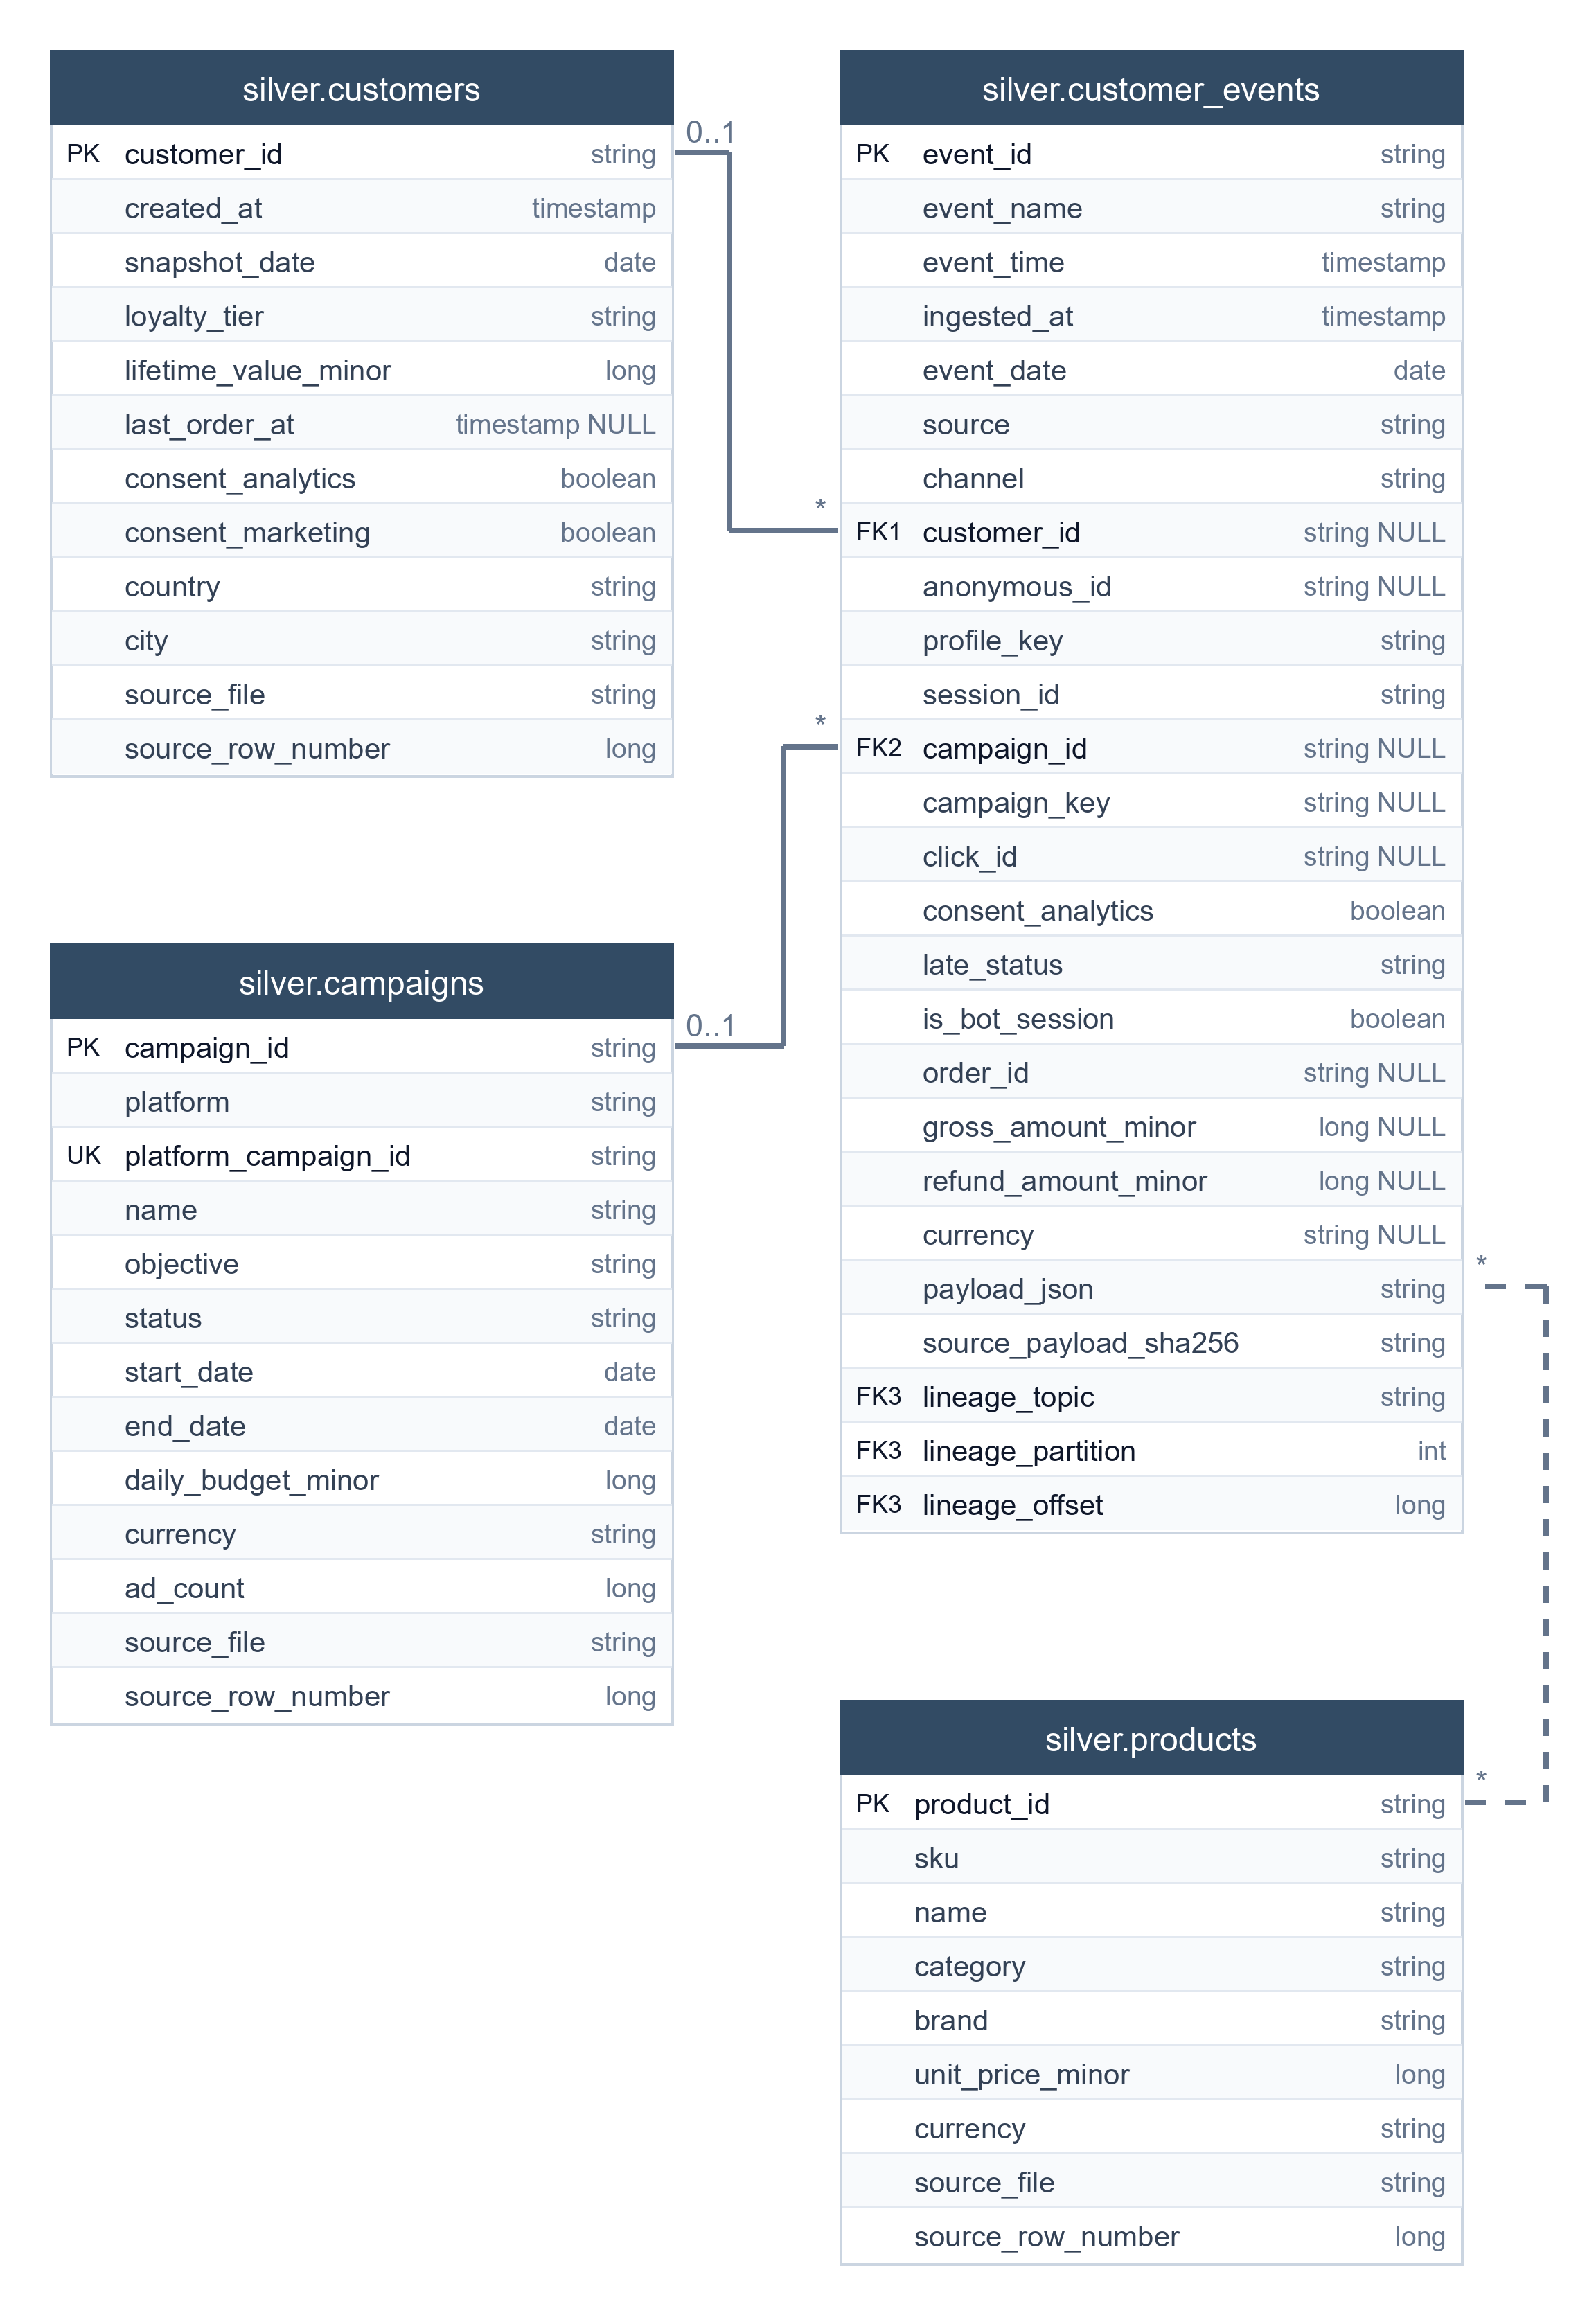
\includegraphics[width=\textwidth, height=0.86\textheight, keepaspectratio]{chapters/Pics/schema-silver-1.png}
    \caption{Lược đồ quan hệ tầng Silver (phần 1): sự kiện khách hàng và các bảng danh mục}
    \label{fig:schema-silver}
\end{figure}

\begin{figure}[!htbp]
    \centering
    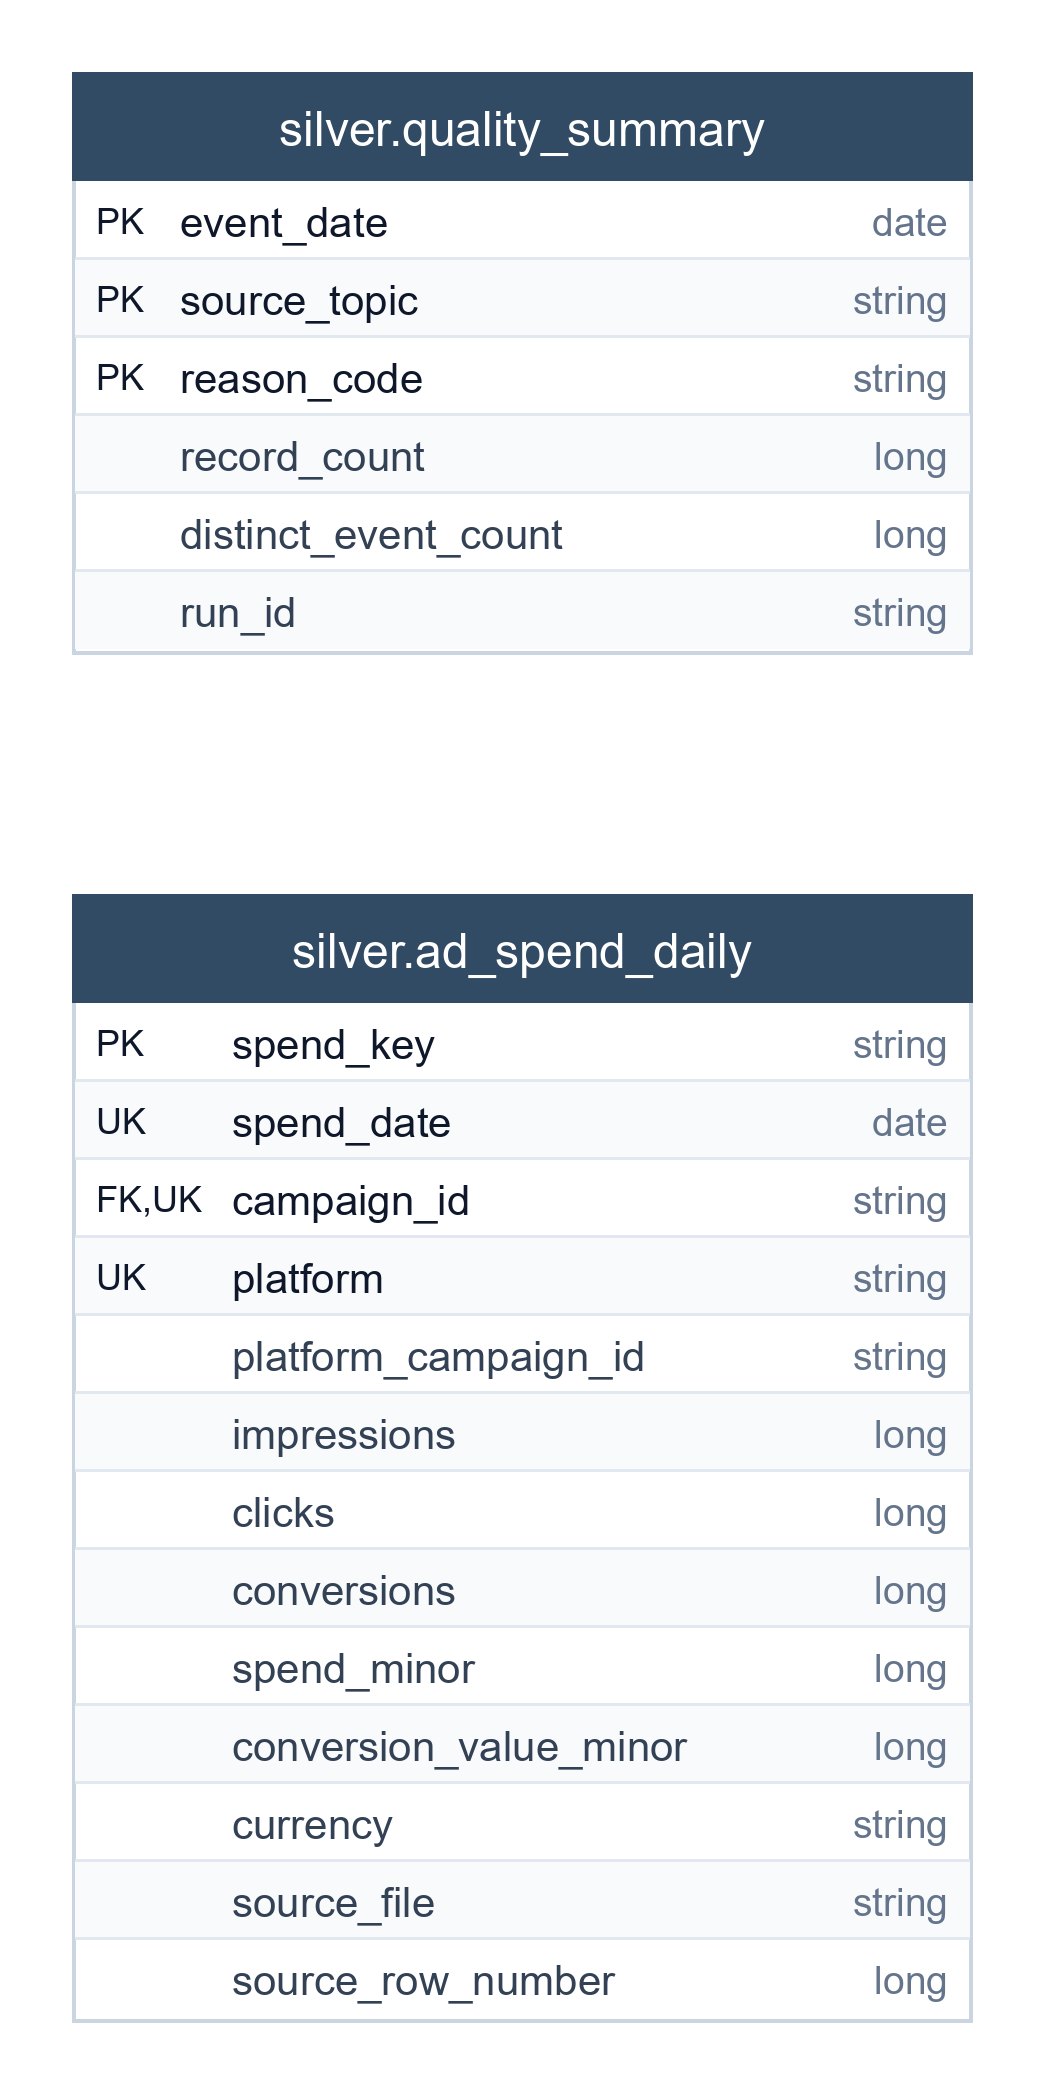
\includegraphics[width=0.42\textwidth]{chapters/Pics/schema-silver-2.png}
    \caption[Lược đồ quan hệ tầng Silver (phần 2): chi phí quảng cáo và thống kê chất lượng]{Lược đồ quan hệ tầng Silver (phần 2): chi phí quảng cáo và thống kê chất lượng. Khóa ngoại \texttt{campaign\_id} của \texttt{silver.ad\_spend\_daily} trỏ tới \texttt{silver.campaigns} ở Hình~\ref{fig:schema-silver}}
    \label{fig:schema-silver-2}
\end{figure}

\section{Lựa chọn lưu trữ và phương án thay thế}
\label{sec:c2-luu-tru-thay-the}

\subsection{Phân tách lưu trữ theo tải truy cập}
\label{sec:c2-phan-tach-luu-tru}

MarketPulse 360 không dùng một cơ sở dữ liệu cho mọi việc. Mỗi kiểu tải truy cập được giao cho hệ thống phù hợp nhất (Bảng~\ref{tab:components}): kho đối tượng giá rẻ cho dữ liệu gốc, định dạng bảng có giao dịch cho lịch sử, CSDL cột cho truy vấn phân tích độ trễ thấp và CSDL quan hệ cho dữ liệu vận hành cần ràng buộc chặt. Nhờ tách biệt, việc tính lại toàn bộ lịch sử trên Spark không ảnh hưởng đến người dùng đang đọc ClickHouse, và dữ liệu nghiệp vụ của ứng dụng (tài khoản, cấu hình, phân đoạn) không lẫn vào kho phân tích.

\begin{table}[!htbp]
\centering
\caption{Vai trò của các thành phần xử lý, lưu trữ và giám sát}
\label{tab:components}
\small
\renewcommand{\arraystretch}{1.2}
\begin{tabularx}{\textwidth}{>{\raggedright\arraybackslash}p{3.2cm} >{\raggedright\arraybackslash}p{2.3cm} >{\raggedright\arraybackslash}X}
\toprule
\textbf{Thành phần} & \textbf{Loại} & \textbf{Vai trò trong MarketPulse 360} \\
\midrule
Apache Kafka 4.3.1 & Xử lý (truyền tải) & Trục sự kiện chung, lưu nhật ký có thứ tự để phát lại \\
Apicurio Registry 3.3.3 & Hợp đồng dữ liệu & JSON Schema có phiên bản cho 10 topic \\
Apache Flink 2.2.1 & Xử lý luồng & Kiểm tra, khử trùng, gom phiên, chỉ số trực tiếp, exactly-once \\
Apache Spark 4.0.4 & Xử lý lô & Xây dựng Bronze, Silver, Gold trên Iceberg \\
Dagster 1.13 & Điều phối & Lập lịch và quản lý phụ thuộc giữa 13 tài sản dữ liệu \\
dbt Core 1.12 & Biến đổi, kiểm thử & Xây dựng 9 mô hình phục vụ và chạy kiểm thử trước công bố \\
\midrule
MinIO & Lưu trữ đối tượng & File nguồn gốc và file dữ liệu Iceberg \\
Apache Iceberg 1.12.0 & Định dạng bảng & Snapshot có giao dịch, phân vùng ẩn, truy vấn theo phiên bản \\
Project Nessie 0.109.0 & Catalog & Quản lý danh mục bảng Iceberg, lưu trên PostgreSQL riêng \\
ClickHouse 26.8 & CSDL cột (OLAP) & Phục vụ release đã kiểm chứng và số liệu trực tiếp \\
PostgreSQL 17.6 & CSDL quan hệ (OLTP) & Tài khoản, cấu hình, cảnh báo, phân đoạn, sổ cái công bố \\
\midrule
Prometheus 3.14 và Grafana 13.2 & Giám sát & Thu chỉ số năm giây một lần (độ trễ tiêu thụ Kafka, trạng thái và checkpoint của Flink, bộ nhớ ClickHouse, độ trễ và lỗi của API); 9 luật cảnh báo, 18 bảng biểu \\
\bottomrule
\end{tabularx}
\end{table}

\subsection{Tầng xử lý luồng: Flink và Kafka Streams}
\label{sec:c2-alt-streaming}

Kafka Streams là lựa chọn thay thế tự nhiên của Flink: nó là thư viện nhúng vào ứng dụng Java, không cần cụm riêng và cũng hỗ trợ exactly-once. Ưu điểm này đáng giá với các luồng nhỏ. Tuy nhiên, Flink cung cấp sẵn thời gian sự kiện với watermark, bộ hẹn giờ theo thời gian sự kiện để đóng phiên, trạng thái có TTL và cơ chế khôi phục từ checkpoint, đúng những gì đường ống luồng của MarketPulse 360 cần. Nhóm vì vậy chọn Flink làm động cơ chính và dùng Kafka Streams làm đối chứng trong một thực nghiệm có kiểm soát trên cùng khối lượng công việc (Mục~\ref{sec:c5-flink-vs-streams}).

\subsection{Tầng phục vụ: ClickHouse, PostgreSQL, BigQuery}
\label{sec:c2-alt-serving}

Với tầng phục vụ, phương án đối chứng là PostgreSQL, một CSDL lưu theo dòng, dùng chỉ mục B-tree. Nếu PostgreSQL đủ nhanh, hệ thống có thể bỏ bớt một thành phần. Thực nghiệm ở Mục~\ref{sec:c5-clickhouse-vs-postgres} so sánh hai hệ thống trên cùng một bảng dữ liệu mô phỏng có cấu trúc giống tầng Gold, ở các quy mô 1, 10 và 20 triệu dòng. Google BigQuery cùng BigLake là phương án đám mây có thể đọc trực tiếp bảng Iceberg; phương án này được cân nhắc nhưng chưa được đo đạc vì giới hạn tài nguyên đám mây của nhóm, và báo cáo không đưa ra kết luận nào về nó.


\newpage
\chapter{Công nghệ quản lý và xử lý dữ liệu}
\label{chap:cong-nghe}
% =============================================================================
% CHƯƠNG 3 — CÔNG NGHỆ QUẢN LÝ DỮ LIỆU, XỬ LÝ DỮ LIỆU VÀ QUY TRÌNH KIỂM CHỨNG
% Nội dung đối chiếu với repo marketpulse-360 @ dbe614b.
% =============================================================================

Chương này trình bày bốn cụm công nghệ cốt lõi của MarketPulse 360. Mỗi cụm được mô tả theo cùng một trình tự: công nghệ là gì và đóng vai trò gì, nó vận hành ra sao trong hệ thống, và những điểm hiện thực đáng chú ý. Cuối chương là năm ví dụ minh họa truy vết trực tiếp trên dữ liệu và mã nguồn.

\section{Apache Kafka và Apicurio Registry}
\label{sec:c3-kafka}

\subsection{Định nghĩa và vai trò}
\label{sec:c3-kafka-dinh-nghia}
Apache Kafka là nền tảng truyền dữ liệu phân tán dựa trên \emph{nhật ký chỉ ghi thêm} (append-only log)~\cite{kreps2011kafka, kafkadocs}. Mỗi topic được chia thành nhiều partition; bản ghi trong một partition có thứ tự và được định vị bằng offset, nên người tiêu thụ có thể đọc lại từ bất kỳ vị trí nào. Trong MarketPulse 360, Kafka 4.3.1 chạy ở chế độ KRaft (không cần ZooKeeper) và đóng vai trò \emph{trục sự kiện chung}: mọi sự kiện đều đi qua Kafka trước khi được nhánh luồng và nhánh lô tiêu thụ. Hai nhánh không độc lập hoàn toàn, vì nhánh lô dựng tầng Silver từ đầu ra của Flink (Mục~\ref{sec:c3-lakehouse-co-che}). Apicurio Registry 3.3.3~\cite{apicurio} lưu các hợp đồng dữ liệu (JSON Schema) có phiên bản cho từng topic.

\subsection{Cơ chế hoạt động}
\label{sec:c3-kafka-co-che}
Hệ thống dùng mười topic có phiên bản \texttt{v1}, chia thành bốn nhóm theo mức độ xử lý (Bảng~\ref{tab:kafka-topics}). Topic \texttt{raw} nhận dữ liệu nguồn từ công cụ phát lại; topic \texttt{clean} và \texttt{gold} do Flink ghi ra; hai topic \texttt{dlq} chứa bản ghi lỗi ở phía producer và phía Flink. Khóa phân vùng được chọn theo khóa nghiệp vụ: ưu tiên \texttt{customer\_id}, nếu không có thì dùng \texttt{session\_id}, \texttt{order\_id} hoặc \texttt{message\_id} tùy topic. Kafka chỉ giữ thứ tự trong một partition, nên cách chọn khóa này bảo đảm thứ tự cho các sự kiện cùng khóa trong cùng một topic: mọi sự kiện của một khách đã định danh nằm chung một partition, còn sự kiện của khách ẩn danh được nhóm theo phiên. Vì vậy, các phiên khác nhau của cùng một thiết bị ẩn danh có thể nằm ở các partition khác nhau, và Kafka không bảo đảm thứ tự giữa các topic.

\begin{table}[H]
\centering
\caption{Cấu hình các Kafka topic}
\label{tab:kafka-topics}
\footnotesize
\renewcommand{\arraystretch}{1.2}
\begin{tabularx}{\textwidth}{>{\raggedright\arraybackslash}p{6.3cm} >{\centering\arraybackslash}p{1.6cm} >{\raggedright\arraybackslash}p{2.6cm} >{\raggedright\arraybackslash}X}
\toprule
\textbf{Topic} & \textbf{Partition} & \textbf{Chính sách lưu} & \textbf{Khóa / bên ghi} \\
\midrule
\texttt{marketing.raw.web-events.v1} & 6 & delete, 7 ngày & khách hàng hoặc phiên; replay \\
\texttt{marketing.raw.order-events.v1} & 6 & delete, 7 ngày & khách hàng hoặc đơn hàng; replay \\
\texttt{marketing.raw.email-events.v1} & 6 & delete, 7 ngày & khách hàng hoặc email; replay \\
\texttt{marketing.dlq.validation.v1} & 6 & delete, 7 ngày & ca lỗi; replay \\
\texttt{marketing.clean.customer-events.v1} & 6 & delete, 7 ngày & \texttt{identity\_key}; Flink \\
\texttt{marketing.clean.sessions.v1} & 6 & compact, delete, 7 ngày & phiên; Flink \\
\texttt{marketing.gold.funnel-metrics.v1} & 3 & compact, delete, 30 ngày & \texttt{metric\_key}; Flink \\
\texttt{marketing.gold.revenue-metrics.v1} & 3 & compact, delete, 30 ngày & \texttt{metric\_key}; Flink \\
\texttt{marketing.gold.campaign-metrics.v1} & 3 & compact, delete, 30 ngày & \texttt{metric\_key}; Flink \\
\texttt{marketing.dlq.flink-validation.v1} & 6 & delete, 7 ngày & mã lỗi; Flink \\
\bottomrule
\end{tabularx}
\end{table}

Topic phiên và topic \texttt{gold} dùng chính sách \emph{compact}: Kafka chỉ giữ giá trị mới nhất của mỗi khóa, phù hợp với dữ liệu dạng ``trạng thái hiện tại'' như chỉ số của một chiến dịch trong ngày. Trước khi phát lại, mười hợp đồng JSON Schema được đăng ký lên Apicurio: hợp đồng chưa có thì tạo mới, hợp đồng đã có chỉ được thêm phiên bản khi nội dung thật sự thay đổi.

\subsection{Điểm nổi bật trong MarketPulse 360}
\label{sec:c3-kafka-hien-thuc}
\begin{itemize}
    \item \textbf{Gửi lại không tạo bản sao.} Producer bật \texttt{enable.idempotence} và \texttt{acks=all}; nếu một lần gửi bị lỗi và producer tự gửi lại trong cùng phiên, Kafka không ghi thêm bản sao vào partition. Bảo đảm này chỉ áp dụng cho việc gửi lại; bản ghi trùng có sẵn trong dữ liệu nguồn vẫn đi vào Kafka và được Flink, Silver khử trùng sau đó.
    \item \textbf{Phát lại an toàn.} Con trỏ phát lại lưu vị trí đã gửi và gắn với mã băm của manifest dữ liệu. Nếu xác nhận gửi không rõ ràng hoặc thế giới dữ liệu đã thay đổi, công cụ dừng lại thay vì đoán.
    \item \textbf{Tách biệt hợp đồng và dữ liệu.} Hợp đồng JSON Schema được quản lý tập trung, giúp bản ghi lỗi bị chặn ngay ở cửa vào và được chuyển sang DLQ thay vì làm hỏng các bảng phía sau.
\end{itemize}

\section{Apache Flink}
\label{sec:c3-flink}

\subsection{Định nghĩa và vai trò}
\label{sec:c3-flink-dinh-nghia}
Apache Flink là động cơ xử lý luồng phân tán có trạng thái~\cite{carbone2015flink, flinkdocs}. Flink xử lý từng sự kiện ngay khi đến, cho phép lưu trạng thái theo khóa và khôi phục trạng thái đó sau sự cố nhờ cơ chế checkpoint nhất quán~\cite{carbone2017state}. Flink hỗ trợ \emph{thời gian sự kiện} với watermark (ý tưởng xuất phát từ mô hình Dataflow~\cite{akidau2015dataflow}) nên xử lý đúng cả khi sự kiện đến không theo thứ tự. Trong MarketPulse 360, Flink 2.2.1 là bộ não của nhánh luồng: làm sạch sự kiện và tính chỉ số chiến dịch trong vài giây.

\subsection{Cơ chế hoạt động}
\label{sec:c3-flink-co-che}
Job \texttt{marketpulse-stream-v1} gồm một chuỗi toán tử có định danh ổn định (Hình~\ref{fig:flink}):

\begin{enumerate}
    \item \textbf{Đọc và gán thời gian sự kiện.} Nguồn Kafka đọc ba topic \texttt{raw}; watermark cho phép sự kiện lệch tối đa 5 phút và đánh dấu partition nhàn rỗi sau 1 phút để watermark không bị kẹt.
    \item \textbf{Kiểm tra hợp đồng.} Bản ghi không đúng hợp đồng được tách sang side output và ghi vào \texttt{marketing.dlq.flink-validation.v1} kèm mã lỗi, không làm dừng job.
    \item \textbf{Khử trùng lặp.} Luồng được phân theo \texttt{event\_id}; trạng thái \texttt{ValueState} ghi nhớ sự kiện đã thấy trong 7 ngày (TTL \num{604800000} ms) và loại mọi bản sao.
    \item \textbf{Phân loại sự kiện trễ.} Sự kiện đến sau watermark nhưng trong ngưỡng sửa 10 phút vẫn được cập nhật vào chỉ số; sự kiện trễ hơn được ghi nhận để kiểm toán.
    \item \textbf{Gom phiên.} Theo \texttt{session\_id}, bộ hẹn giờ theo thời gian sự kiện đóng phiên sau 30 phút không hoạt động.
    \item \textbf{Chỉ số chiến dịch.} Theo \texttt{metric\_key} (chiến dịch $\times$ ngày), trạng thái tích lũy số phiên ở từng bước phễu, số đơn, doanh thu gộp, hoàn tiền và doanh thu ròng.
    \item \textbf{Ghi exactly-once.} Một sink Kafka duy nhất định tuyến bản ghi tới đúng topic và ghi theo giao thức two-phase commit với tiền tố giao dịch \texttt{marketpulse-flink-v1-}. Checkpoint chạy mỗi 5 giây ở chế độ exactly-once.
\end{enumerate}

\begin{figure}[!htbp]
    \centering
    \resizebox{\textwidth}{!}{\input{chapters/Figs/fig-flink-topology}}
    \caption{Topology chuỗi toán tử xử lý luồng có trạng thái trên Apache Flink}
    \label{fig:flink}
\end{figure}

\subsection{Điểm nổi bật trong MarketPulse 360}
\label{sec:c3-flink-hien-thuc}
Điểm quan trọng nhất là \emph{tính nhất quán khi có sự cố}. Offset nguồn, trạng thái khử trùng, trạng thái phiên và chỉ số chiến dịch được lưu trong cùng một checkpoint, còn kết quả chỉ hiển thị cho người đọc sau khi giao dịch Kafka được commit. Vì vậy, khi một TaskManager bị khởi động lại, job tiếp tục từ checkpoint gần nhất mà không đếm thiếu hay đếm trùng (Ví dụ~1, Mục~\ref{sec:c3-vi-du-1}). Mọi toán tử đều có \texttt{uid} cố định, nên có thể nâng cấp job mà vẫn khôi phục được trạng thái cũ. Bộ gửi job cũng được thiết kế lũy đẳng: nó nhận ra job đang chạy ở mọi trạng thái chưa kết thúc và không tạo job thứ hai.

\section{Lakehouse: MinIO, Iceberg, Nessie và Spark}
\label{sec:c3-lakehouse}

\subsection{Định nghĩa và vai trò}
\label{sec:c3-lakehouse-dinh-nghia}
Kiến trúc \emph{lakehouse} kết hợp chi phí thấp của hồ dữ liệu với tính giao dịch của kho dữ liệu~\cite{armbrust2021lakehouse}. MarketPulse 360 hiện thực kiến trúc này bằng bốn thành phần: MinIO là kho đối tượng tương thích S3~\cite{minio}; Apache Iceberg 1.12.0 là định dạng bảng mở với snapshot có giao dịch và phân vùng ẩn~\cite{icebergspec}; Project Nessie 0.109.0 là catalog quản lý danh mục bảng~\cite{nessie}; Apache Spark 4.0.4 là động cơ tính toán lô~\cite{zaharia2012rdd, sparkdocs}.

\subsection{Cơ chế hoạt động}
\label{sec:c3-lakehouse-co-che}
\textbf{Tầng Bronze.} Bronze lưu năm topic: ba topic \texttt{raw}, topic \texttt{clean.customer-events} và topic \texttt{dlq.flink-validation} của Flink; các topic \texttt{gold} không được lưu vì có thể tính lại từ Silver. Spark đọc Kafka ở chế độ \texttt{read\_committed} theo một khoảng offset xác định, nên chỉ thấy bản ghi của giao dịch đã commit. Mỗi lần chạy đọc tiếp từ offset lớn nhất đã có trong Bronze đến offset mới nhất trên broker. Retention 7 ngày của Kafka vì vậy cũng là ràng buộc của nhánh lô: nếu nhánh lô ngừng chạy lâu hơn 7 ngày, các offset cần đọc có thể đã bị Kafka xóa, và lần chạy dừng với lỗi \texttt{Kafka retention gap} (cấu hình \texttt{failOnDataLoss=true}) thay vì âm thầm bỏ sót dữ liệu; khi đó phải phát lại dữ liệu từ nguồn. Bản ghi đã vào Bronze thì được lưu lâu dài trên Iceberg. Việc ghi dùng \texttt{MERGE} theo khóa \texttt{ingest\_id}; nếu cùng một khóa xuất hiện với nội dung khác, quá trình dừng với lỗi va chạm khóa bất biến. File nguồn được kiểm tra kích thước và mã băm so với manifest trước khi lưu.

\textbf{Tầng Silver.} Spark giải mã các sự kiện \texttt{clean}, gom các bản sao theo \texttt{event\_id} và chọn bản thắng theo thứ tự xác định. Phiên bản 1 của hợp đồng \texttt{clean} không mang \texttt{click\_id}, nên Silver nối ngược về bản ghi \texttt{raw} qua bộ ba lineage để khôi phục trường này, đồng thời kiểm tra \texttt{event\_id} hai phía phải trùng nhau. Sự kiện không có đồng thuận phân tích bị loại với mã \texttt{CONSENT\_DENIED}, sự kiện bị Flink đánh dấu trễ quá ngưỡng bị loại với mã \texttt{LATE\_INELIGIBLE}, phiên bot web/app bị loại với mã \texttt{BOT\_EXCLUDED}; mọi quyết định đều được đếm trong \texttt{silver.quality\_summary}.

\textbf{Phụ thuộc giữa nhánh lô và Flink.} Vì Silver dựng \texttt{silver.customer\_events} từ topic \texttt{clean}, nhánh lô kế thừa các quyết định của Flink: kết quả kiểm tra hợp đồng, cách phân loại sự kiện trễ và giá trị các trường đã chuẩn hóa. Silver có một lớp đối soát với dữ liệu gốc: mọi offset của topic \texttt{raw} phải có đúng một kết cục (nằm trong \texttt{clean}, nằm trong DLQ, hoặc là bản sao của một sự kiện đã nhận), thiếu một offset là cả lô thất bại. Tuy nhiên, Silver không tự tính lại giá trị của từng trường từ dữ liệu \texttt{raw}. Nếu Flink có lỗi logic, chẳng hạn chuẩn hóa sai số tiền, lỗi đó sẽ đi vào số liệu đã kiểm chứng. Trên dữ liệu mô phỏng, lớp kiểm tra độc lập với Flink là oracle story-demo: nó tính lại các chỉ số trực tiếp từ file nguồn của bộ sinh, không đi qua đường ống, và phát hiện được loại lỗi này (Mục~\ref{sec:c5-oracle}). Với dữ liệu thật, cần bổ sung một phép đối soát giá trị độc lập giữa \texttt{raw} và \texttt{clean} (Mục~\ref{sec:c6-huong-phat-trien}).

\textbf{Tầng Gold.} Spark xây dựng sáu bảng phân tích. Phép phân bổ doanh thu tìm các click trả phí của cùng hồ sơ trong cửa sổ 30 ngày trước đơn hàng, rồi chia tiền theo ba mô hình First-Touch, Last-Touch và Linear; đơn hàng không có điểm chạm nào được gán cho \texttt{\_\_unattributed\_\_} để tổng tiền luôn bảo toàn.

\subsection{Điểm nổi bật trong MarketPulse 360}
\label{sec:c3-lakehouse-hien-thuc}
\begin{itemize}
    \item \textbf{Tái lập theo snapshot.} Mỗi lần chuẩn bị dữ liệu sinh một \emph{phiếu chuẩn bị} (preparation receipt) ghi lại mã snapshot của từng bảng Bronze, Silver và Gold. Nhờ truy vấn theo phiên bản của Iceberg (\texttt{VERSION AS OF}), mọi tính toán sau đó đều đọc đúng trạng thái đã ghim, kể cả khi bảng nguồn đã có dữ liệu mới.
    \item \textbf{Không gian tên cô lập.} Mỗi lần chuẩn bị ghi Silver và Gold vào một namespace riêng \texttt{mp\_batch\_<identity>\_<attempt>}, nên một lần chạy lỗi không bao giờ làm hỏng kết quả trước đó.
    \item \textbf{Tiền là số nguyên.} Mọi số tiền được lưu bằng đơn vị nhỏ nhất (VND) kiểu \texttt{long}; phép chia luôn là phép chia nguyên có phân bổ phần dư (Ví dụ~3).
    \item \textbf{Phân vùng phù hợp truy vấn.} Bảng sự kiện phân vùng theo tháng, bảng Kafka phân vùng theo ngày, giúp truy vấn lịch sử và tính lại chỉ quét đúng phần dữ liệu liên quan.
\end{itemize}

\section{Dagster, dbt và ClickHouse}
\label{sec:c3-dagster-dbt-clickhouse}

\subsection{Định nghĩa và vai trò}
\label{sec:c3-dagster-dinh-nghia}
Dagster 1.13 là công cụ điều phối theo mô hình \emph{tài sản dữ liệu định nghĩa bằng phần mềm} (Software-Defined Assets): thay vì mô tả các tác vụ, người phát triển mô tả các bảng cần có và phụ thuộc giữa chúng~\cite{dagsterdocs}. dbt Core 1.12 biến đổi dữ liệu bằng SQL có quản lý phiên bản và chạy kiểm thử dữ liệu như kiểm thử phần mềm~\cite{dbtdocs}. ClickHouse 26.8 là CSDL lưu theo cột tối ưu cho truy vấn phân tích, dùng họ động cơ bảng MergeTree~\cite{clickhousedocs}.

\subsection{Cơ chế hoạt động}
\label{sec:c3-dagster-co-che}
Đồ thị gồm 13 định nghĩa tài sản chia thành ba giai đoạn (Hình~\ref{fig:dagster}). Lịch \texttt{daily\_marketing\_refresh} chạy lúc 02:00 hằng ngày cho ngày hôm trước thông qua job \texttt{marketing\_refresh\_job}. Job \texttt{historical\_rebuild\_job} chạy lại toàn bộ đồ thị trừ bước công bố, dùng để tính lại lịch sử một cách cô lập; job \texttt{source\_history\_job} nạp lần đầu dữ liệu nguồn cho các ngày quá khứ.

\begin{figure}[H]
    \centering
    \resizebox{\textwidth}{!}{\input{chapters/Figs/fig-dagster}}
    \caption{Đồ thị phụ thuộc các tài sản dữ liệu trên Dagster}
    \label{fig:dagster}
\end{figure}

Sau khi Gold được xây xong, snapshot được xuất thành file JSON kèm manifest có checksum, rồi nạp vào một CSDL ClickHouse \emph{ứng viên} mới tinh \texttt{mp\_release\_<identity>\_<attempt>}. Tám bảng \texttt{raw\_*} trong CSDL này là nguồn của dbt; dbt dựng chín mô hình và chạy 31 bài kiểm thử (Bảng~\ref{tab:dbt}). Chỉ khi mọi bước của quy trình trong Hình~\ref{fig:certification} thành công, bản phát hành mới được công bố.

\begin{figure}[H]
    \centering
    \resizebox{\textwidth}{!}{% Hình 3.3 — Kiểm chứng bản phát hành cô lập và công bố nguyên tử
\begin{tikzpicture}[node distance=5mm, s/.style={mpbox=37mm, minimum height=19mm}]
  % Hàng 1: chuẩn bị và dựng ứng viên
  \node[s] (p1) {\textbf{1. Phiếu chuẩn bị}\\ ghim snapshot Bronze\\ \texttt{identity} = SHA-256};
  \node[s, right=of p1] (p2) {\textbf{2. Xuất snapshot}\\ file JSON + manifest\\ có checksum, lưu MinIO};
  \node[s, right=of p2] (p3) {\textbf{3. Nạp ứng viên}\\ CSDL \texttt{mp\_release\_*}\\ 8 bảng \texttt{raw\_*}};
  \node[s, right=of p3] (p4) {\textbf{4. dbt build}\\ 9 mô hình\\ 31 bài kiểm thử};
  % Hàng 2: đối soát và công bố (đi ngược từ phải sang trái)
  \node[s, below=8mm of p4] (p5) {\textbf{5. Đối soát checksum}\\ checksum từng bảng\\ oracle CTR/CPC\\ \texttt{proof\_digest}};
  \node[s, left=of p5] (p6) {\textbf{6. Ghi sổ cái}\\ \texttt{certified\_bundles}\\ \texttt{publications}\\ (PostgreSQL)};
  \node[s, left=of p6] (p7) {\textbf{7. Công bố}\\ \texttt{publication\_journal}\\ (ClickHouse)};
  \node[mphead=37mm, minimum height=19mm, left=of p7] (p8) {Ứng dụng đọc\\ \texttt{max(generation)}};
  % Nhánh thất bại
  \node[mpbox=60mm, below=8mm of p6, xshift=-21mm, draw=mpline, fill=mpzone] (fail)
    {\textbf{Bất kỳ bước nào thất bại}\\ ứng viên bị loại bỏ, release đang phục vụ giữ nguyên};

  \draw[mparrow] (p1) -- (p2);
  \draw[mparrow] (p2) -- (p3);
  \draw[mparrow] (p3) -- (p4);
  \draw[mparrow] (p4) -- (p5);
  \draw[mparrow] (p5) -- (p6);
  \draw[mparrow] (p6) -- (p7);
  \draw[mparrow] (p7) -- (p8);
  \draw[mpdash] (p5.south) |- (fail.east);
\end{tikzpicture}
}
    \caption{Quy trình kiểm chứng bản phát hành cô lập và công bố nguyên tử}
    \label{fig:certification}
\end{figure}

\subsection{Tầng Gold và các mô hình dbt}
\label{sec:c3-gold-schema}
Hình~\ref{fig:schema-gold} và Hình~\ref{fig:schema-gold-2} trình bày chín mô hình trong CSDL release, với kiểu dữ liệu ClickHouse. Sáu mô hình là bản sao chính xác của các bảng Iceberg \texttt{gold.*}; \texttt{campaigns} và \texttt{customers} là hai bảng chiều xuất từ Silver; \texttt{campaign\_dashboard} là mart làm giàu từ \texttt{campaign\_performance\_daily} (32 cột) và \texttt{campaigns}, bổ sung tên, trạng thái chiến dịch, CTR và CPC. Khóa ngoại tới \texttt{campaigns} được kiểm thử bởi \texttt{campaign\_relationships}, ngoại trừ giá trị đặc biệt \texttt{\_\_unattributed\_\_}; khóa ngoại tới \texttt{customers} được kiểm thử bởi \texttt{customer\_relationships}. Bảng \texttt{cohort\_retention} được tổng hợp từ \texttt{customer\_360} và hoạt động theo tháng nên được biểu diễn bằng quan hệ dẫn xuất.

\begin{figure}[!htbp]
    \centering
    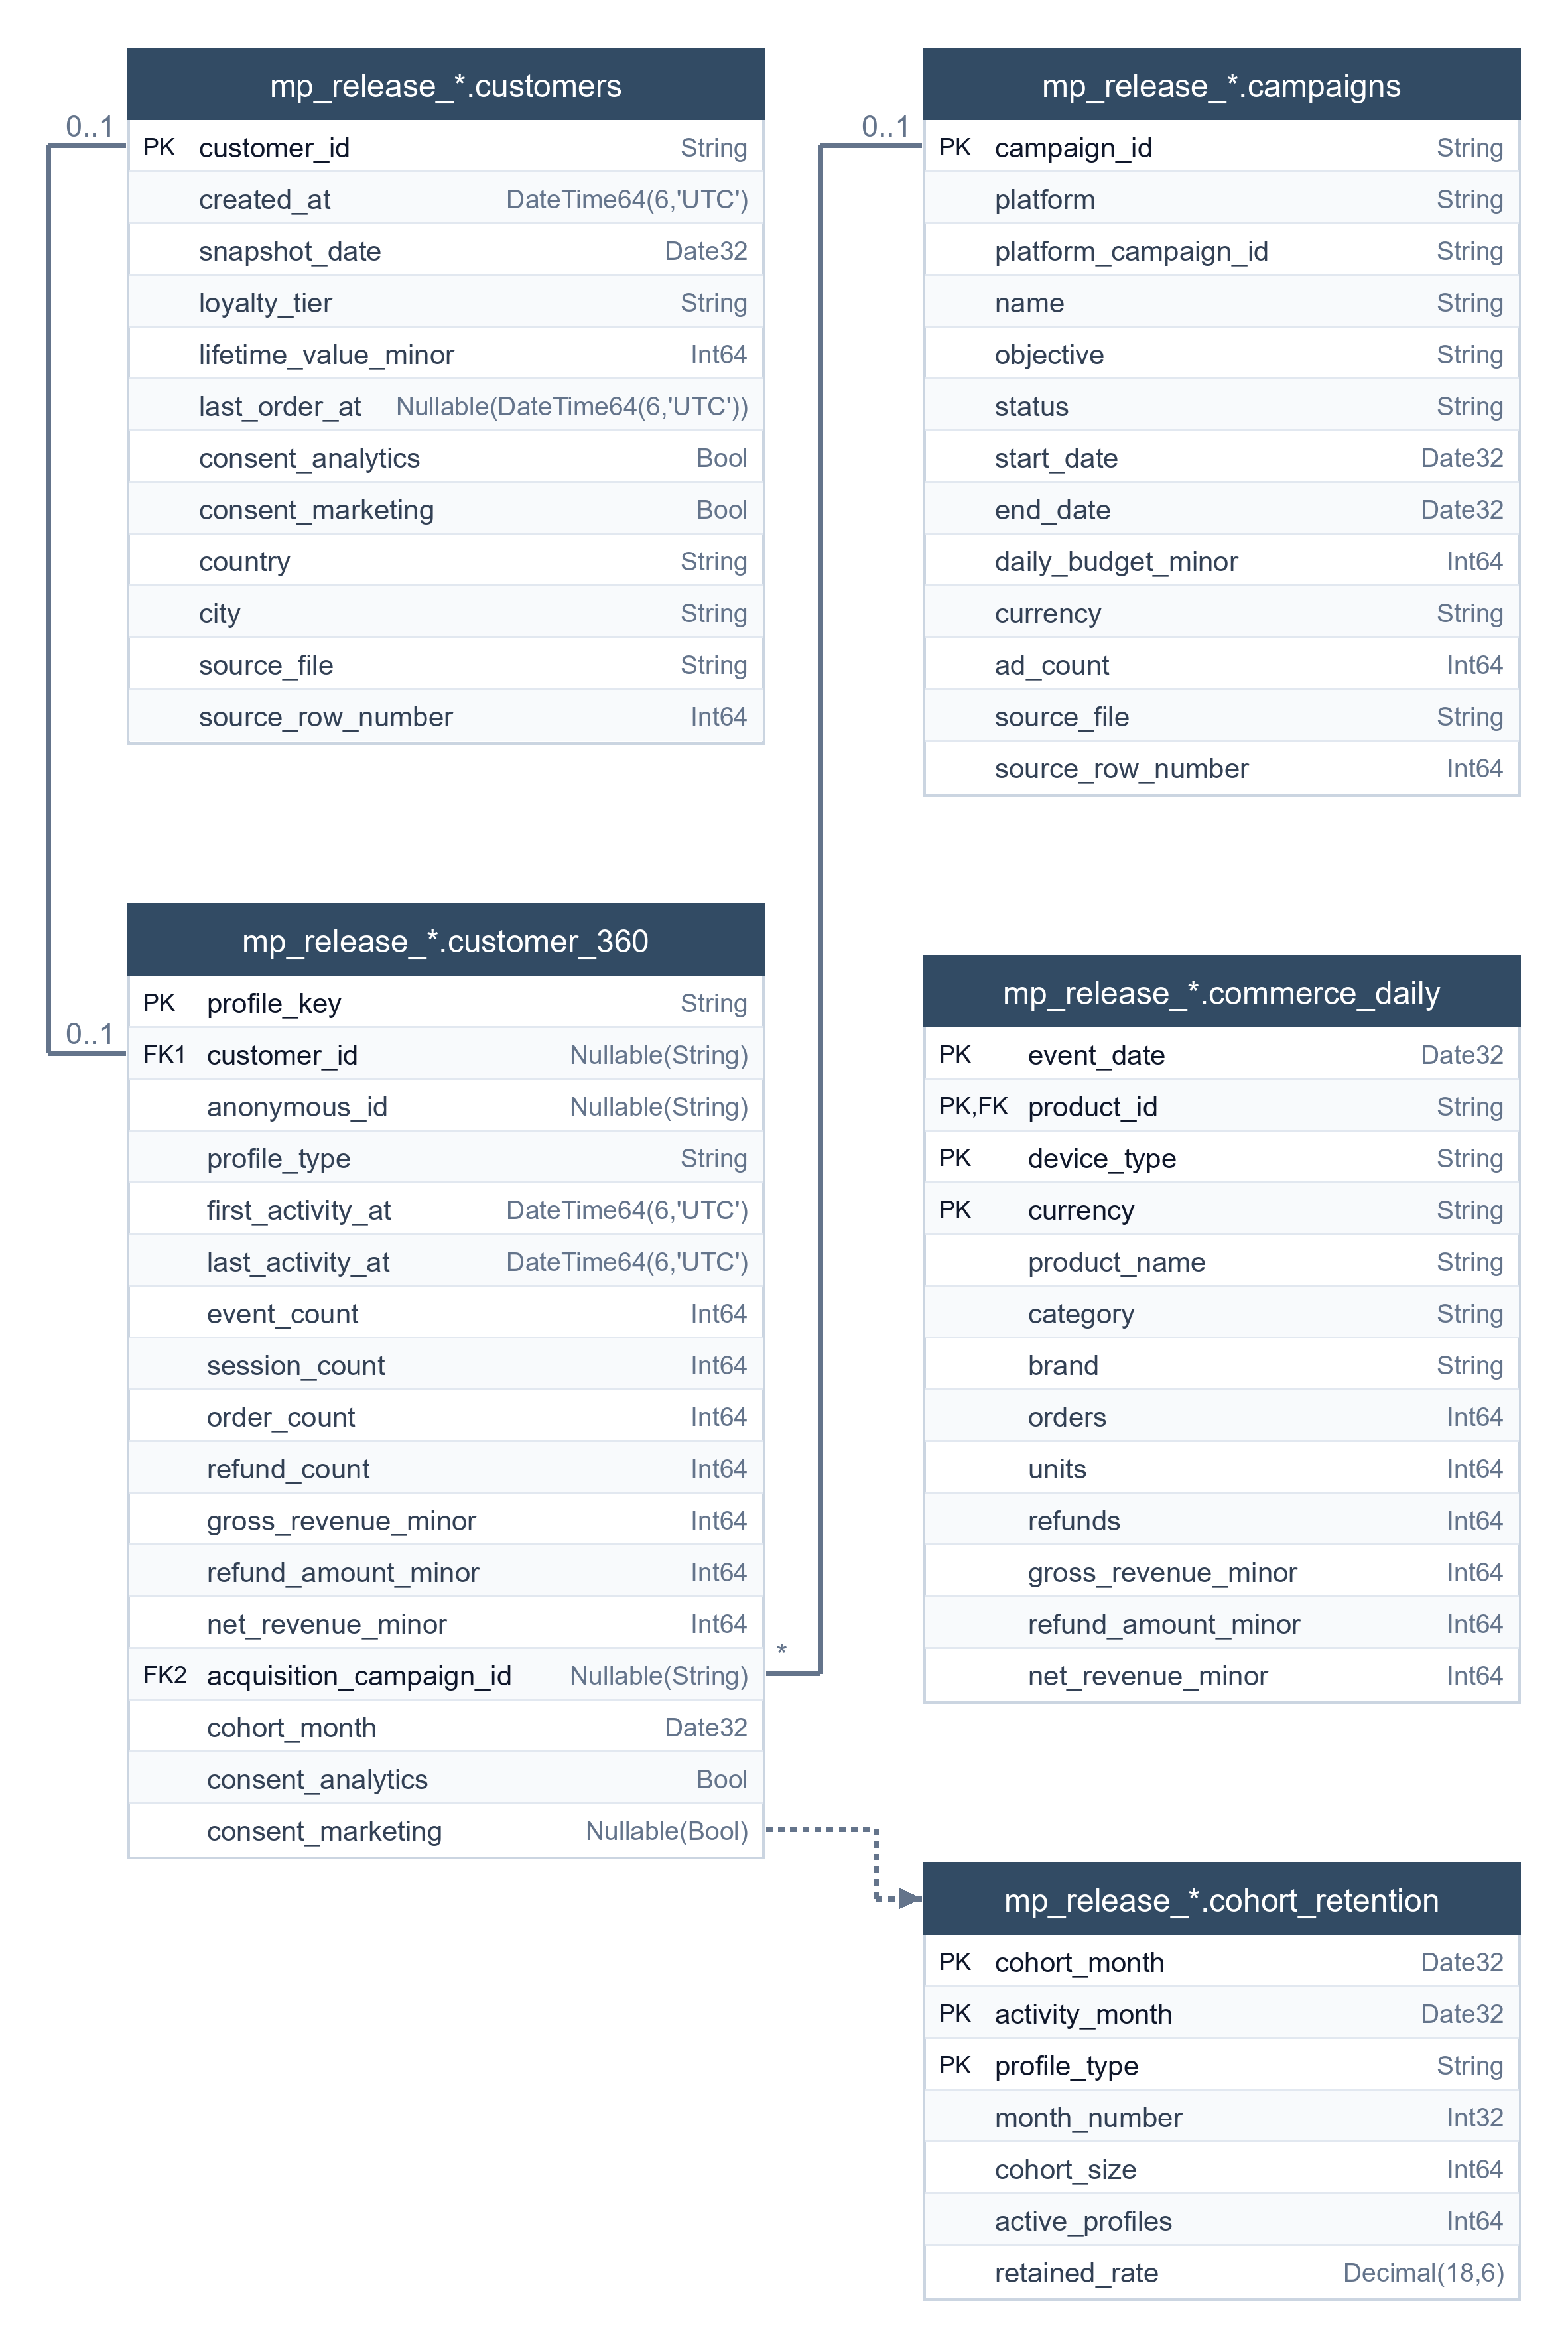
\includegraphics[width=\textwidth, height=0.86\textheight, keepaspectratio]{chapters/Pics/schema-gold-1.png}
    \caption{Lược đồ quan hệ các mô hình dbt phục vụ trên ClickHouse (phần 1): bảng chiều, Customer 360, thương mại và cohort}
    \label{fig:schema-gold}
\end{figure}

\begin{figure}[!htbp]
    \centering
    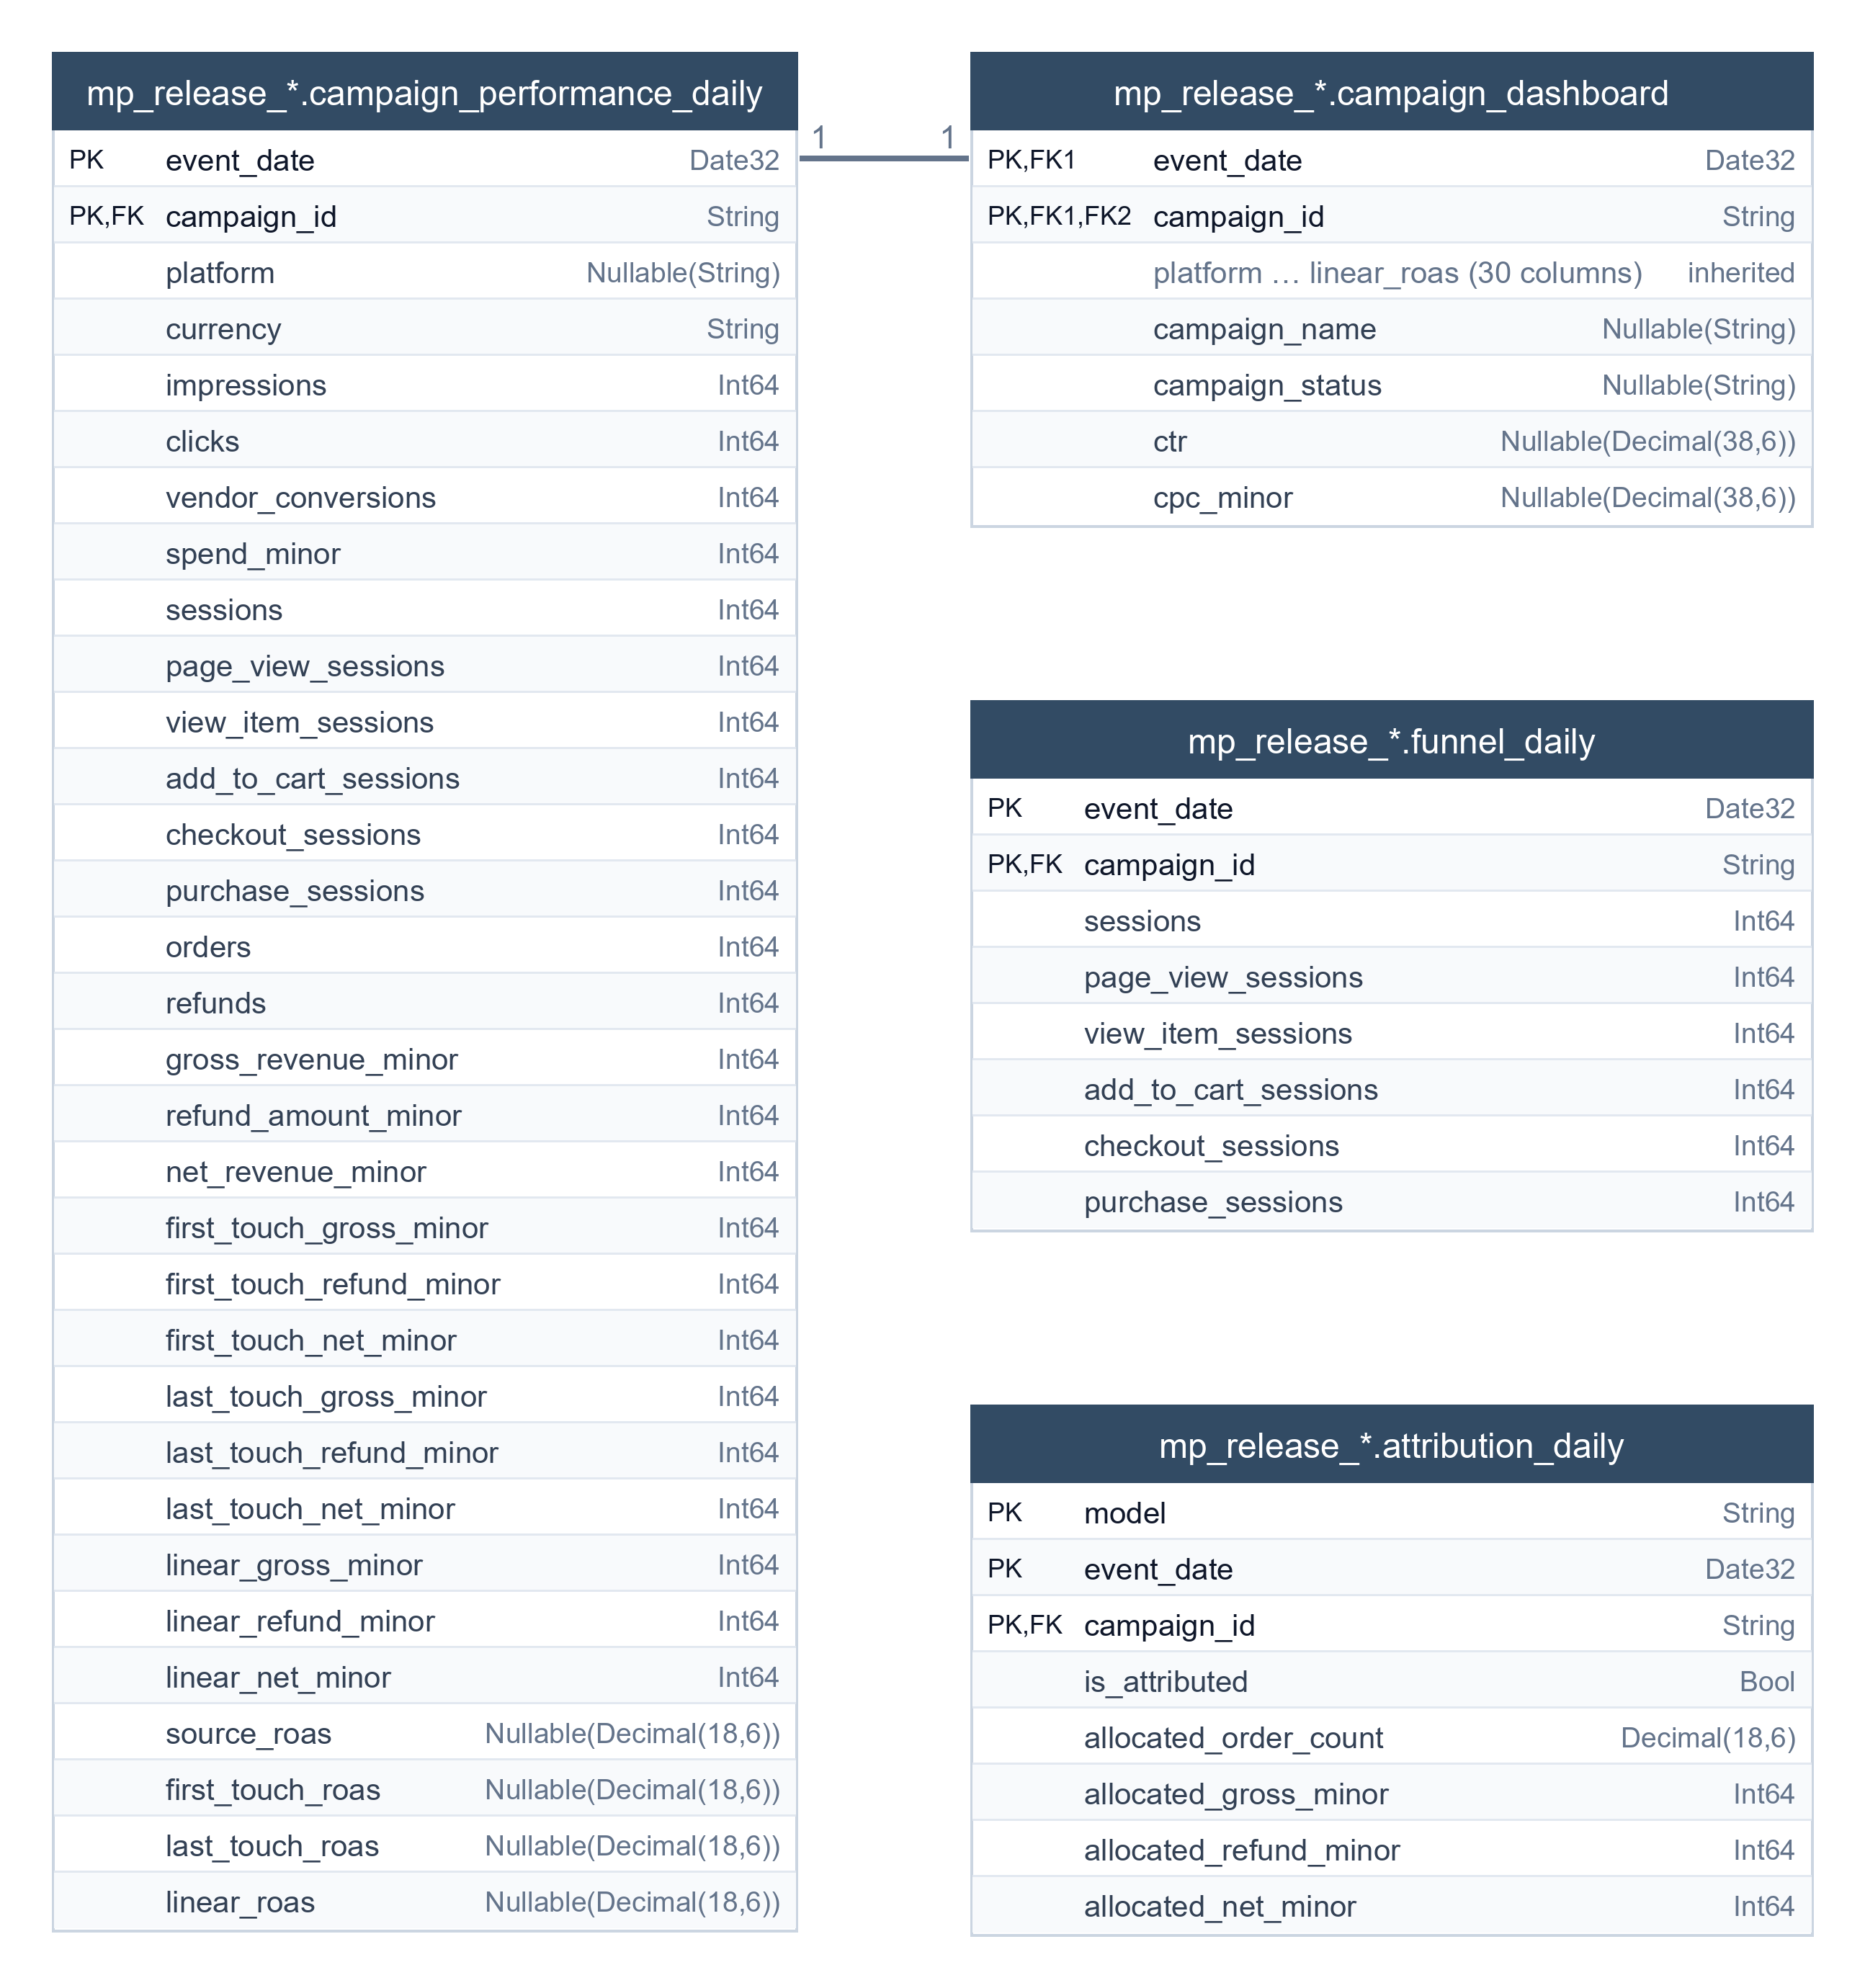
\includegraphics[width=\textwidth, height=0.86\textheight, keepaspectratio]{chapters/Pics/schema-gold-2.png}
    \caption[Lược đồ quan hệ các mô hình dbt phục vụ trên ClickHouse (phần 2): hiệu quả chiến dịch, phễu và phân bổ]{Lược đồ quan hệ các mô hình dbt phục vụ trên ClickHouse (phần 2): hiệu quả chiến dịch, phễu và phân bổ. Cột \texttt{campaign\_id} của bốn bảng là khóa ngoại tới \texttt{campaigns} ở Hình~\ref{fig:schema-gold}}
    \label{fig:schema-gold-2}
\end{figure}

\begin{table}[!htbp]
\centering
\caption{Các mô hình dbt và bài kiểm thử chất lượng dữ liệu tự động}
\label{tab:dbt}
\footnotesize
\renewcommand{\arraystretch}{1.2}
\begin{tabularx}{\textwidth}{>{\raggedright\arraybackslash}p{5.0cm} >{\raggedright\arraybackslash}p{5.7cm} >{\raggedright\arraybackslash}X}
\toprule
\textbf{Mô hình (ORDER BY)} & \textbf{Nguồn} & \textbf{Kiểm thử tổng quát} \\
\midrule
\texttt{campaign\_performance\_daily} & \texttt{raw\_campaign\_performance\_daily} & khóa duy nhất, cột bắt buộc \\
\texttt{funnel\_daily} & \texttt{raw\_funnel\_daily} & khóa duy nhất, cột bắt buộc, not null \\
\texttt{attribution\_daily} & \texttt{raw\_attribution\_daily} & khóa duy nhất, cột bắt buộc, giá trị hợp lệ \\
\texttt{customer\_360} & \texttt{raw\_customer\_360} & khóa duy nhất, cột bắt buộc, giá trị hợp lệ \\
\texttt{cohort\_retention} & \texttt{raw\_cohort\_retention} & khóa duy nhất, cột bắt buộc \\
\texttt{commerce\_daily} & \texttt{raw\_commerce\_daily} & khóa duy nhất, cột bắt buộc \\
\texttt{campaigns} & \texttt{raw\_campaigns} & khóa duy nhất, cột bắt buộc, not null \\
\texttt{customers} & \texttt{raw\_customers} & khóa duy nhất, cột bắt buộc, not null \\
\texttt{campaign\_dashboard} & \texttt{campaign\_performance\_daily} $\bowtie$ \texttt{campaigns} & khóa duy nhất \\
\midrule
\multicolumn{3}{>{\raggedright\arraybackslash}p{15.2cm}}{\textbf{Kiểm thử nghiệp vụ (9):} \texttt{financial\_equations} (gộp $-$ hoàn = ròng ở mọi bảng), \texttt{attribution\_conservation} (tổng phân bổ của mỗi mô hình bằng doanh thu Customer 360), \texttt{commerce\_conservation}, \texttt{campaign\_relationships}, \texttt{customer\_relationships}, \texttt{cohort\_invariants}, \texttt{funnel\_invariants}, \texttt{consent\_eligibility}, \texttt{accepted\_domains}.} \\
\midrule
\multicolumn{3}{l}{\textbf{Tổng cộng:} 22 kiểm thử tổng quát + 9 kiểm thử nghiệp vụ = 31 kiểm thử.} \\
\bottomrule
\end{tabularx}
\end{table}

\subsection{Điểm nổi bật trong MarketPulse 360}
\label{sec:c3-dagster-hien-thuc}
\begin{itemize}
    \item \textbf{Kiểm chứng trên dữ liệu thật của release.} Ngoài 31 bài kiểm thử dbt, bước đối soát checksum (bước 5 trong Hình~\ref{fig:certification}) tính checksum cho toàn bộ dòng của từng bảng và so với checksum lúc xuất, tính lại CTR, CPC bằng một oracle độc lập, rồi gộp mọi bằng chứng thành \texttt{proof\_digest}.
    \item \textbf{Công bố nguyên tử và đơn điệu.} Sổ cái PostgreSQL \texttt{marketpulse\_ops} giữ khóa tư vấn (advisory lock) khi đặt chỗ công bố và từ chối bản phát hành của một ngày logic cũ hơn bản đã công bố. Bản ghi được nối vào \texttt{publication\_journal} trên ClickHouse rồi mới được xác nhận; ứng dụng luôn đọc bản có \texttt{generation} lớn nhất. Một tiến trình công bố chậm vì thế không thể ``kéo lùi'' người đọc về bản cũ.
    \item \textbf{Không tái sử dụng ứng viên dở dang.} Mỗi lần nạp tạo một CSDL mới theo số lần thử; một CSDL nạp dở không bao giờ được dùng lại.
\end{itemize}

\section{Ví dụ minh họa}
\label{sec:c3-vi-du}

Năm ví dụ dưới đây được chọn để mỗi ví dụ minh họa một rủi ro điển hình của dữ liệu marketing và cách đường ống xử lý nó. Các con số đều lấy từ bằng chứng chạy thật trong kho mã~\cite{mp360repo}.

\subsection{Ví dụ 1: Khử trùng lặp và phục hồi trên Flink}
\label{sec:c3-vi-du-1}
Kịch bản kiểm thử phục hồi khởi động lại TaskManager của Flink \emph{trong khi} producer vẫn đang gửi dữ liệu, kèm hai bản sao trùng \texttt{event\_id} được chèn có chủ đích. Trong quá trình phục hồi, đầu vào Kafka thô tăng từ 83 lên 219 bản ghi. Sau khi job khôi phục từ checkpoint, đầu ra giữ đúng 217 mã sự kiện duy nhất và 73 khóa phiên, hai bản sao bị loại, và doanh thu ròng đối soát khớp \num{24751000}~VND. Kết quả cho thấy trạng thái khử trùng được khôi phục cùng offset nguồn: bản ghi đã xử lý trước sự cố không bị tính lại, bản ghi đến trong lúc sự cố không bị mất.

\subsection{Ví dụ 2: Khôi phục mã click tại tầng Silver}
\label{sec:c3-vi-du-2}
Một phiên mua hàng bắt đầu từ click quảng cáo trả phí có \texttt{click\_id} trong bản ghi \texttt{raw}, nhưng bản ghi \texttt{clean} phiên bản 1 không mang trường này. Silver dùng bộ ba \texttt{(lineage\_topic, lineage\_partition, lineage\_offset)} để tìm đúng bản ghi \texttt{raw} trong \texttt{bronze.kafka\_records}, đọc payload, kiểm tra \texttt{event\_id} trùng khớp rồi mới khôi phục \texttt{click\_id}; nhờ đó đơn hàng được phân bổ về đúng chiến dịch.

Cùng lúc, Silver áp dụng quản trị. Trên tập fixture, doanh thu ròng của luồng chưa quản trị là \num{24751000}~VND, còn doanh thu đã quản trị được công bố là \num{22193000}~VND; hai con số thuộc hai quần thể khác nhau và không được so sánh như nhau. Trên story-demo, dữ liệu nguồn có \num{33858} đơn hàng, bản phát hành đã kiểm chứng có \num{32774} đơn; chênh lệch đúng bằng \num{1084} đơn hàng có \texttt{consent\_analytics = false} và bị loại với mã \texttt{CONSENT\_DENIED}.

\subsection{Ví dụ 3: Phân bổ tuyến tính bảo toàn từng đồng}
\label{sec:c3-vi-du-3}
Giả sử một đơn hàng có doanh thu gộp $A = \num{1000000}$~VND và có $k = 3$ click trả phí trong cửa sổ 30 ngày. Mô hình Linear chia đều nhưng $\num{1000000}$ không chia hết cho 3. Hàm \texttt{allocate\_minor\_units} sắp xếp các điểm chạm theo \texttt{(event\_time, campaign\_id, click\_id, event\_id)} rồi tính
\[
  q = \left\lfloor \frac{A}{k} \right\rfloor = \num{333333}, \qquad r = A \bmod k = 1 .
\]
$r$ điểm chạm sớm nhất nhận thêm 1 đồng: phần phân bổ là \num{333334}, \num{333333}, \num{333333}~VND, tổng đúng bằng \num{1000000}~VND. Hoàn tiền được phân bổ theo cùng cách, và doanh thu ròng của mỗi phần bằng gộp trừ hoàn. Bài kiểm thử \texttt{attribution\_conservation} xác nhận tổng phân bổ của cả ba mô hình đều bằng tổng doanh thu trong \texttt{customer\_360}.

\subsection{Ví dụ 4: Chặn bản phát hành lỗi}
\label{sec:c3-vi-du-4}
Kiểm thử phương trình tài chính chỉ bắt được dòng có gộp $-$ hoàn $\neq$ ròng. Một lỗi tinh vi hơn là dữ liệu bị sửa \emph{nhất quán}: số dòng không đổi và phương trình vẫn cân. API \texttt{POST /api/v1/ops/quality/probe} (chỉ dành cho \texttt{admin}) tái hiện đúng tình huống này một cách an toàn: hệ thống sao chép release đang phục vụ sang một CSDL dùng một lần \texttt{mp09\_probe\_<uuid>}, cộng thêm 1 đồng vào cả doanh thu gộp lẫn doanh thu ròng của một dòng trong \texttt{campaign\_performance\_daily}, rồi chạy lại các phép kiểm chứng. Lỗi bị phát hiện ở hai lớp độc lập: checksum của bảng không còn khớp với checksum đã ghi lúc xuất, và tổng doanh thu không còn khớp với tổng tính trực tiếp từ sự kiện đơn hàng. Báo cáo kết luận \texttt{controlled\_same\_count\_finance\_corruption\_detected}, CSDL thử nghiệm bị xóa, còn release đang phục vụ không bị đụng tới. Trong quá trình kiểm chứng thật, các lỗi tương tự, như dòng tiền bị sửa với số dòng không đổi hoặc tham chiếu chiến dịch không tồn tại, đều làm bản ứng viên bị từ chối.

\subsection{Ví dụ 5: Tái tạo lịch sử từ Iceberg snapshot}
\label{sec:c3-vi-du-5}
Khi cần kiểm tra hoặc tính lại một ngày trong quá khứ, \texttt{historical\_rebuild\_job} đọc phiếu chuẩn bị đã lưu của ngày đó. Job chỉ chạy nếu phiên bản mô hình hiện tại trùng với phiên bản đã ghi trong phiếu; nó cấp một lần thử mới và dựng lại Silver, Gold trong namespace cô lập \texttt{mp\_batch\_<identity>\_<attempt>} từ đúng các snapshot Bronze đã ghim. Kết quả được so sánh với \texttt{proof\_digest} đã ghi; nếu khác nhau, job thất bại. Bước công bố bị bỏ qua hoàn toàn trong chế độ này, nên việc tính lại lịch sử không bao giờ thay đổi số liệu người dùng đang xem.


\newpage
\chapter{Ứng dụng Marketing Command Center}
\label{chap:ung-dung}
% =============================================================================
% CHƯƠNG 4 — PHÁT TRIỂN ỨNG DỤNG MARKETING COMMAND CENTER VÀ KHAI THÁC DỮ LIỆU
% Nội dung đối chiếu với repo marketpulse-360 @ dbe614b và docs/runbooks/story-demo.md.
% =============================================================================

Dữ liệu chỉ tạo ra giá trị khi đến được tay người ra quyết định. Chương này trình bày cách MarketPulse 360 đưa kết quả của đường ống tới người dùng qua ứng dụng \emph{Marketing Command Center}: kiến trúc phục vụ, thiết kế cơ sở dữ liệu vận hành, và kết quả khai thác thực tế cho từng yêu cầu nghiệp vụ trên bộ dữ liệu story-demo.

\section{Kiến trúc ứng dụng}
\label{sec:c4-kien-truc}

Ứng dụng gồm giao diện Next.js~\cite{nextjsdocs}, một proxy nội bộ và tầng API FastAPI~\cite{fastapidocs} (Hình~\ref{fig:app-architecture}). Trình duyệt không bao giờ gọi thẳng vào API: mọi lời gọi đi qua route \texttt{/api/v1/*} của Next.js, nơi chỉ chuyển tiếp cookie phiên, header \texttt{Origin} và kiểu nội dung. FastAPI chịu trách nhiệm xác thực, phân quyền và truy vấn ba nhóm kho dữ liệu tách biệt.

\begin{figure}[H]
    \centering
    \resizebox{\textwidth}{!}{\input{chapters/Figs/fig-app-architecture}}
    \caption{Kiến trúc tầng phục vụ ứng dụng Marketing Command Center}
    \label{fig:app-architecture}
\end{figure}

\subsection{API FastAPI và ghim phiên bản đọc}
\label{sec:c4-api}
Tầng API cung cấp 41 route, gồm các nhóm bảng điều khiển, phân tích hành trình, vòng đời khách hàng, insight, vận hành và xác thực. Mỗi request đọc số liệu đã kiểm chứng đều \emph{ghim} một bản phát hành: API tra \texttt{publication\_journal} lấy bản có \texttt{generation} lớn nhất, rồi dùng đúng CSDL \texttt{mp\_release\_*} của bản đó cho mọi truy vấn trong request. Nhờ vậy, nếu một bản phát hành mới được công bố giữa chừng, người dùng vẫn nhận được kết quả nhất quán từ một bản duy nhất. Mọi phản hồi đều kèm thông tin nguồn gốc (mã release, ngày dữ liệu) để giao diện hiển thị độ tươi của số liệu. Số tiền được truyền dưới dạng chuỗi số nguyên để tránh sai số dấu phẩy động.

\subsection{Tiến trình nền cho dữ liệu trực tiếp}
\label{sec:c4-workers}
Ba tiến trình nền bổ sung dữ liệu cho ứng dụng. \texttt{campaign-worker} đọc topic \texttt{marketing.gold.campaign-metrics.v1} và nạp vào \texttt{marketpulse\_live.campaign\_snapshots}; \texttt{live-events-worker} đọc \texttt{marketing.clean.customer-events.v1} và nạp vào \texttt{marketpulse\_live.events}. Cả hai dùng chế độ \texttt{read\_committed} và commit offset thủ công sau khi ghi thành công, nên một lần gửi lại chỉ trùng về vị trí và được loại theo khóa \texttt{(partition, offset)}. Tiến trình \texttt{journey-publish} chạy một lần cho mỗi release: nó đọc \texttt{silver.customer\_events} tại đúng snapshot đã ghim, chỉ giữ sự kiện có đồng thuận và không thuộc phiên bot, thay \texttt{profile\_key} bằng bút danh \texttt{profile\_ref} rồi ghi vào CSDL sidecar \texttt{mp\_journey\_*}.

\subsection{Xác thực, phân quyền và kiểm toán}
\label{sec:c4-rbac}
Ứng dụng không có tài khoản mặc định và không có công tắc tắt xác thực. Tài khoản do quản trị viên tạo bằng dòng lệnh; mật khẩu chỉ được lưu dưới dạng băm scrypt có salt ngẫu nhiên. Khi đăng nhập, máy chủ cấp một token ngẫu nhiên 32 byte trong cookie \texttt{HttpOnly}, \texttt{SameSite=Strict}; cơ sở dữ liệu chỉ lưu SHA-256 của token, với thời hạn tuyệt đối 8 giờ. Đăng nhập sai quá 5 lần trong 15 phút sẽ bị chặn tạm thời. Ba vai trò được phân cấp rõ ràng:

\begin{itemize}
    \item \texttt{viewer}: xem các bảng điều khiển tổng hợp, phễu, phân bổ, cohort, cảnh báo và mô phỏng chỉ đọc;
    \item \texttt{operator}: thêm quyền xem hồ sơ và dòng thời gian khách hàng, tạo phân đoạn, sửa ngân sách và quy tắc cảnh báo;
    \item \texttt{admin}: thêm quyền xem sức khỏe hệ thống, chạy kiểm chứng chất lượng và quản lý tài khoản.
\end{itemize}

Kiểm tra quyền diễn ra ở máy chủ \emph{trước} mọi truy vấn dữ liệu. Mọi quyết định truy cập được ghi vào bảng \texttt{access\_audit} chỉ cho phép thêm mới; một trigger sẽ từ chối mọi lệnh \texttt{UPDATE} và \texttt{DELETE}.

\section{Cơ sở dữ liệu vận hành}
\label{sec:c4-csdl-van-hanh}

Dữ liệu do người dùng ứng dụng tạo ra (tài khoản, cấu hình, quy tắc, phân đoạn) có bản chất giao dịch: cần ràng buộc chặt, cập nhật có kiểm soát phiên bản và nhật ký bất biến. Phần này vì vậy được đặt trên PostgreSQL 17.6~\cite{postgresdocs}, tách hẳn khỏi kho phân tích.

\subsection{Lược đồ marketpulse\_app (PostgreSQL)}
\label{sec:c4-pg-app}
Lược đồ \texttt{marketpulse\_app} có 12 bảng, chia thành bốn nhóm (Hình~\ref{fig:schema-postgres} và Hình~\ref{fig:schema-postgres-2}):

\begin{itemize}
    \item \textbf{Bảo mật:} \texttt{auth\_users}, \texttt{auth\_sessions} (khóa ngoại tới người dùng), \texttt{login\_failures} (bộ đếm theo cửa sổ 15 phút) và \texttt{access\_audit} (nhật ký bất biến).
    \item \textbf{Phân đoạn khách hàng:} \texttt{segments} giữ phiên bản hiện hành, mỗi lần sửa sinh một dòng mới trong \texttt{segment\_revisions} (khóa chính kép \texttt{(segment\_id, version)}, bất biến nhờ trigger). Phân đoạn và phiên bản đầu tiên được ghi trong cùng một giao dịch, nên mỗi phân đoạn luôn có ít nhất một phiên bản.
    \item \textbf{Ngân sách và cảnh báo:} \texttt{campaign\_settings}, \texttt{alert\_rules}, \texttt{alert\_evaluations} và \texttt{alert\_occurrences}. Khóa \texttt{evaluation\_key} là SHA-256 của quy tắc, phiên bản, cửa sổ thời gian và release, nên một lần đánh giá chạy lại không tạo cảnh báo trùng.
    \item \textbf{Vận hành:} \texttt{quality\_reports} lưu kết quả kiểm chứng (bất biến) và \texttt{ops\_state} là bảng một dòng.
\end{itemize}

Đáng chú ý, \texttt{campaign\_id} trong cấu hình và quy tắc cảnh báo \emph{không} là khóa ngoại: chiến dịch nằm trong kho phân tích ClickHouse, nên API kiểm tra chiến dịch có tồn tại trong release đang phục vụ trước khi ghi. Các thao tác ghi dùng khóa lạc quan theo cột \texttt{version} để hai người cùng sửa không ghi đè lẫn nhau.

\subsection{Lược đồ marketpulse\_ops (PostgreSQL)}
\label{sec:c4-pg-ops}
Lược đồ \texttt{marketpulse\_ops} nằm trên một instance PostgreSQL riêng của khối batch và gồm 4 bảng sổ cái của quy trình công bố. \texttt{preparations} lưu phiếu chuẩn bị bất biến; \texttt{publications} và \texttt{certified\_bundles} có quan hệ 1--0..1 với \texttt{preparations} qua khóa ngoại thật; \texttt{attempts} đếm số lần thử theo giai đoạn và được tham chiếu mềm, vì lần thử đầu tiên được cấp \emph{trước} khi phiếu chuẩn bị tồn tại.

\begin{figure}[!htbp]
    \centering
    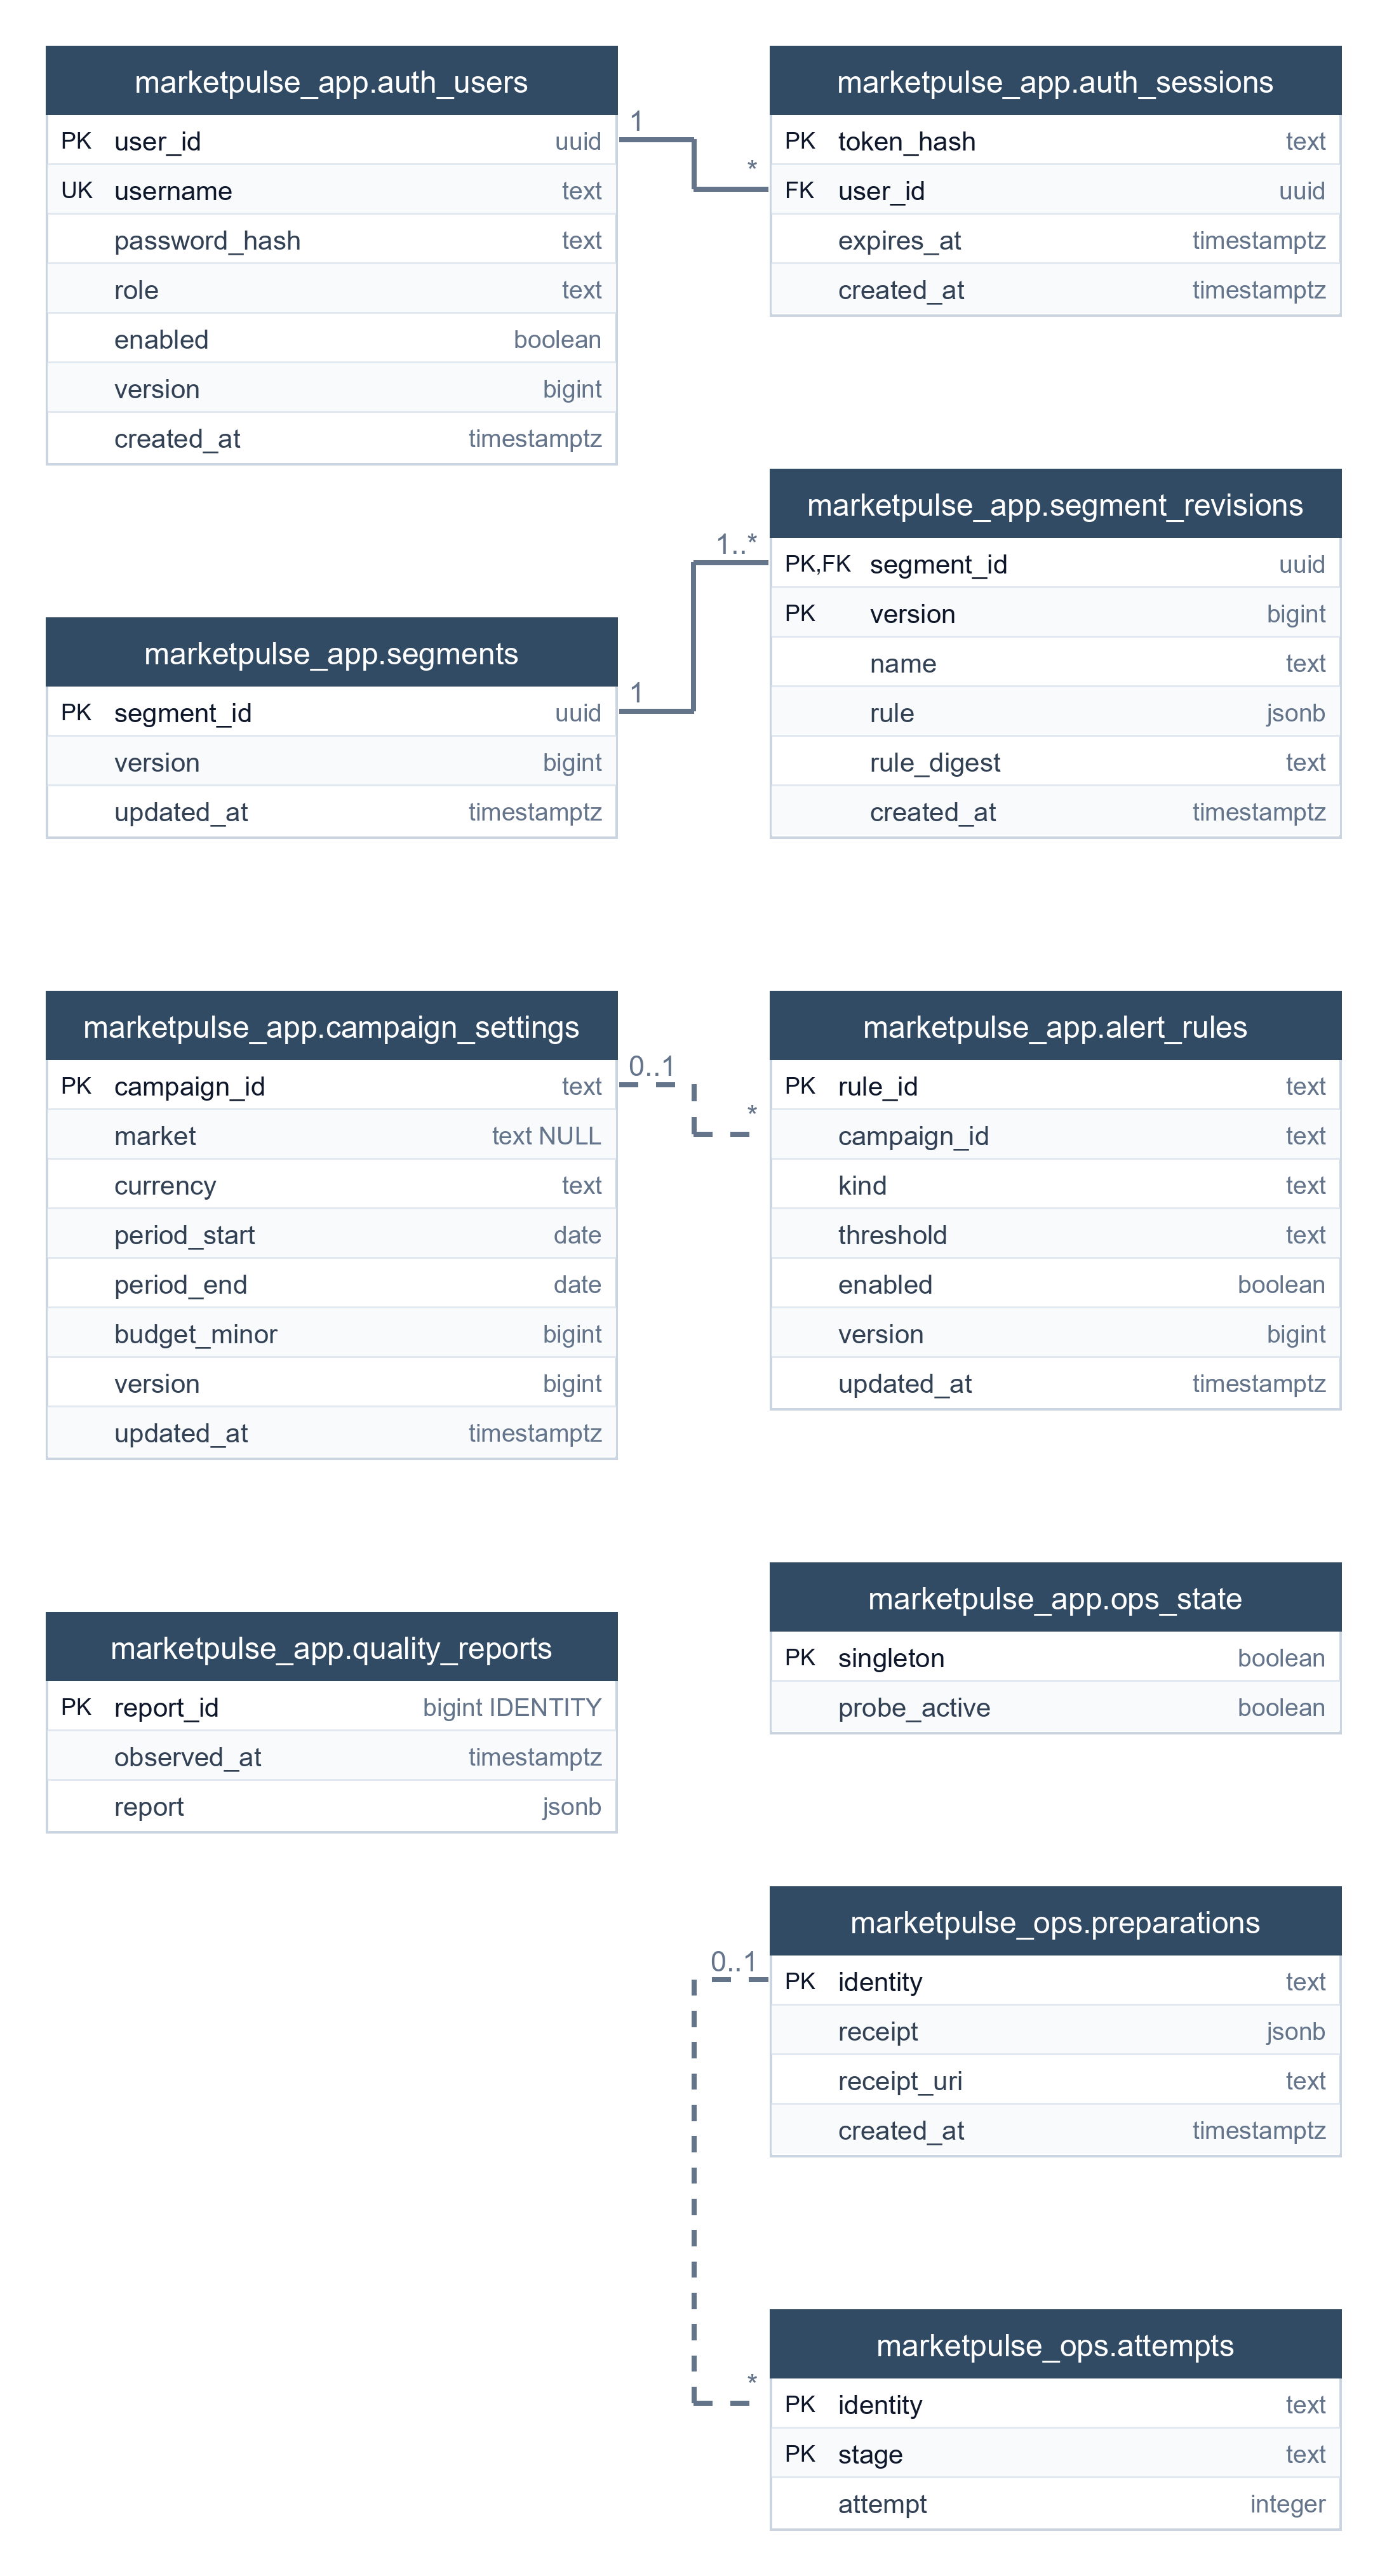
\includegraphics[width=\textwidth, height=0.88\textheight, keepaspectratio]{chapters/Pics/schema-postgres-1.png}
    \caption{Lược đồ quan hệ PostgreSQL (phần 1): tài khoản, phân đoạn, cấu hình chiến dịch, quy tắc cảnh báo và chuẩn bị công bố}
    \label{fig:schema-postgres}
\end{figure}

\begin{figure}[!htbp]
    \centering
    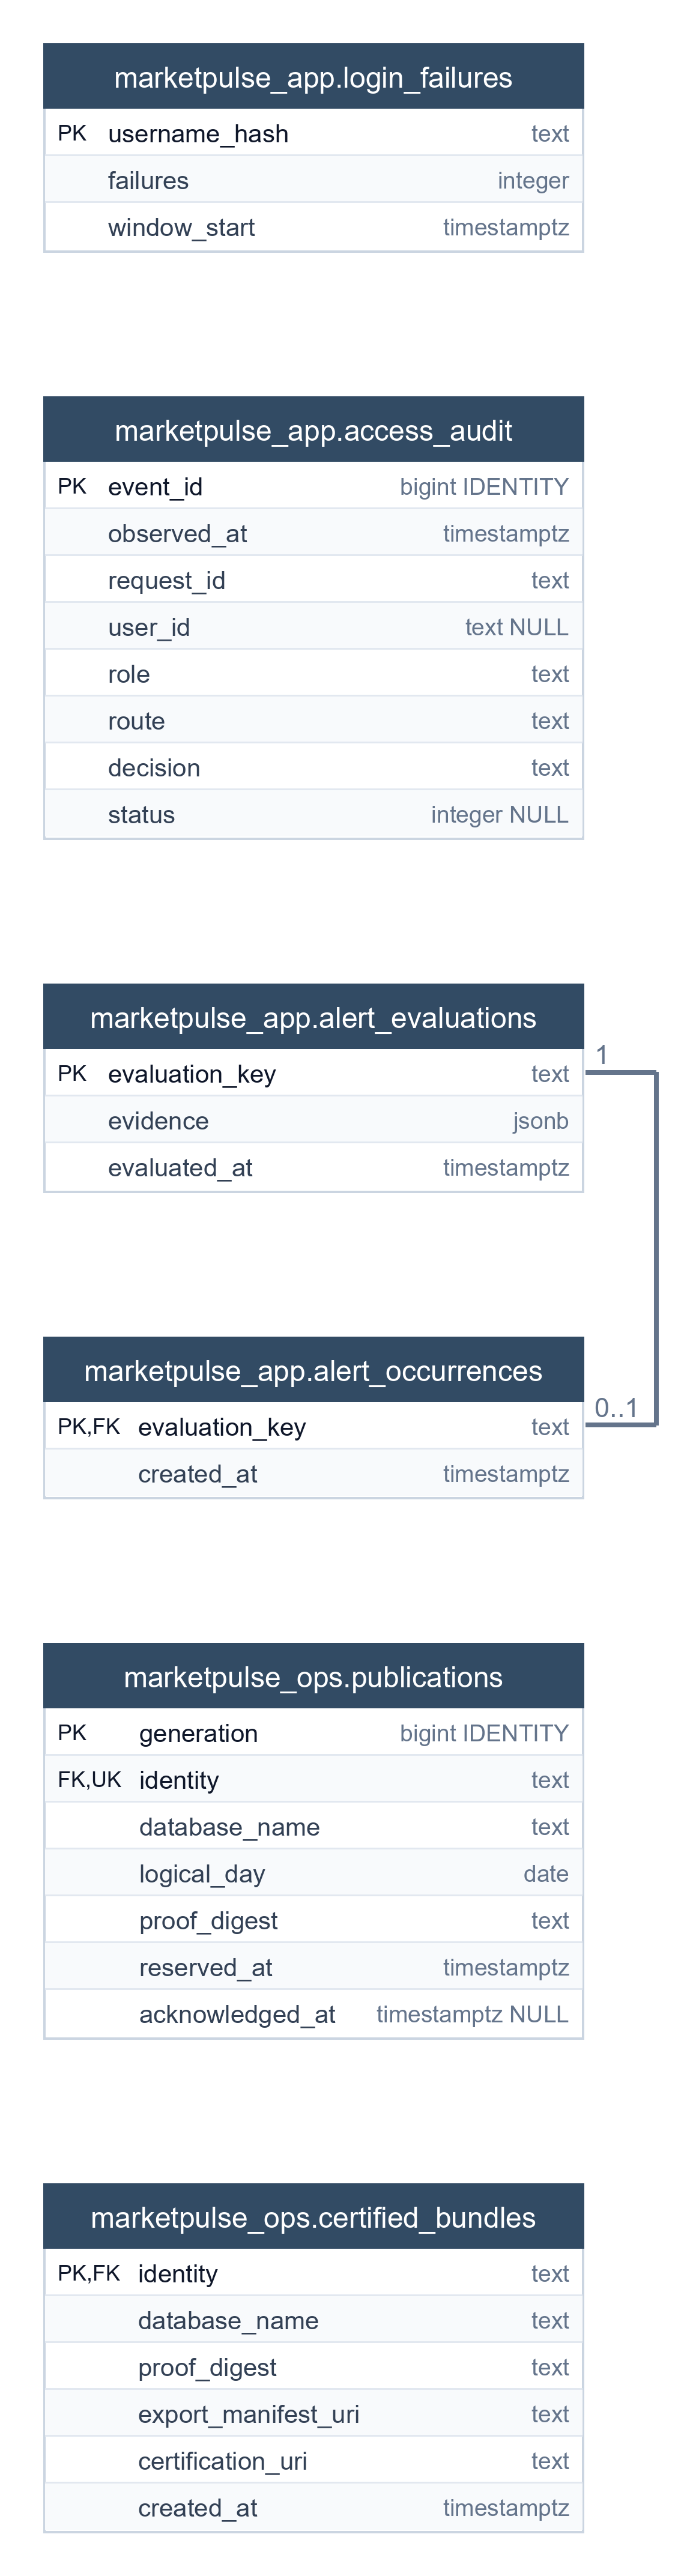
\includegraphics[width=\textwidth, height=0.88\textheight, keepaspectratio]{chapters/Pics/schema-postgres-2.png}
    \caption[Lược đồ quan hệ PostgreSQL (phần 2): kiểm toán truy cập, kết quả cảnh báo và sổ cái công bố]{Lược đồ quan hệ PostgreSQL (phần 2): kiểm toán truy cập, kết quả cảnh báo và sổ cái công bố. Khóa ngoại sang phần 1: \texttt{alert\_evaluations} tới \texttt{alert\_rules}; \texttt{publications} và \texttt{certified\_bundles} tới \texttt{preparations}}
    \label{fig:schema-postgres-2}
\end{figure}

\subsection{Các bảng phục vụ trên ClickHouse}
\label{sec:c4-clickhouse}
Ngoài các CSDL release, ClickHouse còn chứa ba nhóm bảng phục vụ ứng dụng (Hình~\ref{fig:schema-clickhouse} và Hình~\ref{fig:schema-clickhouse-2}). \texttt{marketpulse\_serving.publication\_journal} là nhật ký chỉ ghi thêm, phản chiếu bảng \texttt{publications} của sổ cái; \texttt{journey\_publications} ghi nhận CSDL hành trình của từng release. Trong CSDL sidecar, bảng \texttt{events} lưu hành trình đã ẩn danh và view \texttt{paid\_touches} chọn click trả phí đầu tiên cho mỗi cặp \texttt{(profile\_ref, click\_id)}. Kho \texttt{marketpulse\_live} gồm \texttt{campaign\_snapshots} (MergeTree), \texttt{events} (ReplacingMergeTree theo \texttt{(partition, offset)}) và hai bảng một dòng ghim định danh nguồn Kafka: nếu cụm Kafka hoặc topic bị thay đổi, worker từ chối ghi thay vì trộn hai nguồn.

\begin{figure}[!htbp]
    \centering
    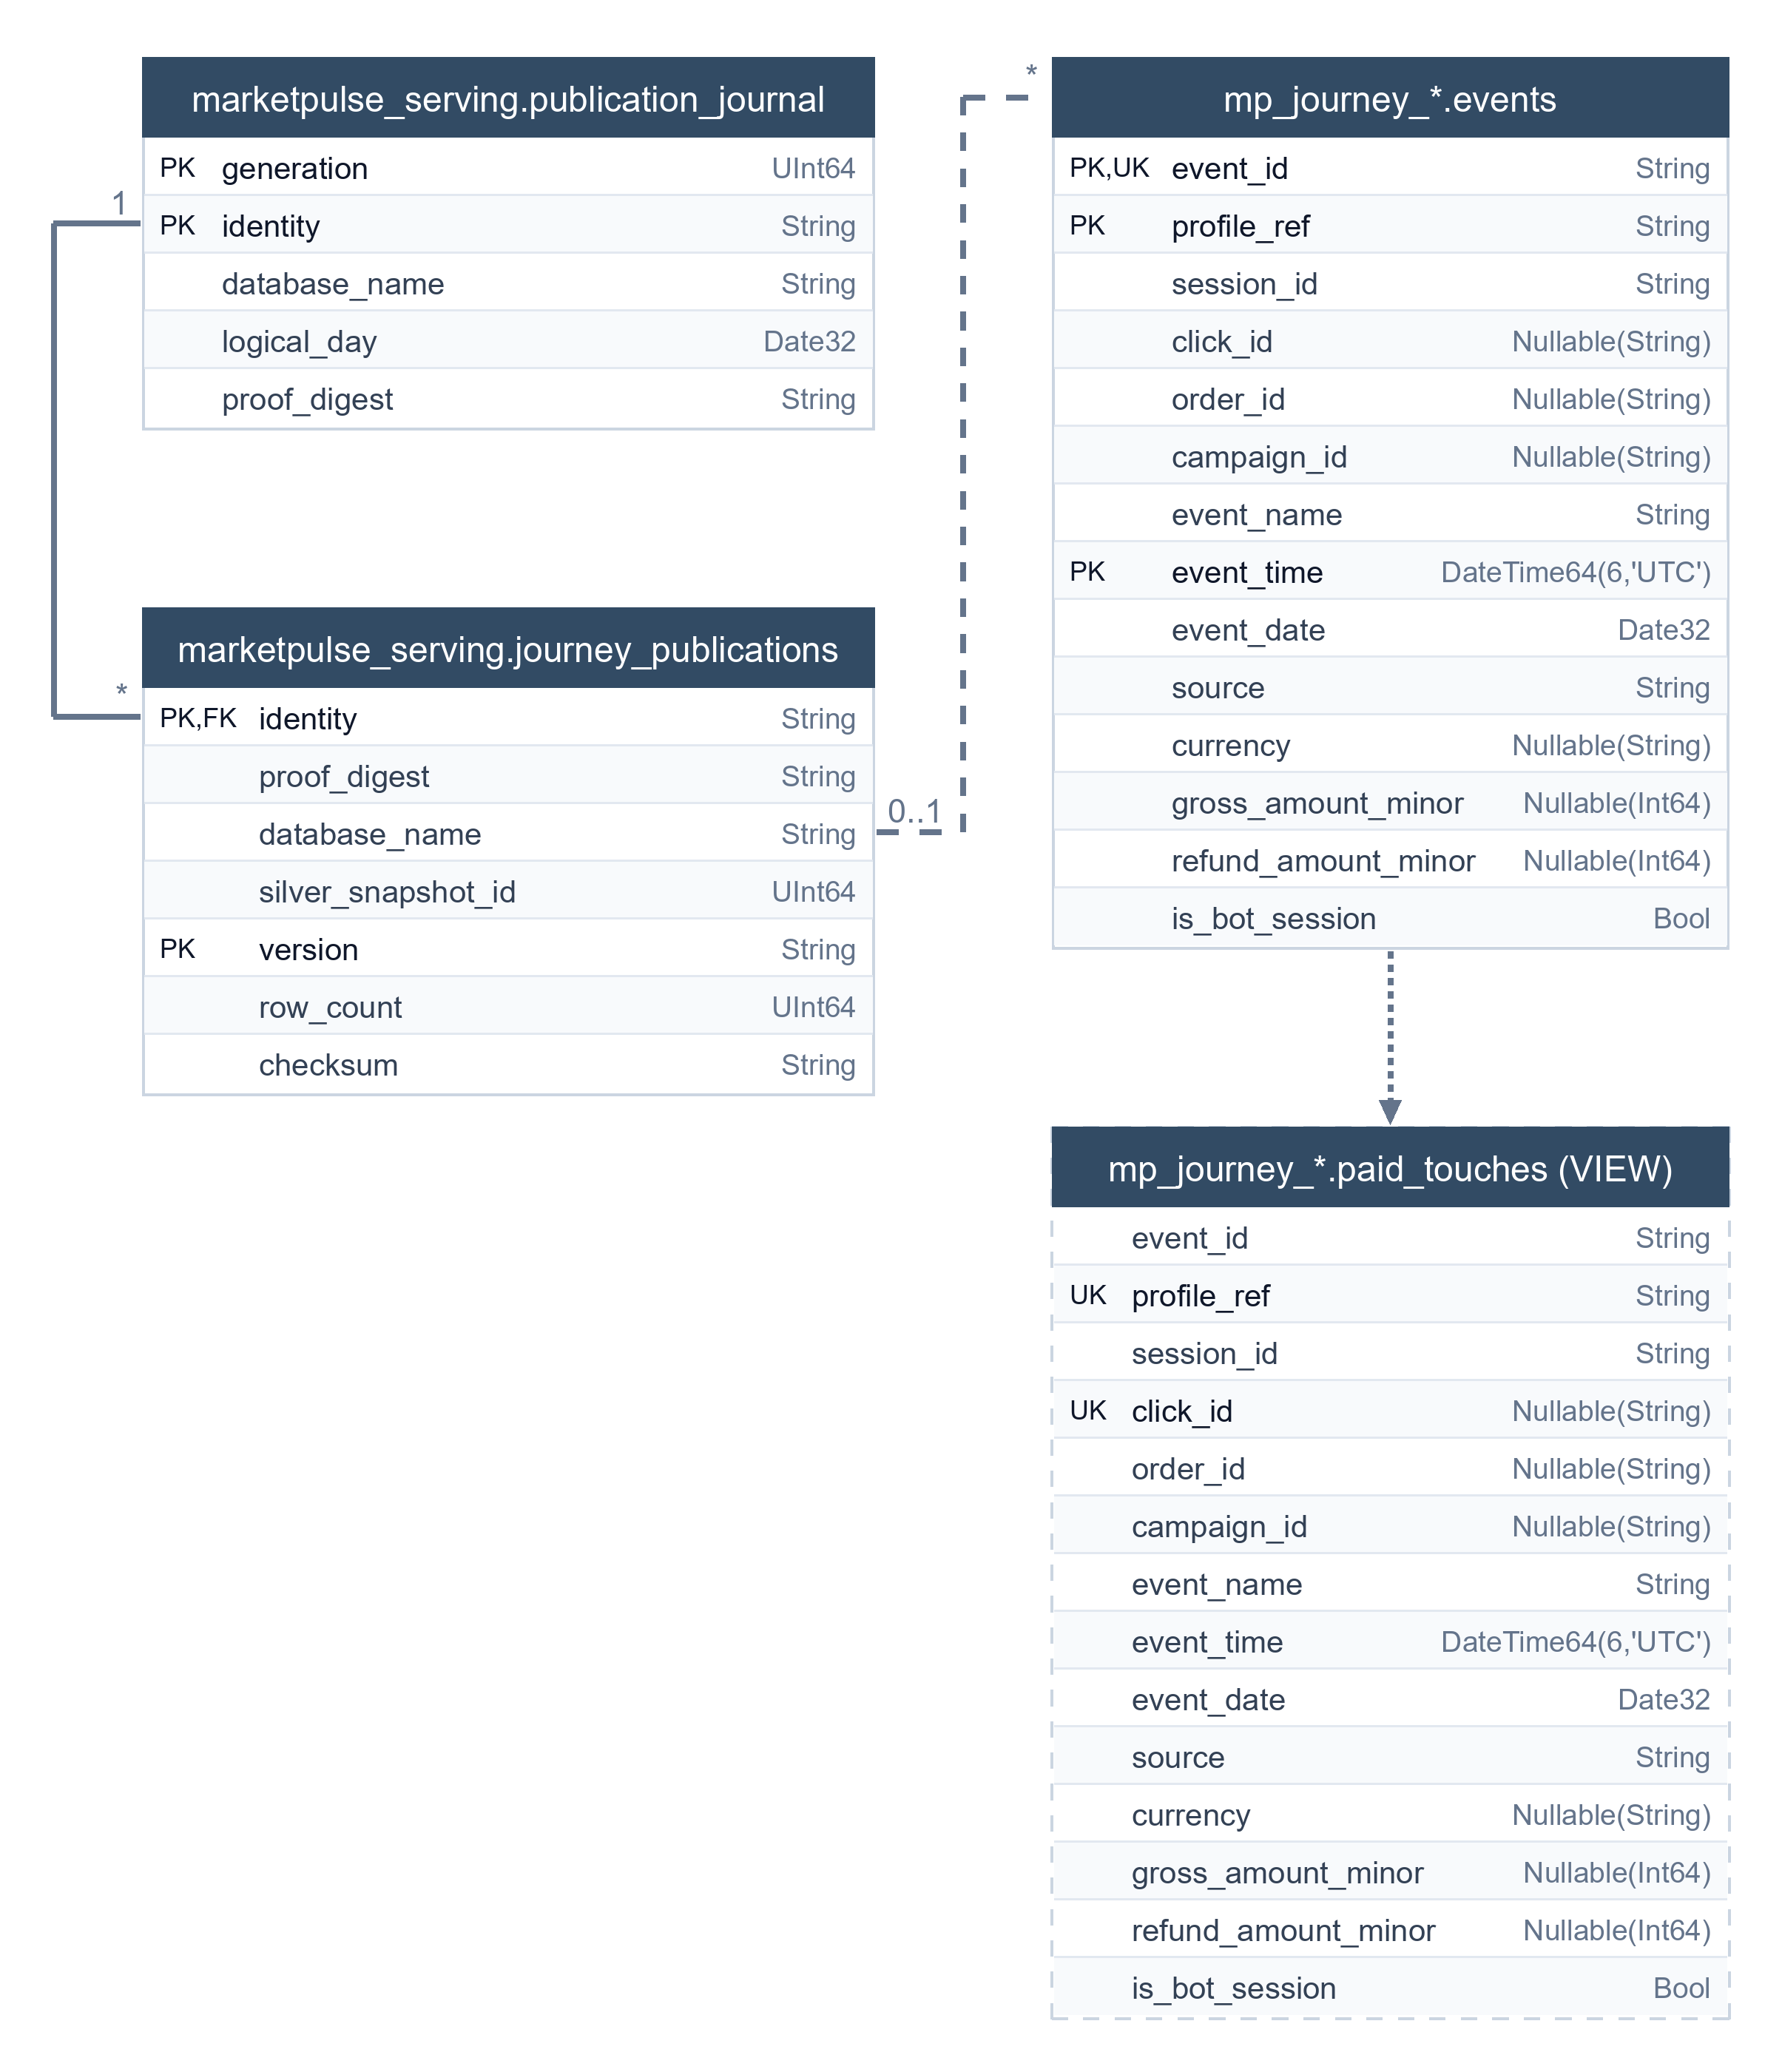
\includegraphics[width=\textwidth]{chapters/Pics/schema-clickhouse-1.png}
    \caption{Lược đồ quan hệ ClickHouse (phần 1): nhật ký công bố và CSDL hành trình (journey sidecar)}
    \label{fig:schema-clickhouse}
\end{figure}

\begin{figure}[!htbp]
    \centering
    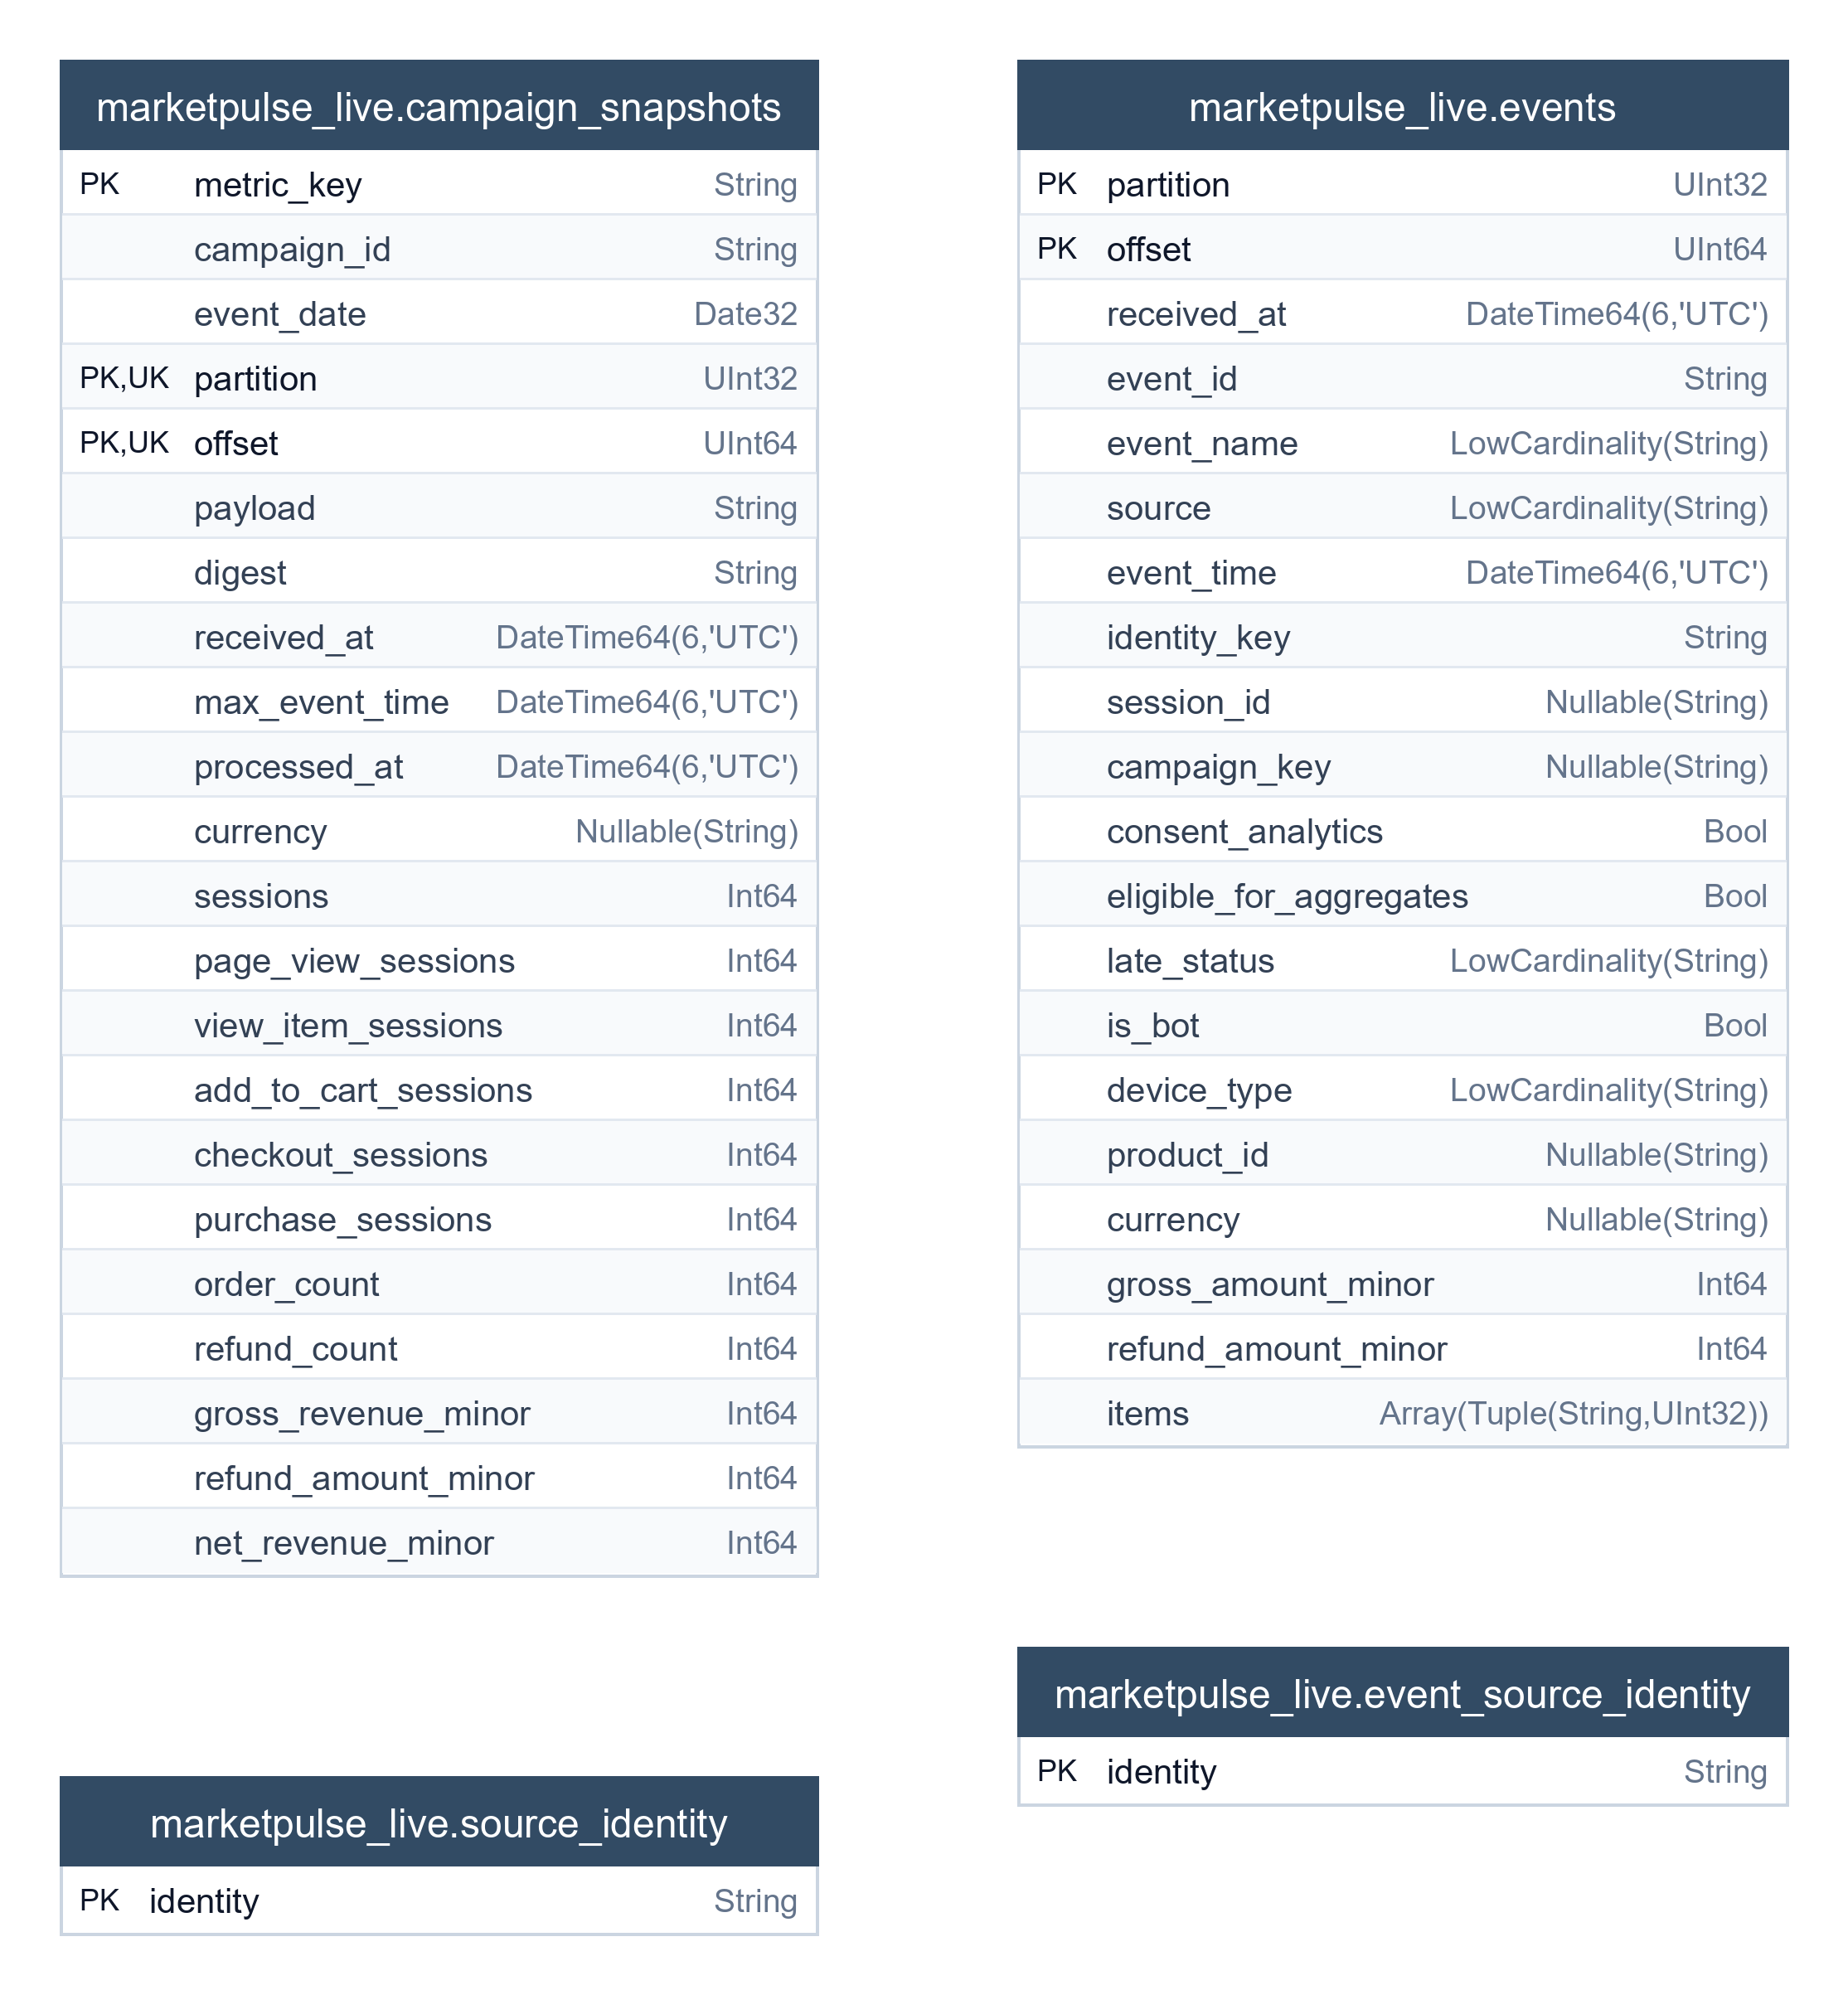
\includegraphics[width=0.92\textwidth]{chapters/Pics/schema-clickhouse-2.png}
    \caption{Lược đồ quan hệ ClickHouse (phần 2): kho dữ liệu trực tiếp \texttt{marketpulse\_live}}
    \label{fig:schema-clickhouse-2}
\end{figure}

\section{Giao diện và yêu cầu nghiệp vụ}
\label{sec:c4-giao-dien}

Kết quả trong phần này được đo trên release \texttt{109a2372\ldots} của bộ dữ liệu story-demo, gồm lịch sử đã kiểm chứng từ 01/01/2025 đến 31/08/2026 và luồng trực tiếp của tháng 09/2026. Mọi con số tổng hợp đều đã được một oracle độc lập tính lại từ file nguồn và khớp hoàn toàn (Mục~\ref{sec:c5-oracle}).

\subsection{Tổng quan giao diện}
\label{sec:c4-tong-quan-ui}
Giao diện được tổ chức thành 10 không gian làm việc, mỗi không gian phục vụ một nhóm câu hỏi (Bảng~\ref{tab:workspaces}). Nguyên tắc thiết kế xuyên suốt là \emph{trung thực về dữ liệu}: số liệu trực tiếp được gắn nhãn tạm thời và không bao giờ cộng với số liệu đã kiểm chứng; khi thiếu dữ liệu, giao diện hiển thị ``không có dữ liệu'' thay vì số 0; ngày tháng ghi rõ múi giờ.

\begin{table}[H]
\centering
\caption{Các không gian làm việc của Marketing Command Center}
\label{tab:workspaces}
\small
\renewcommand{\arraystretch}{1.2}
\begin{tabularx}{\textwidth}{>{\raggedright\arraybackslash}p{3.0cm} >{\raggedright\arraybackslash}p{2.2cm} >{\raggedright\arraybackslash}X}
\toprule
\textbf{Không gian} & \textbf{Đường dẫn} & \textbf{Nội dung chính} \\
\midrule
Overview & \texttt{/} & KPI chiến dịch đã kiểm chứng, số liệu trực tiếp, cảnh báo, giải ngân, mô phỏng \\
Live View & \texttt{/live} & Khách truy cập, phiên, đơn hàng của ngày hiện tại từ luồng trực tiếp \\
Ad Performance & \texttt{/ads} & Chi phí, click, ROAS theo nền tảng và chiến dịch \\
Analysis & \texttt{/analysis} & Phễu chuyển đổi, so sánh mô hình phân bổ, hành trình mẫu \\
Customers & \texttt{/customers} & Customer 360, dòng thời gian, phân đoạn, cohort, cơ hội và rủi ro \\
Email & \texttt{/email} & Số email đã gửi, đã nhận, được mở, được click, số lượt hủy đăng ký, số người nhận, tỷ lệ mở và click theo tháng \\
Insights & \texttt{/insights} & Nhịp hoạt động theo giờ, giá trị đơn hàng, kênh, khách hàng trung thành \\
Products & \texttt{/products} & Doanh thu theo ngành hàng và thiết bị \\
Geography & \texttt{/geography} & Doanh thu ròng theo 13 tỉnh/thành phố trên bản đồ Việt Nam \\
Data Health & \texttt{/operations} & Sức khỏe hệ thống, kiểm chứng chất lượng, lineage, kiểm toán \\
\bottomrule
\end{tabularx}
\end{table}

% Gợi ý: chèn ảnh chụp màn hình thật của từng không gian làm việc tại đây khi chạy story-demo, ví dụ:
% \begin{figure}[H]
%     \centering
%     \includegraphics[width=\textwidth]{chapters/Pics/ui-overview.png}
%     \caption{Màn hình Overview của Marketing Command Center}
%     \label{fig:ui-overview}
% \end{figure}

\subsection{Phân bổ doanh thu (BR-01)}
\label{sec:c4-br01}
Trong 20 tháng lịch sử, bốn nền tảng ghi nhận \num{2614669} lượt hiển thị, \num{227830} click và tổng chi phí \num{1339776177}~VND. Hình~\ref{fig:channels} đặt cạnh nhau tỷ trọng chi phí và tỷ trọng doanh thu gộp của từng nền tảng. Doanh thu ở đây được ghi nhận theo chiến dịch của click quảng cáo trả phí gắn trên chính đơn hàng (click của phiên mua hàng, hoặc click trả phí gần nhất trong 7 ngày trước đó), không theo mô hình First-Touch, Last-Touch hay Linear. Bốn nền tảng được ghi nhận tổng cộng \num{65,20}~tỷ VND trên \num{29059} đơn; \num{8,29}~tỷ VND còn lại (11,3\% doanh thu gộp, \num{3715} đơn) thuộc các đơn không có click trả phí nào trong 7 ngày trước khi mua nên không gắn với nền tảng nào. Shopee Ads chỉ chiếm 18,7\% chi phí nhưng mang về 31,5\% doanh thu gộp (\num{20,54}~tỷ VND từ \num{9158} đơn), trong khi Google Ads chiếm tỷ trọng chi phí lớn nhất (29,7\%) nhưng chỉ đóng góp 22,5\% doanh thu. Đây chính là loại phát hiện mà báo cáo riêng của từng nền tảng không thể đưa ra, và là cơ sở để \shCMO{} xem xét chuyển ngân sách. Trước khi quyết định, màn hình Analysis cho phép xem cùng phần doanh thu này được ba mô hình phân bổ ghi nhận khác nhau ra sao.

\begin{figure}[H]
\centering
\begin{tikzpicture}
\begin{axis}[
    name=left, xbar, width=0.43\textwidth, height=5.2cm, bar width=9pt,
    xmin=0, xmax=36, xlabel={Tỷ trọng chi phí (\%)},
    ytick={1,2,3,4}, yticklabels={Shopee,TikTok,Meta,Google}, 
    nodes near coords, nodes near coords align={horizontal},
    every node near coord/.append style={font=\scriptsize},
    tick label style={font=\footnotesize}, label style={font=\footnotesize},
    axis x line*=bottom, axis y line*=left, enlarge y limits=0.2]
  \addplot[fill=mphead, draw=mphead] coordinates {(29.7,4) (27.8,3) (23.8,2) (18.7,1)};
\end{axis}
\begin{axis}[
    at={(left.east)}, anchor=west, xshift=1.6cm,
    xbar, width=0.43\textwidth, height=5.2cm, bar width=9pt,
    xmin=0, xmax=36, xlabel={Tỷ trọng doanh thu gộp (\%)},
    ytick={1,2,3,4}, yticklabels={Shopee,TikTok,Meta,Google},
    nodes near coords, nodes near coords align={horizontal},
    every node near coord/.append style={font=\scriptsize},
    tick label style={font=\footnotesize}, label style={font=\footnotesize},
    axis x line*=bottom, axis y line*=left, enlarge y limits=0.2]
  \addplot[fill=mpaccent, draw=mpline] coordinates {(22.5,4) (25.6,3) (20.5,2) (31.5,1)};
\end{axis}
\end{tikzpicture}
\caption[Tỷ trọng chi phí và tỷ trọng doanh thu gộp theo nền tảng quảng cáo]{Tỷ trọng chi phí và tỷ trọng doanh thu gộp theo nền tảng quảng cáo, 01/2025 đến 08/2026. Doanh thu ghi nhận theo click trả phí gắn trên đơn hàng; mẫu số là \num{65,20}~tỷ VND doanh thu của bốn nền tảng}
\label{fig:channels}
\end{figure}

\subsection{Giám sát, cảnh báo và ngân sách (BR-02 -- BR-05)}
\label{sec:c4-br02-05}
Trong khi lịch sử dừng ở 31/08/2026, luồng tháng 09/2026 tiếp tục chảy vào màn hình Live View. Để kiểm tra số liệu trực tiếp có đáng tin hay không, nhóm đối chiếu màn hình với file nguồn tại cùng thời điểm phát lại (Bảng~\ref{tab:live-check}): sau khi khử trùng, lọc đồng thuận và loại phiên bot, hai bên khớp tuyệt đối.

\begin{table}[H]
\centering
\caption{Đối chiếu Live View với file nguồn tại thời điểm phát lại}
\label{tab:live-check}
\small
\renewcommand{\arraystretch}{1.2}
\begin{tabular}{lrr}
\toprule
\textbf{Chỉ số} & \textbf{Live View} & \textbf{File nguồn} \\
\midrule
Khách truy cập trong 30 phút gần nhất & 8 & 8 \\
Khách truy cập / phiên trong ngày & 224 / 231 & 224 / 231 \\
Đơn hàng & 25 & 25 \\
Doanh thu gộp (VND) & \num{60324000} & \num{60324000} \\
Hoàn tiền (VND) & \num{6805000} & \num{6805000} \\
Doanh thu ròng (VND) & \num{53519000} & \num{53519000} \\
\bottomrule
\end{tabular}
\end{table}

Cảnh báo (BR-03), giải ngân (BR-04) và mô phỏng (BR-05) cố ý dựa trên số liệu đã kiểm chứng của \texttt{campaign\_performance\_daily}, vì chi phí quảng cáo chỉ có ở nhánh lô. Ba loại quy tắc được hỗ trợ là vượt ngân sách, chi phí tăng đột biến so với ngày trước và tỷ trọng hoàn tiền; mỗi lần cảnh báo lưu kèm toán hạng, ngưỡng, cửa sổ thời gian và mã release làm bằng chứng. Phép mô phỏng tính doanh thu ròng dự kiến theo ROAS ròng lịch sử của từng chiến dịch và ghi rõ giả định ``kịch bản tuyến tính, không phải dự báo''.

\subsection{Kiểm chứng và sức khỏe hệ thống (BR-06)}
\label{sec:c4-br06}
Màn hình Data Health cho quản trị viên thấy release đang phục vụ, lineage từ snapshot Bronze đến \texttt{proof\_digest}, kết quả kiểm chứng lại toàn bộ bảng và đối soát tài chính, cùng nút chạy thử nghiệm làm hỏng có kiểm soát đã mô tả ở Ví dụ~4. Trên release story-demo, tổng doanh thu gộp \num{73488628000}~VND và hoàn tiền \num{4329091000}~VND khớp nhau giữa \texttt{commerce\_daily} và \texttt{campaign\_performance\_daily}, cho doanh thu ròng \num{69159537000}~VND trên \num{32774} đơn hàng.

\subsection{Phễu, Customer 360 và cohort (BR-07 -- BR-09)}
\label{sec:c4-br07-09}
Lớp hành trình gồm \num{298032} phiên web/app không phải bot. Kênh web có \num{198995} phiên với tỷ lệ chuyển đổi 11,9\%, ứng dụng có \num{99037} phiên với 8,5\%. Lưu lượng từ quảng cáo trả phí chiếm phần lớn (\num{219770} phiên xem trang), phần còn lại đến từ tìm kiếm tự nhiên, truy cập trực tiếp và email, chiếm 26,3\% số phiên sau quản trị. Nhịp hoạt động theo giờ Việt Nam cho thấy khung 20:00--22:00 có số phiên gấp 12,5 lần khung 02:00--04:00, cao điểm vào 21:00 thứ Bảy. Đây là thông tin hữu ích để lên lịch gửi email và chạy quảng cáo. Giá trị đơn hàng có trung vị \num{1797000}~VND và phân vị 90 là \num{4497000}~VND.

Ở góc độ sản phẩm (Hình~\ref{fig:products}), Thể thao và Làm đẹp dẫn đầu doanh thu gộp; máy tính để bàn và máy tính bảng tạo ra phần lớn doanh thu dù lưu lượng di động không nhỏ. Màn hình Customers cung cấp \num{748} dòng cohort theo tháng (các cohort từ 2023 đến 2026), hồ sơ Customer 360 với dòng thời gian hoạt động, phân đoạn RFM có lưu phiên bản và danh sách cơ hội như khách có nguy cơ rời bỏ (đã mua nhưng không quay lại từ 30 ngày) hoặc khách bỏ giỏ hàng.

\begin{figure}[H]
\centering
\begin{tikzpicture}
\begin{axis}[
    name=cat, xbar, width=0.43\textwidth, height=5.4cm, bar width=8pt,
    xmin=0, xmax=21, xlabel={Doanh thu gộp theo ngành hàng (tỷ VND)},
    ytick={1,2,3,4,5}, yticklabels={Thời trang,Gia dụng,Điện tử,Làm đẹp,Thể thao}, 
    nodes near coords, nodes near coords align={horizontal},
    every node near coord/.append style={font=\scriptsize},
    tick label style={font=\footnotesize}, label style={font=\footnotesize},
    axis x line*=bottom, axis y line*=left, enlarge y limits=0.15]
  \addplot[fill=mphead, draw=mphead] coordinates {(17.02,5) (16.74,4) (14.67,3) (12.90,2) (12.16,1)};
\end{axis}
\begin{axis}[
    at={(cat.east)}, anchor=west, xshift=1.9cm,
    xbar, width=0.43\textwidth, height=5.4cm, bar width=8pt,
    xmin=0, xmax=36, xlabel={Doanh thu gộp theo thiết bị (tỷ VND)},
    ytick={1,2,3,4}, yticklabels={Không rõ,Di động,Máy tính bảng,Máy tính}, 
    nodes near coords, nodes near coords align={horizontal},
    every node near coord/.append style={font=\scriptsize},
    tick label style={font=\footnotesize}, label style={font=\footnotesize},
    axis x line*=bottom, axis y line*=left, enlarge y limits=0.2]
  \addplot[fill=mpaccent, draw=mpline] coordinates {(29.45,4) (23.76,3) (18.94,2) (1.34,1)};
\end{axis}
\end{tikzpicture}
\caption{Doanh thu gộp đã kiểm chứng theo ngành hàng và theo thiết bị mua hàng}
\label{fig:products}
\end{figure}

Về địa lý (Hình~\ref{fig:geography}), TP.~Hồ Chí Minh và Hà Nội chiếm lần lượt 26,8\% và 25,0\% doanh thu ròng đã xác định vị trí. Khoảng \num{21,17}~tỷ VND đến từ hồ sơ ẩn danh hoặc chưa khớp được với khách hàng nên được tách riêng thành ``không xác định'' thay vì gán ngẫu nhiên cho một tỉnh thành; tổng các phần vẫn bằng đúng doanh thu ròng của Gold.

\begin{figure}[H]
\centering
\begin{tikzpicture}
\begin{axis}[
    xbar, width=0.82\textwidth, height=8.2cm, bar width=7pt,
    xmin=0, xmax=15, xlabel={Doanh thu ròng (tỷ VND)},
    ytick={1,2,3,4,5,6,7,8,9,10,11,12,13}, yticklabels={Hạ Long,Quy Nhơn,Huế,Buôn Ma Thuột,Vũng Tàu,Nha Trang,Hải Phòng,Biên Hòa,Đà Nẵng,Cần Thơ,Thủ Dầu Một,Hà Nội,TP. Hồ Chí Minh},
    nodes near coords, nodes near coords align={horizontal},
    every node near coord/.append style={font=\scriptsize},
    tick label style={font=\footnotesize}, label style={font=\footnotesize},
    axis x line*=bottom, axis y line*=left, enlarge y limits=0.05]
  \addplot[fill=mphead, draw=mphead] coordinates {
    (12.88,13) (12.02,12) (3.26,11) (2.82,10) (2.79,9)
    (2.74,8) (2.64,7) (1.77,6) (1.72,5) (1.42,4)
    (1.39,3) (1.36,2) (1.21,1)};
\end{axis}
\end{tikzpicture}
\caption{Doanh thu ròng đã kiểm chứng theo 13 tỉnh/thành phố (khách hàng đã xác định vị trí)}
\label{fig:geography}
\end{figure}

\subsection{Quyền riêng tư và tính lại lịch sử (BR-10)}
\label{sec:c4-br10}
Quản trị dữ liệu thể hiện trực tiếp trên số liệu: \num{1084} đơn hàng của khách từ chối đồng thuận phân tích không xuất hiện trong bất kỳ màn hình đã kiểm chứng nào. Hồ sơ trên giao diện chỉ hiện bút danh \texttt{profile\_ref}; phân đoạn chỉ được đánh dấu có thể kích hoạt khi khách hàng có đồng thuận marketing. Người dùng \texttt{viewer} không thấy và không gọi được các thao tác chi tiết hay vận hành; mọi quyết định truy cập nằm trong nhật ký kiểm toán. Việc tính lại lịch sử chạy cô lập qua \texttt{historical\_rebuild\_job} (Ví dụ~5) và không thay đổi release đang phục vụ.

\subsection{Tổng hợp đối chiếu yêu cầu}
\label{sec:c4-doi-chieu}
Bảng~\ref{tab:br-trace} truy vết mỗi yêu cầu nghiệp vụ tới màn hình, API và dữ liệu đã hiện thực.

\begin{table}[!htbp]
\centering
\caption{Truy vết yêu cầu nghiệp vụ tới màn hình, API (tiền tố \texttt{/api/v1}) và dữ liệu}
\label{tab:br-trace}
\footnotesize
\renewcommand{\arraystretch}{1.2}
\begin{tabularx}{\textwidth}{>{\raggedright\arraybackslash}p{1.1cm} >{\raggedright\arraybackslash}p{2.1cm} >{\raggedright\arraybackslash}p{6.0cm} >{\raggedright\arraybackslash}X}
\toprule
\textbf{BR} & \textbf{Màn hình} & \textbf{API chính} & \textbf{Dữ liệu} \\
\midrule
BR-01 & Analysis\newline Ads & \texttt{GET /analysis/attribution}\newline \texttt{GET /analysis/journeys} & \texttt{attribution\_daily}\newline \texttt{campaign\_performance\_daily}\newline \texttt{paid\_touches} \\
BR-02 & Overview\newline Live & \texttt{GET /dashboard}\newline \texttt{GET /live/view} & \texttt{marketpulse\_live.*} \\
BR-03 & Overview & \texttt{GET/POST /alert-rules}\newline \texttt{POST /alerts/evaluate} & \texttt{campaign\_performance\_daily}\newline bảng cảnh báo PostgreSQL \\
BR-04 & Overview & \texttt{GET /budget-pacing/\{campaign\_id\}} & \texttt{campaign\_settings}\newline \texttt{campaign\_performance\_daily} \\
BR-05 & Overview & \texttt{POST /budget-simulation} & \texttt{campaign\_performance\_daily} \\
BR-06 & Data Health & \texttt{POST /ops/quality/check}\newline \texttt{POST /ops/quality/probe} & release, \texttt{certified\_bundles}\newline \texttt{quality\_reports} \\
BR-07 & Analysis & \texttt{GET /analysis/funnel} & \texttt{funnel\_daily} \\
BR-08 & Customers\newline Email\newline Insights & \texttt{GET /lifecycle/profiles}\newline \texttt{GET /lifecycle/segments}\newline \texttt{GET /lifecycle/email-engagement}\newline \texttt{GET /insights/activity} & \texttt{customer\_360}\newline \texttt{mp\_journey\_*.events}\newline \texttt{segment\_revisions} \\
BR-09 & Customers\newline Products\newline Geography & \texttt{GET /lifecycle/cohorts}\newline \texttt{GET /insights/products}\newline \texttt{GET /insights/geography} & \texttt{cohort\_retention}\newline \texttt{commerce\_daily}\newline \texttt{customers} \\
BR-10 & Toàn bộ & \texttt{POST /auth/login}\newline \texttt{PUT /ops/users/\{id\}} & \texttt{auth\_*}, \texttt{access\_audit}\newline Silver đã quản trị \\
\bottomrule
\end{tabularx}
\end{table}


\newpage
\chapter{Đánh giá thực nghiệm}
\label{chap:danh-gia}
% =============================================================================
% CHƯƠNG 5 — ĐÁNH GIÁ THỰC NGHIỆM GIẢI PHÁP KỸ THUẬT DỮ LIỆU VÀ ỨNG DỤNG
% Số liệu lấy từ docs/evaluation/report.md, docs/runbooks/story-demo.md,
% docs/architecture/mp07-decisions.md, mp08-decisions.md (repo @ dbe614b).
% =============================================================================

Đề bài yêu cầu đánh giá giải pháp trên ba mặt: tính đúng đắn của dữ liệu sau xử lý, hiệu năng của giải pháp Kỹ thuật Dữ liệu, và hiệu quả hỗ trợ khai thác dữ liệu qua ứng dụng. Chương này định nghĩa trước các độ đo, sau đó trình bày kết quả của từng mặt. Mọi tiêu chí đều được định nghĩa bằng công thức hoặc bằng phép so sánh chính xác với một oracle độc lập.

\section{Môi trường và độ đo}
\label{sec:c5-moi-truong}

\subsection{Cấu hình môi trường thực nghiệm}
\label{sec:c5-cau-hinh}
Các thực nghiệm hiệu năng chạy trong một dự án Docker Compose cô lập (\texttt{compose.evaluation.yaml}) trên một máy với 15 CPU, 15,60~GiB bộ nhớ khả dụng, kiến trúc aarch64 và Docker Engine 29.4.0. Thực nghiệm xử lý luồng dùng Kafka 4.3.1 và Java 17, mỗi làn một partition, chu kỳ commit/checkpoint 1 giây cho cả hai động cơ. Thực nghiệm phục vụ phân tích giới hạn mỗi container CSDL ở 1,5~GiB bộ nhớ, tắt bộ nhớ đệm kết quả của ClickHouse, và chạy 20 lượt khởi động (warm-up) trước 100 lượt đo tuần tự cho mỗi truy vấn. Mỗi lượt đo luồng tạo một job hoặc ứng dụng mới. Các thực nghiệm hiệu năng là phép đo một lần trên máy cục bộ dùng chung, nên chỉ dùng để so sánh có kiểm soát giữa các phương án, không phải để suy ra năng lực sản xuất.

\subsection{Định nghĩa các độ đo}
\label{sec:c5-do-do}
Với $N$ bản ghi đầu vào, $t^{\mathrm{send}}_i$ là thời điểm bản ghi $i$ được gửi và $t^{\mathrm{obs}}_i$ là thời điểm kết quả tương ứng được quan sát thấy \emph{đã commit}:

\begin{itemize}
    \item \textbf{Thông lượng} (bản ghi/giây): $\displaystyle \mathit{TP} = \frac{N}{\max_i t^{\mathrm{obs}}_i - \min_i t^{\mathrm{send}}_i}$.
    \item \textbf{Độ trễ commit} của bản ghi $i$: $\ell_i = t^{\mathrm{obs}}_i - t^{\mathrm{send}}_i$, bao gồm thời gian xếp hàng và thời gian hiển thị giao dịch. Phân vị $p$ tính theo phương pháp \emph{nearest-rank}: $P_p = \ell_{(\lceil p \cdot n / 100 \rceil)}$ trên dãy $\ell$ đã sắp xếp tăng dần; báo cáo $P_{50}$, $P_{95}$, $P_{99}$.
    \item \textbf{Thời gian phục hồi}: $T_{\mathrm{rec}} = t_{\mathrm{out}} - t_{\mathrm{fail}}$, trong đó $t_{\mathrm{fail}}$ là lúc gây sự cố và $t_{\mathrm{out}}$ là lúc đầu ra mới đầu tiên được commit.
    \item \textbf{Thời gian CPU}: tổng mức tăng của bộ đếm CPU của các tiến trình liên quan trong cửa sổ đo; \textbf{bộ nhớ đỉnh}: giá trị lớn nhất của bộ nhớ làm việc được lấy mẫu.
    \item \textbf{Độ trễ truy vấn / API}: thời gian thực của một truy vấn hoặc một request HTTP có xác thực, báo cáo $P_{50}$, $P_{95}$, $P_{99}$ trên 100 mẫu.
    \item \textbf{Hệ số tăng tốc}: $S = P_{95}^{\mathrm{baseline}} / P_{95}^{\mathrm{candidate}}$.
    \item \textbf{Tính đúng đắn}: một phép kiểm tra \emph{đạt} khi giá trị của hệ thống bằng \emph{chính xác} giá trị của oracle độc lập. Số tiền là số nguyên nên sai số cho phép bằng 0.
\end{itemize}

\section{Tính đúng đắn của dữ liệu}
\label{sec:c5-dung-dan}

\subsection{Hệ thống kiểm thử tự động}
\label{sec:c5-kiem-thu}
Kho mã có 689 kiểm thử Python, 35 kiểm thử Java cho job Flink, 4 kiểm thử Java cho job đánh giá, 31 kiểm thử dữ liệu dbt và 20 file đặc tả kiểm thử giao diện bằng Playwright. Kiểm thử bao phủ toàn bộ đường ống: tính tất định của dữ liệu sinh, hợp đồng Kafka, thứ tự và tốc độ phát lại, khử trùng lặp, sự kiện trễ, phiên, chỉ số chiến dịch, quá trình nạp Bronze, quản trị Silver, các mô hình Gold, công bố và toàn bộ API. Ngoài kiểm thử đơn vị, các kịch bản Docker thật kiểm tra phục hồi sau sự cố, khởi động lại catalog/lưu trữ và dựng lại lịch sử cô lập.

Bảng~\ref{tab:test-results} ghi kết quả chạy thật của các bộ kiểm thử. Bộ kiểm thử Python được chạy lại ngày 13/11/2026 trên commit \texttt{dbe614b}, môi trường Linux (WSL2) với Python 3.12.11: 641 kiểm thử đạt, 41 kiểm thử bỏ qua và 7 kiểm thử không đạt. 41 kiểm thử bỏ qua là kiểm thử tích hợp, chỉ chạy khi được bật bằng biến môi trường và có PostgreSQL, ClickHouse, Dagster hoặc Spark thật. Cả 7 kiểm thử không đạt đều gọi lệnh \texttt{docker compose config} để kiểm tra file cấu hình Compose và thất bại vì máy chạy kiểm thử không có Docker Engine đang hoạt động, không phải do lỗi logic của hệ thống. 31 kiểm thử dbt đều đạt trong lần kiểm chứng release story-demo (lượt chạy \texttt{2d216b87}), vì quy trình công bố dừng ngay khi \texttt{dbt build} có kiểm thử thất bại. Các kiểm thử Java và Playwright chưa được chạy lại trong khuôn khổ báo cáo này.

\begin{table}[H]
\centering
\caption{Kết quả chạy các bộ kiểm thử tự động}
\label{tab:test-results}
\small
\renewcommand{\arraystretch}{1.2}
\begin{tabularx}{\textwidth}{>{\raggedright\arraybackslash}p{4.6cm} >{\raggedleft\arraybackslash}p{2.1cm} >{\raggedright\arraybackslash}X}
\toprule
\textbf{Bộ kiểm thử} & \textbf{Số lượng} & \textbf{Kết quả} \\
\midrule
Python (\texttt{unittest}, Linux, 13/11/2026) & 689 & 641 đạt, 41 bỏ qua (tích hợp), 7 không đạt (cần Docker Engine) \\
dbt (release story-demo \texttt{2d216b87}) & 31 & 31 đạt \\
Java, job Flink & 35 & Chưa chạy lại \\
Java, job đánh giá & 4 & Chưa chạy lại \\
Playwright, giao diện & 20 file & Chưa chạy lại \\
\bottomrule
\end{tabularx}
\end{table}

\subsection{Đối soát độc lập trên story-demo}
\label{sec:c5-oracle}
Script \texttt{story\_demo\_oracle.py} tính lại các chỉ số từ chính file nguồn của bộ sinh (không qua đường ống) rồi so với dữ liệu của hệ thống: 322 phép kiểm tra so với release đã kiểm chứng trên ClickHouse và 64 phép kiểm tra so với tầng Silver, đọc qua Spark. Kết quả: \textbf{386/386 phép kiểm tra bằng nhau} (Bảng~\ref{tab:correctness}). Chênh lệch duy nhất giữa dữ liệu thô và dữ liệu đã kiểm chứng được giải thích trọn vẹn bởi quản trị: \num{33858} đơn hàng thô so với \num{32774} đơn đã kiểm chứng, chênh đúng \num{1084} đơn hàng không có đồng thuận phân tích.

\begin{table}[H]
\centering
\caption{Kết quả đối soát tính đúng đắn của dữ liệu}
\label{tab:correctness}
\small
\renewcommand{\arraystretch}{1.2}
\begin{tabularx}{\textwidth}{>{\raggedright\arraybackslash}p{3.6cm} >{\raggedright\arraybackslash}X >{\raggedright\arraybackslash}p{3.2cm}}
\toprule
\textbf{Tập dữ liệu} & \textbf{Phép kiểm tra} & \textbf{Kết quả} \\
\midrule
Fixture & Doanh thu gộp \num{27160000}, hoàn \num{4967000}, ròng \num{22193000} VND bảo toàn qua cả ba mô hình phân bổ & Khớp tuyệt đối \\
Story-demo (release) & Hiển thị, click, chi phí của 4 nền tảng $\times$ 20 tháng & 240/240 \\
Story-demo (release) & Đơn hàng, doanh thu gộp, hoàn tiền theo tháng (60); đơn hàng và doanh thu gộp theo nền tảng của click trên đơn hàng (8); doanh thu theo 13 tỉnh/thành và nhóm ẩn danh (14) & 82/82 \\
Story-demo (Silver) & Số email đã gửi theo loại $\times$ tháng (60); phiên theo nguồn truy cập sau quản trị (4) & 64/64 \\
Live View & Khách truy cập, phiên, đơn hàng, doanh thu so với file nguồn tại cùng thời điểm phát lại & Khớp tuyệt đối \\
Evaluation 10k/100k & Mỗi đầu ra đã commit so với oracle Python; mã băm chuẩn hóa đầu vào/đầu ra giữa Flink và Kafka Streams & Khớp ở cả hai quy mô \\
\bottomrule
\end{tabularx}
\end{table}

\subsection{Đối chiếu đầu ra Flink và Kafka Streams}
\label{sec:c5-tuong-duong}
Trước khi so sánh tốc độ, hai động cơ phải cho cùng một kết quả. Khối lượng công việc tài chính tất định gồm cả bản ghi trùng, bản ghi sai giá trị, bản ghi trễ trong ngưỡng và trễ quá ngưỡng. Với mỗi đầu ra đã commit, một oracle Python độc lập kiểm tra tính đầy đủ của chuỗi, cách phân loại và số tiền trung gian theo từng chiến dịch. Kết quả xác nhận: bản ghi trùng không làm thay đổi tổng, giá trị sai không làm sai lệch số tiền, bản ghi trễ trong ngưỡng được tính và bản ghi trễ quá ngưỡng được ghi nhận rồi loại ra. Mã băm chuẩn hóa của đầu vào và đầu ra giống nhau giữa hai động cơ.

\section{Flink và Kafka Streams}
\label{sec:c5-flink-vs-streams}

\subsection{Thông lượng và độ trễ}
\label{sec:c5-thong-luong}
Bảng~\ref{tab:flink-streams} và Hình~\ref{fig:flink-streams} cho thấy kết quả phụ thuộc rõ vào quy mô. Ở \texttt{eval-medium} (\num{100000} sự kiện), Flink đạt \num{79812.6} bản ghi/giây, gấp 1,53 lần Kafka Streams (\num{52039.8}), và độ trễ $P_{95}$ thấp hơn 33,6\% (\num{1094.34} ms so với \num{1648.05} ms). Ngược lại, ở \texttt{eval-small} (\num{10000} sự kiện), Kafka Streams nhanh hơn với \num{11394.2} bản ghi/giây và $P_{95}$ \num{858.45} ms so với \num{7887.2} bản ghi/giây và \num{1240.90} ms của Flink. Đây là kết quả hợp lý: Kafka Streams là thư viện nhúng nên khởi động nhẹ, phù hợp với tải nhỏ; khi tải tăng, động cơ phân tán của Flink mới phát huy lợi thế. Độ trễ ở đây bao gồm cả thời gian hiển thị giao dịch với chu kỳ commit 1 giây, nên không phải độ trễ từ sự kiện đến bảng điều khiển trong vận hành thực tế.

\begin{table}[H]
\centering
\caption{Thông lượng và độ trễ commit của Apache Flink 2.2.1 và Kafka Streams 4.3.1}
\label{tab:flink-streams}
\small
\renewcommand{\arraystretch}{1.2}
\begin{tabular}{llrrrr}
\toprule
\textbf{Động cơ} & \textbf{Quy mô} & \textbf{Bản ghi/giây} & \textbf{$P_{50}$ (ms)} & \textbf{$P_{95}$ (ms)} & \textbf{$P_{99}$ (ms)} \\
\midrule
Flink & eval-small (10k) & \num{7887.2} & \num{1133.39} & \num{1240.90} & \num{1242.23} \\
Kafka Streams & eval-small (10k) & \num{11394.2} & \num{852.90} & \num{858.45} & \num{858.76} \\
Flink & eval-medium (100k) & \num{79812.6} & \num{1085.17} & \num{1094.34} & \num{1096.43} \\
Kafka Streams & eval-medium (100k) & \num{52039.8} & \num{1635.03} & \num{1648.05} & \num{1651.72} \\
\bottomrule
\end{tabular}
\end{table}

\begin{figure}[H]
\centering
\begin{tikzpicture}
\begin{axis}[
    name=tp, ybar, width=0.47\textwidth, height=5.6cm, bar width=12pt,
    ymin=0, ymax=95000, ylabel={Bản ghi/giây},
    xtick={1,2}, xticklabels={10k sự kiện,100k sự kiện}, xmin=0.5, xmax=2.5,
    legend style={at={(0.5,1.03)}, anchor=south, legend columns=2, font=\scriptsize, draw=none, /tikz/every even column/.append style={column sep=6pt}},
    nodes near coords, every node near coord/.append style={font=\tiny, rotate=90, anchor=west},
    tick label style={font=\footnotesize}, label style={font=\footnotesize},
    scaled y ticks=false, yticklabel style={/pgf/number format/fixed},
    axis x line*=bottom, axis y line*=left]
  \addplot[fill=mphead, draw=mphead] coordinates {(1,7887.2) (2,79812.6)};
  \addplot[fill=mpaccent, draw=mpline] coordinates {(1,11394.2) (2,52039.8)};
  \legend{Flink, Kafka Streams}
\end{axis}
\begin{axis}[
    at={(tp.east)}, anchor=west, xshift=1.8cm,
    ybar, width=0.36\textwidth, height=5.6cm, bar width=22pt,
    ymin=0, ymax=55, ylabel={Thời gian phục hồi (giây)},
    xtick={1,2}, xticklabels={Flink,Kafka Streams}, xmin=0.4, xmax=2.6,
    nodes near coords, every node near coord/.append style={font=\scriptsize},
    tick label style={font=\footnotesize}, label style={font=\footnotesize},
    axis x line*=bottom, axis y line*=left]
  \addplot[fill=mphead, draw=mphead] coordinates {(1,4.48)};
  \addplot[fill=mpaccent, draw=mpline, bar shift=0pt] coordinates {(2,45.28)};
\end{axis}
\end{tikzpicture}
\caption{Thông lượng theo quy mô và thời gian phục hồi sau sự cố của Flink và Kafka Streams}
\label{fig:flink-streams}
\end{figure}

\subsection{Thời gian phục hồi sau sự cố}
\label{sec:c5-phuc-hoi}
Khi tiến trình xử lý bị dừng đột ngột ở quy mô \texttt{eval-small}, Flink khôi phục từ checkpoint số 4 và có đầu ra mới được commit sau \num{4.476} giây. Kafka Streams giữ nguyên application ID và trạng thái cục bộ nhưng phải phát lại changelog của trạng thái, mất \num{45.277} giây, chậm hơn khoảng 10,1 lần. Với nhánh luồng của MarketPulse 360, nơi trạng thái gồm khử trùng lặp 7 ngày, phiên và chỉ số chiến dịch, khả năng phục hồi nhanh là yếu tố quyết định. Kết hợp với lợi thế ở tải lớn và các tính năng thời gian sự kiện, kết quả củng cố lựa chọn Flink làm động cơ chính. Cần lưu ý phạm vi so sánh: đây là một bộ tổng hợp tài chính giới hạn, chưa bao gồm gom phiên, toàn bộ xử lý hợp đồng và TTL trạng thái của job thật.

\section{ClickHouse và PostgreSQL}
\label{sec:c5-clickhouse-vs-postgres}

\subsection{Độ trễ truy vấn theo quy mô}
\label{sec:c5-do-tre-truy-van}
Hai hệ thống được nạp cùng một bảng dữ liệu mô phỏng gồm năm cột, sinh tuần hoàn với 64 chiến dịch, 30 ngày và 3 nền tảng, tiền là số nguyên. Bảng có cấu trúc giống tầng Gold nhưng không phải dữ liệu story-demo. Thực nghiệm dùng ba quy mô 1, 10 và 20 triệu dòng và ba truy vấn đại diện: tổng theo nền tảng (\texttt{platform}), tổng theo chiến dịch và ngày (\texttt{campaign\_day}), và truy vấn lọc theo chiến dịch trong một khoảng ngày (\texttt{filtered}). Điều kiện so sánh như sau. PostgreSQL 17.6 dùng cấu hình mặc định của image (\texttt{shared\_buffers} 128~MB), \texttt{max\_parallel\_workers\_per\_gather = 1} và một chỉ mục B-tree trên \texttt{(campaign, event\_day)} tạo sau khi nạp, kèm lệnh \texttt{ANALYZE}; bảng không được sắp xếp lại bằng \texttt{CLUSTER}, không có chỉ mục bao phủ và không phân vùng. ClickHouse dùng động cơ MergeTree với khóa sắp xếp \texttt{(campaign, event\_day, row\_id)}, \texttt{max\_threads = 2} và tắt bộ nhớ đệm truy vấn. Mọi lượt đo đều trả về đúng đáp án của oracle.

\begin{table}[H]
\centering
\caption{Độ trễ truy vấn (ms) của ClickHouse 26.8 và PostgreSQL 17.6}
\label{tab:ch-pg}
\small
\renewcommand{\arraystretch}{1.15}
\begin{tabular}{llrrrrrr}
\toprule
 & & \multicolumn{3}{c}{\textbf{ClickHouse}} & \multicolumn{3}{c}{\textbf{PostgreSQL}} \\
\cmidrule(lr){3-5}\cmidrule(lr){6-8}
\textbf{Quy mô} & \textbf{Truy vấn} & $P_{50}$ & $P_{95}$ & $P_{99}$ & $P_{50}$ & $P_{95}$ & $P_{99}$ \\
\midrule
1M & filtered & \num{1.93} & \num{2.86} & \num{3.11} & \num{2.53} & \num{3.28} & \num{3.87} \\
1M & platform & \num{7.13} & \num{11.04} & \num{12.22} & \num{32.03} & \num{38.43} & \num{49.69} \\
1M & campaign\_day & \num{10.98} & \num{16.12} & \num{18.08} & \num{37.06} & \num{43.22} & \num{45.25} \\
\midrule
10M & filtered & \num{3.60} & \num{4.47} & \num{5.22} & \num{88.86} & \num{109.82} & \num{158.55} \\
10M & platform & \num{47.88} & \num{53.59} & \num{54.39} & \num{333.15} & \num{422.23} & \num{617.17} \\
10M & campaign\_day & \num{71.06} & \num{82.23} & \num{86.73} & \num{389.00} & \num{518.30} & \num{583.10} \\
\midrule
20M & filtered & \num{4.28} & \num{5.02} & \num{5.29} & \num{378.42} & \num{518.54} & \num{651.49} \\
20M & platform & \num{98.07} & \num{109.05} & \num{122.08} & \num{740.74} & \num{826.55} & \num{1074.45} \\
20M & campaign\_day & \num{148.52} & \num{196.89} & \num{221.05} & \num{849.06} & \num{977.09} & \num{1298.05} \\
\bottomrule
\end{tabular}
\end{table}

Ở 1 triệu dòng, hai hệ thống gần như ngang nhau với truy vấn có chỉ mục (2,86 ms so với 3,28 ms). Khoảng cách nới rộng nhanh khi dữ liệu tăng (Hình~\ref{fig:ch-pg}): ở 20 triệu dòng, ClickHouse nhanh hơn 103,3 lần với \texttt{filtered} (5,02 ms so với 518,54 ms), 7,58 lần với \texttt{platform} và 4,96 lần với \texttt{campaign\_day} xét theo $P_{95}$. Nguyên nhân chính nằm ở cách lưu trữ: ClickHouse chỉ đọc các cột cần thiết và bỏ qua các khối dữ liệu không thỏa điều kiện nhờ khóa sắp xếp, trong khi PostgreSQL đọc cả dòng. Riêng mức chênh 103 lần ở \texttt{filtered} còn đến từ thứ tự vật lý của dữ liệu: ClickHouse lưu các dòng của cùng một chiến dịch liền nhau, còn ở PostgreSQL các dòng thỏa điều kiện nằm rải khắp bảng vì dữ liệu được nạp theo thứ tự \texttt{row\_id}, nên dù có chỉ mục vẫn phải đọc gần như mọi trang dữ liệu. Phương án PostgreSQL có \texttt{CLUSTER} theo chỉ mục hoặc có chỉ mục bao phủ chưa được thử, nên kết luận này chỉ áp dụng cho cấu hình PostgreSQL đã nêu.

\begin{figure}[H]
\centering
\begin{tikzpicture}
\begin{axis}[
    name=lat, ybar, ymode=log, width=0.5\textwidth, height=5.8cm, bar width=10pt,
    ymin=1, ymax=3000, ylabel={$P_{95}$ ở 20M dòng (ms, thang log)},
    xtick={1,2,3}, xticklabels={filtered,platform,campaign\_day}, xmin=0.5, xmax=3.5,
    legend style={at={(0.5,1.03)}, anchor=south, legend columns=2, font=\scriptsize, draw=none, /tikz/every even column/.append style={column sep=6pt}},
    nodes near coords, every node near coord/.append style={font=\tiny},
    tick label style={font=\footnotesize}, label style={font=\footnotesize},
    axis x line*=bottom, axis y line*=left, log origin=infty]
  \addplot[fill=mphead, draw=mphead] coordinates {(1,5.02) (2,109.05) (3,196.89)};
  \addplot[fill=mpaccent, draw=mpline] coordinates {(1,518.54) (2,826.55) (3,977.09)};
  \legend{ClickHouse, PostgreSQL}
\end{axis}
\begin{axis}[
    at={(lat.east)}, anchor=west, xshift=1.8cm,
    ybar, width=0.42\textwidth, height=5.8cm, bar width=10pt,
    ymin=0, ymax=620, ylabel={Thời gian CPU (giây)},
    xtick={1,2,3}, xticklabels={1M,10M,20M}, xmin=0.5, xmax=3.5,
    legend style={at={(0.5,1.03)}, anchor=south, legend columns=2, font=\scriptsize, draw=none, /tikz/every even column/.append style={column sep=6pt}},
    nodes near coords, every node near coord/.append style={font=\tiny, rotate=90, anchor=west},
    tick label style={font=\footnotesize}, label style={font=\footnotesize},
    axis x line*=bottom, axis y line*=left]
  \addplot[fill=mphead, draw=mphead] coordinates {(1,2.62) (2,15.37) (3,32.75)};
  \addplot[fill=mpaccent, draw=mpline] coordinates {(1,16.94) (2,196.61) (3,485.16)};
  \legend{ClickHouse, PostgreSQL}
\end{axis}
\end{tikzpicture}
\caption{Độ trễ truy vấn $P_{95}$ ở 20 triệu dòng và thời gian CPU theo quy mô của ClickHouse và PostgreSQL}
\label{fig:ch-pg}
\end{figure}

\subsection{Mức tiêu thụ tài nguyên}
\label{sec:c5-tai-nguyen}
Trong cùng khối lượng truy vấn, PostgreSQL tiêu tốn \num{485.16} giây CPU ở 20 triệu dòng, so với \num{32.75} giây của ClickHouse, tức tiết kiệm khoảng 14,8 lần. Đổi lại, ClickHouse dùng nhiều bộ nhớ hơn (đỉnh khoảng 1~GiB so với \num{534.2}~MiB của PostgreSQL) do xử lý theo khối cột lớn. Kết quả xác nhận cách phân công trong kiến trúc: ClickHouse cho truy vấn phân tích, PostgreSQL cho dữ liệu vận hành cần ràng buộc và giao dịch. Phương án Google BigQuery/BigLake không được đo nên không có kết luận về phương án này.

\section{Thời gian chạy nhánh lô}
\label{sec:c5-batch-runtime}

Nhánh lô được đo trên story-demo trong một lần chạy ngày 03/11/2026, trên một máy cục bộ có 24~GB bộ nhớ, khác với máy dùng cho các thực nghiệm ở trên; Spark driver được cấp 5~GB và ClickHouse được giới hạn 4~GiB bộ nhớ. Bảng~\ref{tab:batch-runtime} ghi thời gian thực của ba công đoạn chính. Job hằng ngày cho một ngày dữ liệu hoàn tất trong chưa tới 10 phút, đủ để chạy theo lịch lúc 02:00 và công bố số liệu trước giờ làm việc. Đây là phép đo một lần, chưa cho biết thời gian chạy khi khối lượng dữ liệu lớn hơn.

\begin{table}[H]
\centering
\caption{Thời gian chạy các công đoạn chính của nhánh lô trên story-demo}
\label{tab:batch-runtime}
\small
\renewcommand{\arraystretch}{1.2}
\begin{tabularx}{\textwidth}{>{\raggedright\arraybackslash}p{4.2cm} >{\raggedright\arraybackslash}X >{\raggedleft\arraybackslash}p{2.9cm}}
\toprule
\textbf{Công đoạn} & \textbf{Phạm vi} & \textbf{Thời gian (giây)} \\
\midrule
Lưu file nguồn lịch sử vào Bronze & 20 cửa sổ tháng; mỗi cửa sổ gồm 4 file danh mục và 5 file mỗi ngày (CRM, Google, Meta, TikTok, Shopee) & 384 \\
Job \texttt{marketing\_refresh\_job} cho ngày 31/08/2026 & Nạp Kafka vào Bronze, dựng Silver và Gold, xuất snapshot, nạp CSDL ứng viên, \texttt{dbt build} với 31 kiểm thử, đối soát và công bố & 575 \\
Công bố dữ liệu hành trình & \num{1164717} sự kiện đã quản trị & 86 \\
\bottomrule
\end{tabularx}
\end{table}

\section{Hiệu quả của ứng dụng}
\label{sec:c5-hieu-qua-ung-dung}

\subsection{Kết quả các tác vụ ra quyết định}
\label{sec:c5-decision-tasks}
Hiệu quả của ứng dụng được đánh giá qua mười tác vụ ra quyết định, mỗi tác vụ gắn với một bên liên quan và một bằng chứng kiểm chứng độc lập (Bảng~\ref{tab:decision-tasks}). Một kịch bản tự động đăng nhập với vai trò \texttt{operator}, thực hiện từng tác vụ qua API và đối chiếu kết quả với oracle. Các tác vụ chạy trên bộ dữ liệu fixture (release \texttt{seed-360}, doanh thu ròng \num{22193000}~VND), không phải story-demo. Cả mười tác vụ đều đạt, và cấu hình được so sánh trước--sau để bảo đảm không ngân sách, quy tắc, phân đoạn hay bản phát hành nào bị thay đổi ngoài ý muốn.

\begin{table}[H]
\centering
\caption{Mười tác vụ ra quyết định và kết quả kiểm chứng tự động trên fixture}
\label{tab:decision-tasks}
\footnotesize
\renewcommand{\arraystretch}{1.2}
\begin{tabularx}{\textwidth}{>{\raggedright\arraybackslash}p{1.25cm} >{\raggedright\arraybackslash}p{3.9cm} >{\raggedright\arraybackslash}X >{\centering\arraybackslash}p{1.6cm}}
\toprule
\textbf{Mã} & \textbf{Bên liên quan} & \textbf{Tác vụ và quyết định cần đưa ra} & \textbf{Kết quả} \\
\midrule
DT-01 & \shPM & So sánh KPI trực tiếp với doanh thu ròng đã kiểm chứng, chọn chiến dịch cần xem & Đạt \\
DT-02 & \shPM & Giải thích một cảnh báo vượt ngân sách từ ngưỡng và bằng chứng đã lưu & Đạt \\
DT-03 & \shCMO & Đọc tiến độ giải ngân của chiến dịch trong kỳ cấu hình & Đạt \\
DT-04 & \shCMO & Mô phỏng phân bổ ngân sách, hiểu giả định tuyến tính & Đạt \\
DT-05 & \shEC & Xác định bước rơi rụng lớn trong phễu & Đạt \\
DT-06 & \shDA & So sánh ba mô hình phân bổ, kiểm tra bảo toàn doanh thu & Đạt \\
DT-07 & \shCRM & Xem dòng thời gian hồ sơ đã ẩn danh & Đạt \\
DT-08 & \shCRM & Xem trước và lưu phân đoạn, chỉ kích hoạt khách có đồng thuận & Đạt \\
DT-09 & \shCRM & Giải thích quần thể cohort và mẫu số hoạt động & Đạt \\
DT-10 & \shCRM & Phân biệt khách giá trị cao với quyền được kích hoạt & Đạt \\
\bottomrule
\end{tabularx}
\end{table}

Thời gian API của kịch bản tự động không đồng nghĩa với thời gian một người dùng thật hoàn thành tác vụ. Nhóm đã chuẩn bị phiếu thử nghiệm với người dùng đại diện cho từng vai trò; phần quan sát này chưa được thực hiện trong phạm vi báo cáo.

\subsection{Độ trễ của REST API}
\label{sec:c5-api-latency}
Bảng~\ref{tab:api-latency} tổng hợp độ trễ của các API chính trên fixture (615 dòng nguồn, 191 sự kiện đã quản trị); mỗi API được đo bằng 100 request HTTP có xác thực sau 20 lượt khởi động. API bảng điều khiển tổng hợp có $P_{95}$ là \num{54.35} ms; các API phân tích và vòng đời có $P_{95}$ từ \num{13.64} ms đến \num{32.39} ms; API minh họa hành trình chậm hơn (\num{77.84} ms) vì phải quét và chuẩn hóa nhiều điểm chạm. Tất cả đều dưới 100~ms trên fixture. Đây là độ trễ trên một tập dữ liệu nhỏ; độ trễ API trên story-demo (khoảng 1,2 triệu sự kiện) chưa được đo, nên kết quả này chưa chứng minh tốc độ phản hồi ở quy mô lớn hơn.

\begin{table}[H]
\centering
\caption{Độ trễ phản hồi của các REST API chính trên fixture (ms)}
\label{tab:api-latency}
\small
\renewcommand{\arraystretch}{1.15}
\begin{tabular}{lrrr}
\toprule
\textbf{API} & $P_{50}$ & $P_{95}$ & \textbf{Cao nhất}$^{*}$ \\
\midrule
Bảng điều khiển tổng hợp & \num{37.05} & \num{54.35} & \num{56.12} \\
Phễu chuyển đổi & \num{13.85} & \num{26.58} & \num{41.58} \\
Phân bổ doanh thu & \num{15.55} & \num{18.96} & \num{30.67} \\
Hành trình mẫu (5 ví dụ) & \num{39.17} & \num{77.84} & \num{96.07} \\
Cohort & \num{9.53} & \num{13.64} & \num{18.76} \\
Danh sách hồ sơ & \num{20.80} & \num{28.53} & \num{34.63} \\
Dòng thời gian hồ sơ & \num{19.84} & \num{22.00} & \num{23.11} \\
Xem trước phân đoạn & \num{24.80} & \num{32.39} & \num{33.28} \\
\bottomrule
\multicolumn{4}{l}{\footnotesize $^{*}$ Hàng bảng điều khiển ghi $P_{99}$; các hàng còn lại ghi giá trị lớn nhất trong 100 mẫu.} \\
\end{tabular}
\end{table}


\newpage
\chapter{Thách thức và kết luận}
\label{chap:ket-luan}
% =============================================================================
% CHƯƠNG 6 — THÁCH THỨC VẬN HÀNH, KẾT LUẬN VÀ HƯỚNG PHÁT TRIỂN
% Đối chiếu với repo @ dbe614b: high-level-design.md (§4.7–4.8), security.py,
% auth_store.py, lifecycle.py, kafka_contracts.py, silver.py, docs/evaluation/report.md.
% =============================================================================

\section{Ba thách thức vận hành}
\label{sec:c6-thach-thuc}
Một hệ thống dữ liệu marketing chạy được trên dữ liệu mẫu chưa đủ để vận hành thực tế. Trong quá trình xây dựng, nhóm gặp ba thách thức mà hầu hết doanh nghiệp bán lẻ đa kênh đều phải đối mặt: dữ liệu bẩn, dữ liệu nhạy cảm, và chi phí tăng theo khối lượng. Bảng~\ref{tab:challenges} tóm tắt cách MarketPulse 360 xử lý từng thách thức trên bốn chặng của đường ống; các tiểu mục sau trình bày chi tiết.

\begin{table}[H]
\centering
\caption{Ba thách thức vận hành và giải pháp trên từng chặng của đường ống}
\label{tab:challenges}
\footnotesize
\renewcommand{\arraystretch}{1.25}
\begin{tabularx}{\textwidth}{>{\raggedright\arraybackslash}p{1.9cm} >{\raggedright\arraybackslash}X >{\raggedright\arraybackslash}X >{\raggedright\arraybackslash}X}
\toprule
\textbf{Chặng} & \textbf{Dữ liệu bẩn} & \textbf{Quyền riêng tư} & \textbf{Chi phí và mở rộng} \\
\midrule
Thu thập & Hợp đồng sự kiện có phiên bản trên Apicurio; bản ghi sai hợp đồng vào \texttt{dlq.validation} kèm lý do & Chỉ thu nhận trường cần cho phân tích; trạng thái đồng thuận đi kèm hồ sơ CRM & Retention theo hợp đồng: 7 ngày cho raw/clean, 30 ngày compact cho Gold; nhánh lô phải chạy ít nhất 7 ngày một lần \\
Xử lý & Flink khử trùng lặp theo khóa sự kiện (TTL 7 ngày), xử lý trễ bằng watermark; bản ghi lỗi vào \texttt{dlq.flink-validation} kèm mã lỗi & Silver loại sự kiện bị từ chối đồng thuận và phiên bot trước khi tính toán & Trạng thái có TTL; song song hóa theo partition Kafka \\
Lưu trữ & Silver đối soát hai chiều raw--clean--DLQ, phát hiện xung đột payload; Gold kiểm thử bằng dbt & Hồ sơ chỉ xuất hiện qua \texttt{profile\_ref} băm theo release; mật khẩu băm scrypt & Iceberg trên MinIO, snapshot bất biến; ClickHouse lưu cột, nén tốt \\
Phân phối & Chỉ công bố release đã qua 7 bước kiểm chứng; release lỗi không bao giờ được kích hoạt & RBAC ba vai trò, phiên mờ có hạn, nhật ký kiểm toán đã làm sạch; kích hoạt chỉ khi đủ đồng thuận & API ghim release, truy vấn đọc ít cột; mở rộng ngang theo partition \\
\bottomrule
\end{tabularx}
\end{table}

\subsection{Dữ liệu bẩn (Dirty Data)}
\label{sec:c6-dirty-data}
Dữ liệu marketing thực tế luôn có lỗi: sự kiện gửi trùng do client thử lại, sự kiện đến trễ vì thiết bị mất mạng, giá trị sai kiểu hoặc thiếu khóa, và cùng một khóa nhưng payload khác nhau. Bộ sinh dữ liệu của dự án cố ý tạo ra các lỗi này để kiểm chứng cách hệ thống phản ứng.

Hệ thống chặn lỗi theo nhiều lớp thay vì dồn về một chỗ. Ở cửa vào, mỗi sự kiện được kiểm tra theo hợp đồng có phiên bản; bản ghi không hợp lệ được chuyển sang \ident{marketing.dlq.validation.v1} kèm lý do thay vì bị bỏ đi âm thầm. Trong Flink, khử trùng lặp theo khóa sự kiện với TTL 7 ngày bảo đảm sự kiện gửi lại không làm tăng doanh thu hai lần; watermark 5 phút và cửa sổ hiệu chỉnh 10 phút cho phép tính sự kiện trễ trong ngưỡng, còn sự kiện trễ quá ngưỡng được ghi nhận và loại ra một cách tường minh. Ở tầng Silver, Spark đối soát hai chiều giữa dữ liệu thô, dữ liệu sạch và DLQ để mọi bản ghi đều có một kết cục được giải thích, đồng thời so sánh mã băm logic để phát hiện các bản ghi trùng khóa nhưng khác nội dung. Cuối cùng, 31 kiểm thử dbt và bước kiểm tra phương trình tài chính chặn mọi sai lệch trước khi dữ liệu đến người dùng.

Hiệu quả của cách tiếp cận này được thể hiện ở Chương~\ref{chap:danh-gia}: trên tập story-demo, \num{386} phép đối soát độc lập đều khớp tuyệt đối, và chênh lệch giữa \num{33858} đơn hàng thô với \num{32774} đơn đã kiểm chứng được giải thích trọn vẹn bởi quy tắc đồng thuận.

\subsection{Dữ liệu nhạy cảm và quyền riêng tư}
\label{sec:c6-privacy}
Hồ sơ khách hàng, lịch sử mua hàng và hành vi duyệt web là dữ liệu cá nhân. Tại Việt Nam, Nghị định 13/2023/NĐ-CP~\cite{nd13} và Luật Bảo vệ dữ liệu cá nhân số 91/2025/QH15~\cite{pdpl2025} yêu cầu xử lý dữ liệu cá nhân phải có căn cứ, đúng mục đích và có biện pháp bảo vệ phù hợp. MarketPulse 360 hiện thực các biện pháp kỹ thuật sau:

\begin{itemize}
    \item \textbf{Đồng thuận là điều kiện, không phải chú thích.} Sự kiện của khách từ chối đồng thuận phân tích bị loại ở Silver trước khi đi vào bất kỳ chỉ số nào. Một khách hàng chỉ được đưa vào danh sách kích hoạt khi đã định danh trong CRM và có \emph{cả} đồng thuận phân tích lẫn đồng thuận marketing hiện hành; trạng thái không rõ hoặc bị từ chối đều được xử lý theo hướng an toàn (\emph{fail closed}). Khi khách từ chối đồng thuận phân tích, chi tiết dòng thời gian của họ bị ẩn.
    \item \textbf{Giảm khả năng nhận diện.} Giao diện vòng đời khách hàng không dùng khóa gốc mà dùng \texttt{profile\_ref}, là giá trị SHA-256 của định danh release ghép với khóa hồ sơ. Vì giá trị này gắn với từng release, không thể dùng nó để nối dữ liệu giữa các release khác nhau.
    \item \textbf{Bảo vệ truy cập.} Mật khẩu được băm bằng scrypt có muối; token phiên chỉ được lưu dưới dạng băm SHA-256 và có thời hạn. Ba vai trò \texttt{viewer}, \texttt{operator} và \texttt{admin} giới hạn chức năng theo nguyên tắc quyền tối thiểu, và mọi thao tác quản trị được ghi vào nhật ký kiểm toán chỉ-ghi-thêm đã làm sạch.
    \item \textbf{Tách bạch dữ liệu.} Tài khoản, bằng chứng chất lượng và thông tin đăng nhập nằm trong PostgreSQL vận hành; ClickHouse chỉ chứa dữ liệu phân tích. Chính sách retention chỉ xóa phiên đăng nhập và chuỗi số liệu giám sát, không động đến dữ liệu đã kiểm chứng.
\end{itemize}

Cần nói rõ giới hạn hiện tại: hệ thống chưa mã hóa hay băm các trường liên hệ như email, số điện thoại ở tầng lưu trữ, và chưa có quy trình tự động đáp ứng yêu cầu xóa dữ liệu của chủ thể. Đây là các hạng mục cần bổ sung trước khi triển khai với dữ liệu thật.

\subsection{Chi phí và khả năng mở rộng}
\label{sec:c6-cost}
Chi phí của một hệ thống dữ liệu tăng theo ba hướng: lưu trữ, tính toán và vận hành. MarketPulse 360 kiểm soát cả ba bằng các quyết định thiết kế cụ thể.

Về lưu trữ, retention của Kafka được khai báo trong hợp đồng: 7 ngày cho topic raw và clean, 30 ngày kèm nén log (\emph{compaction}) cho topic Gold, nên dữ liệu trên broker không phình ra vô hạn. Đổi lại, nhánh lô phải lưu dữ liệu vào Bronze trước khi Kafka xóa, tức phải chạy ít nhất 7 ngày một lần (Mục~\ref{sec:c3-lakehouse-co-che}). Lịch sử dài hạn nằm trên Iceberg với lưu trữ đối tượng MinIO, rẻ hơn nhiều so với đĩa của CSDL và có thể thay bằng S3 hoặc GCS mà không phải đổi định dạng bảng. Về tính toán, thực nghiệm ở Mục~\ref{sec:c5-tai-nguyen} cho thấy ClickHouse dùng ít hơn khoảng 14,8 lần thời gian CPU so với PostgreSQL ở 20 triệu dòng. Đây là chênh lệch trực tiếp về chi phí máy chủ khi khối lượng truy vấn tăng. Về vận hành, toàn bộ ngăn xếp là phần mềm mã nguồn mở, chạy bằng Docker Compose và được điều phối bởi Dagster, nên không phát sinh phí bản quyền và có thể tái lập trên bất kỳ máy nào.

Về khả năng mở rộng, các thành phần đều mở rộng ngang được: topic Kafka có 6 partition (3 với topic Gold), job Flink chạy song song theo partition, Spark xử lý theo snapshot Iceberg, còn ClickHouse có thể thêm shard khi dữ liệu lớn hơn. Giới hạn hiện tại là quy trình kiểm chứng đang chạy lại trên toàn bộ release mỗi đêm; khi dữ liệu tăng đáng kể, cần chuyển sang kiểm chứng nối tiếp như trình bày ở Mục~\ref{sec:c6-huong-phat-trien}.

\section{Kết luận}
\label{sec:c6-ket-luan}
Báo cáo đã trình bày MarketPulse 360, một hệ thống Kỹ thuật Dữ liệu hoàn chỉnh cho phân tích marketing đa kênh, đi từ yêu cầu nghiệp vụ đến ứng dụng ra quyết định. Các đóng góp chính gồm:

\begin{itemize}
    \item \textbf{Kiến trúc kết hợp luồng và lô có ranh giới rõ ràng.} Kafka, Apicurio và Flink cung cấp chỉ số gần thời gian thực, với ngữ nghĩa \emph{exactly-once} trên chặng Flink đọc topic raw và ghi ra topic clean, gold; Spark, Iceberg, Nessie và dbt xây dựng các tầng Bronze, Silver, Gold có thể tái lập. Ứng dụng luôn hiển thị tách biệt số liệu trực tiếp và số liệu đã kiểm chứng, nên người dùng biết mình đang đọc loại số nào.
    \item \textbf{Cơ chế kiểm chứng trước khi công bố.} Mỗi release phải qua bảy bước kiểm tra, từ ghim snapshot, chạy kiểm thử dbt, kiểm tra phương trình tài chính đến so khớp checksum, trước khi được kích hoạt nguyên tử qua \texttt{publication\_journal}. Các thí nghiệm cố ý làm hỏng dữ liệu cho thấy release lỗi bị chặn và release đang hoạt động không bị ảnh hưởng.
    \item \textbf{Đúng đắn được chứng minh bằng đối soát độc lập.} 386/386 phép kiểm tra trên story-demo khớp tuyệt đối với oracle tính từ dữ liệu nguồn; Flink và Kafka Streams cho đầu ra giống hệt nhau ở cả hai quy mô thử nghiệm.
    \item \textbf{Lựa chọn công nghệ dựa trên đo đạc.} Flink nhanh hơn 1,53 lần về thông lượng ở \num{100000} sự kiện và phục hồi nhanh hơn khoảng 10 lần; ClickHouse nhanh hơn tới 103 lần về $P_{95}$ và tiết kiệm khoảng 14,8 lần CPU so với PostgreSQL ở 20 triệu dòng.
    \item \textbf{Ứng dụng phục vụ ra quyết định.} Mười không gian làm việc và 41 route API đáp ứng mười yêu cầu nghiệp vụ; mười tác vụ ra quyết định đều đạt trong kiểm chứng tự động, với độ trễ API $P_{95}$ dưới 100~ms trên fixture 615 dòng.
\end{itemize}

Bên cạnh đó, nhóm ghi nhận các giới hạn: số liệu hiệu năng là phép đo một lần trên máy cục bộ; độ trễ API và các tác vụ ra quyết định mới được đo trên fixture, chưa đo trên story-demo; đánh giá với người dùng thật chưa được thực hiện; phương án BigQuery/BigLake chưa được đo; nhánh lô kế thừa quyết định của Flink nên chưa có phép đối soát giá trị độc lập với Flink trên dữ liệu thật; và dữ liệu sử dụng là dữ liệu mô phỏng. Các giới hạn này không làm thay đổi kết luận về kiến trúc, nhưng cần được bổ sung trước khi đưa hệ thống vào môi trường thực tế.

\section{Hướng phát triển}
\label{sec:c6-huong-phat-trien}
Dựa trên các giới hạn nêu trên, nhóm đề xuất năm hướng phát triển tiếp theo:

\begin{enumerate}
    \item \textbf{Đối soát độc lập với Flink.} Bổ sung vào tầng Silver một phép so sánh giá trị giữa bản ghi \texttt{raw} và bản ghi \texttt{clean} tương ứng (số tiền, định danh, thời gian sự kiện), để một lỗi logic trong Flink bị phát hiện ngay cả khi không có oracle tính từ file nguồn.
    \item \textbf{Kiểm chứng nối tiếp.} Thay vì dựng lại và kiểm tra toàn bộ release mỗi đêm, chỉ xử lý các partition có dữ liệu thay đổi và tái sử dụng bằng chứng của các partition không đổi. Hướng này giảm chi phí tính toán khi dữ liệu lịch sử tăng mà vẫn giữ nguyên bảo đảm về tính đúng đắn.
    \item \textbf{Mở rộng thực nghiệm.} Lặp lại các thực nghiệm nhiều lần để báo cáo khoảng tin cậy, đo trên cụm nhiều nút, đo độ trễ API trên story-demo, thử PostgreSQL với \texttt{CLUSTER} và chỉ mục bao phủ, và bổ sung phương án Google BigQuery/BigLake để so sánh chi phí và hiệu năng với ClickHouse tự vận hành.
    \item \textbf{Mô hình dự báo trên Customer 360.} Xây dựng mô hình dự báo khả năng rời bỏ (\emph{churn}) và giá trị vòng đời khách hàng (CLV) dựa trên các đặc trưng RFM và cohort đã có, để chuyển từ phân tích mô tả sang phân tích dự báo.
    \item \textbf{Hoàn thiện quyền riêng tư và đánh giá người dùng.} Mã hóa các trường liên hệ, tự động hóa yêu cầu truy cập và xóa dữ liệu của chủ thể theo Luật 91/2025/QH15, và thực hiện thử nghiệm với người dùng đại diện cho từng vai trò theo phiếu đã chuẩn bị.
\end{enumerate}



\newpage
\bibliographystyle{ieeetr}
\bibliography{refs}

\end{document}
